\documentclass[11pt, a4paper, bibgerm]{scrbook}
\usepackage[utf8]{inputenc}
\usepackage[T1]{fontenc}
\usepackage{lmodern}
\usepackage{ngerman}
\usepackage{bibgerm}
\usepackage{color}
\usepackage{amssymb,amsmath}
\usepackage{graphicx}
\usepackage{subfig}
\usepackage{rotating}
\usepackage{hyperref}
\usepackage{listings}
\usepackage{acronym}

\newenvironment{DIFnomarkup}{}{}

\lstloadlanguages{Haskell}
\lstnewenvironment{code}
  {\lstset{}%
    \csname lst@SetFirstLabel\endcsname}
  {\csname lst@SaveFirstLabel\endcsname}
\lstset{
  basicstyle=\small\ttfamily,
  flexiblecolumns=false,
  basewidth={0.5em,0.45em}
% ,
%   literate={+}{{$+$}}1 {/}{{$/$}}1 {*}{{$*$}}1 {=}{{$=$}}1
%   {>}{{$>$}}1 {<}{{$<$}}1 {\\}{{$\lambda$}}1
%   {\\\\}{{\char`\\\char`\\}}1
%   {->}{{$\rightarrow$}}2 {>=}{{$\geq$}}2 {<-}{{$\leftarrow$}}2
%   {<=}{{$\leq$}}2 {=>}{{$\Rightarrow$}}2
%   {.}{{$\circ$}}2
%   {...}{{$\ldots$}}2
% % {\ .\ }{{$\circ$}}2
%   {>>>}{{$\ggg$}}2
% %  {>>}{{>>}}2 {>>=}{{>>=}}2 %<<
%   {|}{{$\mid$}}1
}

\newcommand\icode[1]{\lstinline?#1?}

\newcommand\phpo{\lstinline+<?+}
\newcommand\phpc{\lstinline+?>+}

% \newenvironment{code}{\begin{verbatim}}{\end{verbatim}}
% \newcommand\icode[1]{\verb^#1^}


\newcommand{\todo}[1]{
  \textcolor{red}{TODO: #1}
}

\newcommand{\defaultscale}{0.3}

\newcommand\lchapter{}
\newcommand\lsection{}
\newcommand\lsubsection{}
\newcommand\lsubsubsection{}
\newcommand\lparagraph{}
\newcommand\myref{}
\newcommand\cref{}
\newcommand\sref{}
\newcommand\fref{}
\newcommand\abb{}
\newcommand\fig{}
\newcommand\figs{}
\newcommand\subfig{}
\newcommand\vertfig{}
\newcommand\clipvertfig{}

\newcommand{\project}[1]{%
  \renewcommand\lchapter[2][\LChapterDefault]{%
    \def\LChapterDefault{##2}%
    \chapter{##2}
    \label{#1:sec:##1}%
  }
  \renewcommand\lsection[2][\LSectionDefault]{%
    \def\LSectionDefault{##2}%
    \section{##2}
    \label{#1:sec:##1}%
  }
  \renewcommand\lsubsection[2][\LSubSectionDefault]{%
    \def\LSubSectionDefault{##2}%
    \subsection{##2}
    \label{#1:sec:##1}%
  }
  \renewcommand\lsubsubsection[2][\LSubSubSectionDefault]{%
    \def\LSubSubSectionDefault{##2}%
    \subsubsection{##2}
    \label{#1:sec:##1}%
  }
  \renewcommand\lparagraph[2][\LParagraphDefault]{%
    \def\LParagraphDefault{##2}%
    \paragraph{##2}
    \label{#1:sec:##1}%
  }
  \renewcommand\myref[1]{%
    \ref{#1:sec:##1}%
  }%
  \renewcommand\cref[1]{%
    Kapitel~\ref{#1:sec:##1}%
  }%
  \renewcommand\sref[1]{%
    Abschnitt~\ref{#1:sec:##1}%
  }%
  \renewcommand{\fref}[1]{\ref{#1:fig:##1}}
  \renewcommand{\abb}[1]{Abb.~\ref{#1:fig:##1}}
  \renewcommand{\fig}[3][\defaultscale]{%
    \begin{figure}[h]
      \centering
      \includegraphics[scale=##1]{images/##2}
      \caption{##3}
      \label{#1:fig:##2}
  \end{figure}}

  \renewcommand{\figs}[3]{%
    \begin{figure}[htp]
      \centering
      ##3
      \caption{##2}
      \label{#1:fig:##1}
    \end{figure}
  }

  \renewcommand{\subfig}[3][\defaultscale]{%
    \subfloat[##3]{
      \includegraphics[scale=##1]{images/##2}
      \label{#1:fig:##2}
    }
  }

  \renewcommand{\vertfig}[3][\defaultscale]{%
    \begin{sidewaysfigure}[htp]
      \centering
      \includegraphics[scale=##1]{images/##2}
      \caption{##3}
      \label{#1:fig:##2}
    \end{sidewaysfigure}%
  }

  \renewcommand{\clipvertfig}[5]{%
    \begin{sidewaysfigure}[htp]
      \centering
      \includegraphics*[scale=##1, viewport=##2]{images/##3}
      \caption{##5}
      \label{#1:fig:##4}
    \end{sidewaysfigure}%
  }
}

\project{magicl}

\newcommand\ato{\rightarrow} %Morphismen
\newcommand\nto{\Rightarrow} %Natürliche Transformationen

\newtheorem{defini}{Definition}

\newcommand{\defi}[2]{%
  \begin{defini}[#1]
    \label{def:#1}
    #2
  \end{defini}
}

\newcommand{\dref}[1]{Def. \ref{def:#1}}

\newcommand{\seec}[1]{(siehe \cref{#1})}
\newcommand{\sees}[1]{(siehe \sref{#1})}
\newcommand{\seea}[1]{(siehe \abb{#1})}

\newcommand{\sexp}{S"=Expression}
\newcommand{\sexps}{S"=Expressions}
\newcommand{\cgen}{Code"=Generierung}
\newcommand{\mprog}{Meta"=Programmierung}
\newcommand{\cpp}{C\texttt{++}}

\title{Prototyp eines \sexp{}-basierten Rahmenwerks für
  \mbox{sprachübergreifende} \mprog{}} 
\author{Benjamin Teuber\\aus Hamburg} 
\date{\today}

\begin{document}

\begin{titlepage}

  \makeatletter
  \parindent = 0pt
  \sffamily\bfseries

  \null
  \vskip 1cm
  {\Huge\@title\par}
  \vskip 1.5cm

  {\Large\@author\par}
  \vskip 1cm

  {\large\@date\par}
  \vskip 1cm

  \vfill
  {Diplomarbeit am\\
   Arbeitsbereich "`Theoretische Grundlagen der Informatik"',\\
   Department Informatik,\\
   Universität Hamburg\par
  }
  {\vskip 1.5em}

  {Erstbetreuer: Dr.\ Daniel Moldt\par}
  {Zweitbetreuer: Prof.\ Dr.\ Leonie Dreschler-Fischer\par}
 \end{titlepage}
\thispagestyle{empty}

\pagenumbering{roman}

\section*{\centering Zusammenfassung}
Template-gestützte \cgen{} ist in der Informatik allgegenwärtig und
tritt in den verschiedensten Formen auf. Entsprechend groß ist die
Vielfalt verwendeter Werkzeuge -- seien es der C-Präprozessor, PHP oder
auch XSL-Transformationen. Die meisten bestehenden Technologien sind
allerdings aufgrund der verwendeten Syntax und Datenstrukturen recht
fehleranfällig und umständlich in der Benutzung. Eine weitgehend
vergessene, aber äußerst elegante und praktische Form der \cgen{} bietet
dagegen die Lisp-Sprachfamilie, welche mit \sexps{} als universeller,
einfacher Datenstruktur arbeitet sowie mit Makros, die als
``Lightweight-Compiler'' fungieren.

Diese Diplomarbeit beschäftigt sich mit der Frage, wie der Lisp-Ansatz
weiter verallgemeinert werden kann, um beliebige Zielsprachen,
verschiedene Modelltypisierungsgrade sowie eine EBNF-artige Komposition
von Makros zu ermöglichen. Dafür wird mit MagicL ein prototypisches
Framework in Haskell erstellt. Mit Hilfe einer kategorientheoretisch
motivierten Architektur auf der Basis von Arrows sowie einem Modell für
die strukturierte Quelltext-Erzeugung können dann unter anderem
\sexp{}-Sprachen eingelesen und typisiert oder weiterhin als
\sexps{} weiterverarbeitet werden. Für reine \sexp{}-Compiler wird
darüber hinaus eine DSL definiert, die einen gegenüber Lisp
verallgemeinerten Quasiquote-Operator sowie ein flexibles Makrosystem
bereitstellt und von einem metarekursiven Compiler nach Haskell
übersetzt wird.

\cleardoublepage


\addcontentsline{toc}{section}{Inhaltsverzeichnis}
\tableofcontents

\chapter*{Abkürzungsverzeichnis}
\begin{acronym}
\acro{ASCII}{American Standard Code for Information Interchange}
\acro{DSL}{Domain Specific Language}
\acro{DSSSL}{Document Style Semantics and Specification Language}
\acro{EBNF}{Erweiterte Backus-Naur-Form}
\acro{GUI}{Graphical User Interface}
\acro{HTML}{Hypertext Markup Language}
\acro{JVM}{Java Virtual Machine}
\acro{MDA}{Model Driven Architecture}
\acro{PDF}{Portable Document Format}
\acro{PHP}{PHP: Hypertext Preprocessor}
\acro{SQL}{Structured Query Language}
\acro{UML}{Unified Modelling Language}
\acro{XML}{Extensible Markup Language}
\acro{XML-RPC}{XML Remote Procedure Call}
\acro{XPath}{XML Path Language}
\acro{XSL}{Extesible Stylesheet Language}
\acro{XSL-FO}{XSL - Formatting Objects}
\acro{XSLT}{XSL Transformation}
\acro{W3C}{World Wide Web Consortium}
\acro{WWW}{World Wide Web}
\end{acronym}
\addcontentsline{toc}{section}{Abkürzungsverzeichnis}

% \setlength{\parindent}{0pt}
% \setlength{\parskip}{2ex}


\lchapter[intro]{Einleitung}

\pagenumbering{arabic}

Unter \mprog{} versteht man das programmatische Manipulieren von
Programmen - anders gesagt: ``Metaprogramming is writing code that
writes code'' \cite[S.16]{metaprog-ruby}. Man unterscheidet zwischen
statischer und dynamischer
\mprog{} \cite[S.17]{metaprog-ruby}. Dynamische \mprog{} behandelt die
Manipulation von Programmen während der Laufzeit, weshalb man auch von
Laufzeit-\mprog{} spricht. Dies funktioniert nur in Sprachen, die diese
Möglichkeit explizit vorsehen, wie Ruby \cite{metaprog-ruby} oder auch
Java \cite{JavaReflection}.

Diese Arbeit beschäftigt sich stattdessen mit statischer
\mprog{}, in der es um das Erzeugen von Quelltext geht, der anschließend
an beliebige Compiler oder Interpreter gereicht werden kann, weshalb 
auch die Bezeichnungen Kompilationszeit-\mprog{} und generative
(Meta-)Programmierung \cite[S.17]{metaprog-sh} benutzt werden.

Diese Art der \mprog{} ist in der Informatik allgegenwärtig,
beispielsweise kann jeder Compiler als Meta-Programm gesehen werden. Die
auf \cgen{} basierende ``modellgetriebene Softwareentwicklung'' erfreut
sich immer größerer Popularität: Während UML \cite{UML} bald sein
15-jähriges Bestehen\footnote{Der Standarisierungsprozess von UML begann
  1994, als Gary Booch und Jim Rumbaugh mit der Vereinheitlichung ihrer
  Modellierungstechniken anfingen \cite[S. 17]{UML}.} feiert, vermarktet
IBM seit Jahren das Produkt \textit{Rational Application Developer}
\cite{RAD}, das, wie auch das freie \textit{Eclipse Modelling
  Framework} sowie \textit{Enterprise Architect}, Eclipse um
modellbasierte \cgen{} bereichert. Seit neuestem zeigt auch Microsoft
Interesse und verspricht mit \textit{Oslo}  \cite{Oslo} einen
``Mainstream"=Ansatz für Modellierung''. Generativer Programmierung
fällt auch im World Wide Web eine immer größer werdende Rolle zu: Ob
\textit{Ruby on Rails} oder \textit{Google Web Toolkit}, praktisch alle
Web Frameworks generieren zumindest ihre HTML-Dateien oder SQL-Abfragen
für den Datenbankzugriff.

\todo{mehr umschreiben?}

\cgen{} aus Modellen\footnote{Auch Programmcode wird hier als Modell
  angesehen -- mit anderen Worten: "`Code is data and data is code."'}
bietet viele Vorteile: Zunächst gibt es dadurch einen höheren
Abstraktionsgrad, so dass Modellarchitekten mit Domain Specific
Languages (DSLs) arbeiten können und so die Ziel-Programmiersprache
nicht kennen müssen. Auch ist es möglich, durch Austauschen des
Generator-Backends die Zielsprache zu wechseln, ohne Modelle anpassen zu
müssen. Alternativ sind durch \cgen{} integrierte DSLs oder
Spracherweiterungen möglich, die dann beliebig mit der Backendsprache
vermischt werden können -- die Möglichkeit, eine Programmiersprache zu
modifizieren, liegt somit nicht mehr ausschließlich beim
Hersteller. \cgen{} erhöht die Produktivität, da sich Algorithmen in
einer speziell auf die Problemdomäne zugeschnittenen Sprache mit weniger
Aufwand formulieren lassen. Sie kann ebenfalls die Qualität verbessern, da ein
korrekter Generator auch aus neuen Modellen -- sofern diese verifiziert
sind -- immer fehlerfreien Code erzeugt. Daneben weist generierter Code eine
höhere Konsistenz auf, da generierte Strukturen, Funktionsnamen
etc. immer einheitlich sind. Dies erleichtert die Benutzung von
generierten Schnittstellen enorm.

Mit \cgen{} sind allerdings auch Nachteile verbunden: Die Komplexität des
Software-Systems wird durch die zusätzliche Ebene erhöht und es
entstehen neue mögliche Fehlerquellen. Auch die Suche nach Fehlern in
den Modellen kann erschwert werden, wenn die Probleme sich erst im
generierten Code manifestieren -- hier wird oft eine manuelle
Rückverfolgung benötigt um festzustellen, welcher Code aus welchem
Modell erzeugt wurde. Darüber hinaus erfordern neue
Modellierungssprachen immer eine Einarbeitung und müssen dokumentiert
werden. Auch sollte es nicht zu viele konkurrierende DSLs für eine
Domäne geben, so dass einheitliche Standards verloren
gehen. Beispielsweise kommt es bei Lisp \cite{Lisp}-Dialekten aufgrund
der Leichtigkeit, mit der die Sprache erweitert werden kann, durchaus
vor, dass jeder Programmierer in seiner eigenen Sprache programmiert, so
dass die Wartung von fremden Code sehr aufwändig wird. Um dies zu
vermeiden, ist der rege Austausch von Sprachen und Spracherweiterungen
wichtig, damit die Community schnell zu gemeinsamen Standards kommt
und nicht jeder Programmierer "`das Rad neu erfindet"'.

Trotz dieser möglichen Probleme überwiegen in vielen Fällen die
Vorteile, so dass die Bedeutung von generativer Programmierung sowie die
Vielfalt an Werkzeugen immer weiter zunehmen. Diese Arbeit beschäftigt
sich ganz allgemein mit der Frage, wie \cgen{} besser, einfacher und
einheitlicher gestaltet werden kann als bisher.

\lsection[intro:motiv]{Motivation}

Die Entwicklung eines Code-Generators ist gewöhnlich mit großem Aufwand
verbunden. So muss zunächst eine Eingabesprache festgelegt werden, für
die dann eine typisiertes Modellrepräsentation sowie ein Parser zur
Überführung in diese benötigt werden. Für den Parser wird eine eigene
Beschreibungssprache verwendet, die vom Programmierer vorher erlernt
werden musste und eventuell eine eingeschränkte Mächtigkeit besitzt, so
dass eine programmatische Nachbearbeitung der Modelle nötig werden
kann. Im Zuge der Verarbeitung, die in einer allgemeinen
Programmiersprache geschieht, werden eventuell noch weitere Modelle
benötigt. Die Code-Erzeugung selbst erfolgt dann meist mittels
String-basierter Templates, welche aufgrund der fehlenden
Ausgabetypisierung oft zu Syntaxfehlern führen und so aufwändiges
Debugging benötigen. Auch die Template-Sprache ist einzeln zu erlernen
und eventuell ebenfalls in ihren Möglichkeiten eingeschränkt, so dass in
einigen Fällen nochmals eine Vorverarbeitung der Daten erfolgen muss.

Andererseits verfolgen Lisp-Programmierer bereits seit ca. 40
Jahren \cite{EvolutionOfLisp} einen strukturellen Ansatz der \cgen{}, der den
mit Spracherweiterungen verbundenen Aufwand minimiert und Lisp
Bezeichnungen wie "`The programmable programming
language"' \cite{Federano} beschert hat. Hier werden Ein- und Ausgabecode
ausschließlich durch \sexps{} \sees{model:sexp} in einer untypisierten
Baumstruktur repräsentiert, so dass Zeichenketten weder eingelesen noch
erzeugt werden müssen, wodurch ein großer Teil des Generators bereits
wegfällt -- denn das Verarbeiten und Erzeugen von Bäumen ist simpler und
weniger fehlerbehaftet. \sexps{} fungieren auch direkt als Modelle, so
dass weitere Datenstrukturen für die Verarbeitung nur noch selten
benötigt werden. Lisp-Makros \sees{template:lisp} stellen kleine
Compiler-Plugins dar, die jeweils die Übersetzung eines einzelnen
Sprachkonstrukts beschreiben und so einen inkrementellen,
baukastenartigen Ansatz der Compiler-Entwicklung unterstützen. Da Makros
selbst Lisp-Funktionen sind, ist die einzige verwendete Metasprache mit
der generierten Sprache identisch, was die Einarbeitung erleichtert und
darüber hinaus die Möglichkeit eröffnet, Meta-Code selbst durch
Generierung zu erzeugen.

Leider ist das System ausschließlich auf die Erzeugung von Lisp-Code
ausgerichtet und wird normalerweise nicht für andere Zielsprachen
benutzt -- eine der wenigen Ausnahmen ist Parenscript \cite{Parenscript},
ein Werkzeug zur Erzeugung von JavaScript-Code aus Common Lisp. Generell
wird die Generierung anderer Sprachen von Lisp-System selbst aber
schlecht unterstützt, so dass die Bereitstellung derartiger Bibliotheken
mit unverhältnismäßig hohem Aufwand verbunden sind. Lisp-Dialekte werden
heutzutage nur noch von einer kleinen Community benutzt, was teils an
veraltetem Sprachdesign, hauptsächlich aber an der geringen Anzahl
verfügbarer Bibliotheken im Vergleich zu Mainstream-Sprachen
liegt. Während viele andere Lisp-Konzepte wie Garbage Collection oder
Konstrukte wie der REPL, eine Lisp-Kommandozeile zum interaktiven
Programmieren und Testen, bereits von modernen Sprachen nachgeahmt
wurden, ist der Ansatz einer \sexp-basierten \cgen{} mittels
Makros\footnote{Der C-Präprozessor bietet ebenfalls Makros an
  \sees{template:cprep}, welche allerdings weit weniger mächtig sind.}
nach wie vor einzigartig. Es wäre also wünschenswert, diesen
verallgemeinern und auf beliebige Backendsprachen übertragen zu können.

\lsection[intro:goal]{Fragestellung und Zielsetzung}

Die grundlegende Fragestellung lautet: Ist es möglich, den Lisp-Ansatz
inkrementeller \cgen{} auf \sexp{}-Basis derart zu verallgemeinern, dass
komfortabel in beliebige Zielsprachen generiert werden kann? Der Rahmen
dieser Arbeit soll allerdings deutlich weiter gefasst sein als die bloße
Anwendung von Lisp-Makros auf die Erzeugung verschiedener Sprachen --
diese könnte eventuell bereits durch die Implementation einer geeigneten
Lisp-Bibliothek erreicht werden. Vielmehr sollen sowohl Lisp als auch
andere Systeme zunächst auf Stärken und Schwächen untersucht und
anschließend eine eigene Architektur entworfen werden, die eine
möglichst hohe Flexibilität sowie maximal viele Vorteile bestehender
Werkzeuge in sich vereinen soll. Diese soll dann in einer geeigneten
Programmiersprache umgesetzt und so ein prototypisches Framework
bereitgestellt werden. Anschließend soll eine möglichst praktische DSL
für die Beschreibung von \sexp{}-Compilern kreiert werden. Da diese
selbst mittels \cgen{} komfortabel in die benutzte Programmiersprache
übersetzt werden sollte, wird ein metazirkulärer "`Compiler, der sich
selbst kompiliert"' benötigt, welcher durch ein geeignetes Bootstrapping
zu implementieren ist.

\lsection[intro:outline]{Aufbau dieser Arbeit}

Zunächst stellt \sref{intro:example} ein einführendes Beispiel für die
Verwendung von \cgen{} vor, das im weiteren Verlauf dieser Arbeit immer
wieder aufgegriffen werden kann.

\cref{model} erläutert verschiedene Möglichkeiten der Repräsentation von
Quellcode und anderen Modellen und die damit verbundenen Vor- und
Nachteile. Hier werden insbesondere \sexps{} vorgestellt -- welche in
dieser Arbeit eine zentrale Rolle einnehmen -- und unter anderem mit XML
verglichen.

Fast alle \cgen{}swerkzeuge benutzen Templates für die
Quelltext-Erzeugung -- wenn auch auf sehr verschiedene Arten und
Weisen. \cref{template} beschreibt Templates zunächst anhand der
Begriffe Quasiquote und Unquote, welche aus der Lisp-Welt
stammen. Anschließend wird eine Auswahl Template-basierter Werkzeuge
vorgestellt und in Hinblick vorher erarbeiteter Kriterien evaluiert --
unter anderem auch Lisp-Makros.

Aus den vorangegangenen Untersuchungen über Modelle und Werkzeuge werden
in \cref{reqs} Anforderungen für das universelle, im Rahmen dieser
Arbeit entworfene Framework MagicL abgeleitet. Wesentlich sind hier die
Unterstützung von sowohl typisierten Objekten als auch \sexps{}, welche
so einfach wie möglich definiert werden sollen. Auch das Makrosystem
soll deutlich vielseitiger werden als bestehende Lisp-Dialekte.

Um die hohe geforderte Flexibilität erreichen zu können, basiert die
gesamte Architektur von MagicL auf Konzepten der Kategorientheorie,
einem sehr abstrakten Zweig der Mathematik. Neben vielfältigen anderen
Verwendungsmöglichkeiten können mit Kategorien beliebige Arten von
Prozessketten derart beschrieben werden, dass Verarbeitungseinheiten
über Operatoren nach dem Baukastenprinzip kombinierbar sind. \cref{cats}
führt deshalb in die Kategorientheorie ein und erklärt die später
benötigten Begriffe.

Die Programmiersprache Haskell stellt unter anderem mit Arrows und
Monaden die programmatischen Umsetzungen kategorientheoretischer
Konzepte zur Verfügung, mit deren Hilfe es unter anderem gelingt,
Nebeneffekte sauber isoliert in die ansonsten pur funktionale Sprache zu
integrieren. MagicL ist in Haskell mittels Arrows implementiert, weshalb
\cref{haskell} zunächst die Sprachgrundlagen und anschließend die
kategorientheoretischen Typklassen und Funktionen erläutert.

\cref{arrowparser} zeigt, wie sich durch die Kombination einfacher
Funktoren eine Parser-Kategorie konstruieren lässt. Die
Haskell-Umsetzung dieser Kategorie ergibt eine praktische und elegante
Bibliothek für die Erzeugung und Komposition von Parsern. Als
Anwendungsbeispiel dient das Einlesen von \sexps{} aus einer
String-Repräsentation. Die hier entwickelten Parser können nicht nur auf
Zeichenketten, sondern auf beliebigen Listen arbeiten. Damit können
Makros als Parser auf \sexps{} aufgefasst werden und so die
gewünschte Universalität erreichen.

Weitere Komponenten von MagicL, die in den anderen Kapiteln keinen Platz
finden, werden in \cref{magicl} vorgestellt. Zunächst wird eine
allgemeine, ebenfalls Arrow-basierte Compiler-Schnittstelle vorgestellt,
mit der verschiedene Parser sowie funktionale und imperative Compiler
angesprochen werden können. Damit ist es möglich, Haskell mittels
Typinferenz selbstständig den passenden Compiler für eine Aufgabe
auswählen zu lassen.  Die eigentliche Code-Erzeugung erfolgt aus einem
typisierten Modell für die Beschreibung von eingerücktem Text, was zu
weniger Syntaxfehlern und teils kürzerem Meta-Code führt als die
Benutzung String-basierter Templates. MagicL besitzt auch ein
minimalistisches Test-Framework für Compiler. Außerdem wird das
ebenfalls in Haskell geschriebene Build-Tool präsentiert, mit dem MagicL
kompiliert und getestet wird.

Mit Hilfe der vorangehenden Werkzeuge wird in \cref{sexphs} die
funktionale Sprache \sexp{}-Haskell implementiert, die zunächst in ein
typisiertes Modell und anschließend nach Haskell übersetzt wird. Dies
ermöglicht eine rein \sexp{}-basierte Erzeugung von Haskell-Code.

\cref{sexpcomp} bildet den Höhepunkt der Arbeit und stellt mit
\sexp{}-Compiler eine DSL zur untypisierten Verarbeitung von \sexps{}
vor. Diese DSL beinhaltet ein Lisp-ähnliches Makrosystems für MagicL
sowie einen verbesserten Quasiquote-Operator für \sexp{}-Templates. Der
Compiler von \sexp{}-Compiler nach \sexp{}-Haskell wird selbst in
\sexp{}-Compiler definiert und damit metazirkulär.

In \cref{end} wird die gesamte Arbeit zusammengefasst und
diskutiert. Zudem werden weitere Verbesserungs- und
Erweiterungsmöglichkeiten vorgestellt, die zukünftig aufgegriffen werden
könnten.

\lsection[intro:example]{Anwendungsdomäne}

Für die einfachere Diskussion verschiedener Werkzeuge und Konzepte
versucht diese Arbeit, möglichst eine einheitliche Domäne für
Anwendungsbeispiele zu verwenden. Dabei geht es um eine fiktive, zu
erstellende DSL für Präsentationen -- genannt Slide -- die Konzepte wie
Folientitel, Aufzählungen, Bilder etc. in einer kurzen
Notation bereitstellt. Slide-Code wird vom Modellierer -- hier dem
Ersteller einer Präsentation -- geschrieben und vom Slide-Compiler in
Latex \cite{Latex}-Code mit der Beamer \cite{LatexBeamer}-Klasse übersetzt
\seea{flow_example_simple}, aus der anschließend eine PDF-Datei erzeugt
werden kann.

\fig[0.4]{flow_example_simple}{Der Slide-Compiler} 

Die Aufgabe eines Werkzeugs zur \cgen{} besteht nun darin, den
Meta-Programmierer bei der Entwicklung des Slide-Compilers soweit wie
möglich zu unterstützen.

\lchapter[model]{Repräsentation von Modellen}

In bestehenden \cgen{}swerkzeugen werden Modelle für Ein- und Ausgaben
auf eine von drei Arten repräsentiert: Als rohe Zeichenkette, als
typisiertes Objekt oder durch eine ungetypte
Baumrepräsentation. Beispiele für letztere sind unter anderem \sexps{},
XML sowie JSON. Dieses Kapitel erarbeitet zunächst Vergleichskriterien
für Repräsentationsformen. Anschließend werden alle diese Ansätze sowie
die graphische Repräsentationssprache UML vorgestellt und anhand der
Kriterien bewertet.

\lsection[model:crit]{Vergleichskriterien}

Als Vergleichskriterien für die Bewertung von
Modellrepräsentationen werden Typisierungsgrad, Universalität,
graphische Darstellung sowie Komposition von Modellen verwendet.

\lsubsection[model:crit:type]{Typisierung}

Das wohl wesentliche Merkmal einer Modellrepräsentation ist seine
Typisierung. Es gibt auf der einen Seite gänzlich untypisierte
Repräsentationen wie beispielsweise Bit-Streams, die viel Flexibilität,
aber keinerlei Typsicherheit oder strukturellen Datenzugriff mit sich
bringen. Auf der anderen Seite stehen statisch getypte Objekte, die
komfortablen Zugriff und Typsicherheit garantieren, im Gegenzug aber
sehr unflexibel sind. Dazwischen stehen universelle Notationen wie XML,
die eine Struktur, aber keine direkte Typisierung besitzen\footnote{Es
  gibt zwar die Möglichkeit, XML-Dokumente gegen eine externe
  Spezifikation zu validieren oder automatisch in ein typisiertes Objekt
zu überführen. Allerdings ist dies eher mit einer Grammatik
zum Parsen von Strings vergleichbar als mit inhärent typisierten Daten.}.

\lsubsection[model:crit:univ]{Universalität} 

Manche Codegeneratoren sind nur für eine spezielle Ausgabesprache
gedacht, was sich in den festen Modellen wiederspiegelt. Andere
verwenden Modelle, die bereits universell und direkt auf jede Domäne
anwendbar sind. Dazwischen liegen Systeme, in denen der
Metaprogrammierer neue Modelle definieren kann, so dass eine
Übertragbarkeit vorliegt, die allerdings mit einem kleinen Mehraufwand
verbunden ist.

\lsubsection[model:crit:graphic]{Graphische Darstellung}

Die Möglichkeit, ein Modell zu visualisieren oder gar mit einer
graphischen Benutzeroberfläche zu bearbeiten, ist sehr praktisch für
Dokumentation, Übersichtlichkeit sowie Zusammenarbeit mit
Domänenexperten, die das verwendete System nicht genau verstehen müssen.

\lsubsection[model:crit:compose]{Komposition}

Sinnvollerweise sollten Modelle schachtelbar sein, so dass
komplexe Modelle aus einfacheren zusammengesetzt werden können.
Dies lässt sich durch die Konzepte Unterknoten oder Attribut ausdrücken.

Modelle lassen sich oft als knotenbenannte Bäume beschreiben, in denen
die Kinder eines Knotens als Untermodelle oder Komponenten aufgefasst
werden. Dies entspricht dem Entwurfsmuster
Komposition \cite[S.182f]{CompositePattern}. Unterknoten sind nicht
weiter gekennzeichnet und können somit nur durch ihre Reihenfolge oder
ihren Inhalt (zu dem auch der Name gehört) unterschieden
werden. \abb{model_tree} zeigt eine simple Aufzählung als
Listenknoten mit zwei Unterknoten.

\fig{model_tree}{Eine einfache Aufzählung als Baumstruktur}

Attribute hingegen ordnen auf Ebene des Oberknotens Eigenschaftsnamen
Werte zu, was eher dem gängigen Bild von Objekteigenschaften
entspricht. Eine Komposition durch Attribute ist nur dann möglich, wenn
als Werte wiederum beliebige Modelle zugelassen sind -- was
beispielsweise nicht für XML-Attribute gilt. Da bereits eine Benennung auf
oberer Ebene erfolgt, besitzen Unterknoten hier oft keinen Namen
mehr. Manche Repräsentationen erlauben auch Listenwertige
Attribute. \abb{model_attr} zeigt die Repräsentation eines betitelten
Bildes durch Attribute, welche als beschriftete Kanten dargestellt
werden.

\fig{model_attr}{Eigenschaften eines Bildes als Attribute}

Beide Sichtweisen lassen sich leicht ineinander überführen. Um
beispielsweise Attribute durch Unterknoten zu ersetzen, wird pro
Attribut ein neuer Knoten desselben Namens eingeführt (oder ein
bestehender, anonymer Unterknoten benannt). So zeigt
\abb{model_attr_as_node} das letzte Beispiel nochmals in
Knotenrepräsentation. Aus diesem Grund reicht bereits die komplette
Unterstützung eines der beiden Konzepte, um alle Ausdrucksmöglichkeiten
bereitzustellen.

\fig{model_attr_as_node}{Eigenschaften eines Bildes als Knoten}

\medskip{}

Im nächsten Abschnitt werden die verschiedenen Modellarten im Hinblick
auf diese Kriterien diskutiert.

\lsection[model:string]{Strings}

Zeichenketten stehen auf der niedrigsten Stufe der Datenrepräsentation --
schließlich sind sie lediglich Bitfolgen. Damit sind Strings immer dann
erforderlich, wenn Modelle zur persistenten Speicherung oder
Kommunikation serialisiert werden müssen.

Um ein Modell als String zu repräsentieren, muss zunächst eine Syntax
festgelegt werden. Eine Folie, die eine Aufzählung enthält, könnte
beispielsweise so codiert werden:
\begin{DIFnomarkup}\begin{code}
a slide titled "My Slide" with list "one", "two" and "three"  
\end{code}\end{DIFnomarkup}

Da Zeichenketten per se keinerlei Struktur oder Typisierung ermöglichen, ist
eine String-Repräsentation für die Erzeugung und Bearbeitung sowie
komplexere Verarbeitung von Modellen eher ungeeignet. Vor der
Verarbeitung sollte ein String deshalb vom Parser in ein strukturiertes
Modell umgewandelt werden. Eine graphische Darstellung besitzen Strings
nicht, wenn man von der Anzeige als Text absieht.

\lsection[model:object]{Objekte}

Das Wort ``Objekt'' wird in dieser Arbeit nicht ausschließlich im
objektorientierten Sinn verwendet -- vielmehr ist hier "`Datentypinstanz
einer Programmiersprache"' gemeint, so dass auch nicht objektorientierte
Sprachen einbezogen werden. Objekte bieten den höchsten Typisierungsgrad
und die damit verbundene Sicherheit\footnote{Eine weitere Steigerung der
  Sicherheit wäre über Typen hinausgehende Validierung von
  Modellen.}. Es muss zwischen Objekten in statisch und dynamisch
getypten Sprachen unterschieden werden, denn in dynamischen Typsystemen
werden Typfehler erst beim Zugriff, bei \cgen{} also vermutlich erst im
Übersetzungsvorgang erkannt. In den meisten Sprachen gibt es Attribute
für Objekte sowie einen Listen- oder Arraydatentyp. Unbenannte
Komponenten haben Objekte gewöhnlich nicht -- eine Ausnahme bilden
Haskell-Datentypen \sees{haskell}. Eine Visualisierung von Objekten kann
als Graph mit benannten Kanten erfolgen. \abb{model_slide_obj} zeigt
obiges Folienbeispiel in einer statisch typisierten Programmiersprache
mit listenwertigen Attributen.

\fig{model_slide_obj}{Folie als typisiertes Objekt}

\lsection[model:sexp]{\sexps}

\sexps{} bilden die grundlegende Syntax aller Lisp-Dialekte. Die
Definition ist sehr einfach: Ein \sexp{} ist entweder ein Symbol oder
eine Liste von \sexps{}. Symbole sind Zeichenketten\footnote{Die meisten
  Lisp-Dialekte unterscheiden nicht zwischen Groß- und Kleinbuchstaben
  in Symbolen -- das im Rahmen dieser Arbeit entwickelte Framework
  hingegen schon.}, die keine Leerzeichen oder andere vom Lisp
verwendeten Sonderzeichen enthalten. Listen werden in runde Klammern
gesetzt -- mit Leerzeichen als Trennsymbol. Beispiele für \sexps{} sind:
\begin{itemize}
\item \icode{foo}
\item \icode{(slide)}
\item \icode{(list one two three)}
\end{itemize}

\sexps{} sind zwar formal als Listen definiert, werden aber meist als
Bäume mit benannten Knoten interpretiert -- hierfür wird das erste
Element einer Liste -- typischerweise ein Symbol -- als Name sowie alle
weiteren als Unterknoten aufgefasst. Zwischen \icode{(foo)} und
\icode{foo} wird dabei weiterhin unterschieden. Nicht alle gängigen
Verwendungen von \sexps{} fügen sich jedoch in dieses Baumschema
ein. Beispielsweise enthält Common Lisp oft Konstrukte in der Art von
\icode{(interval (1 10))}, wo in \icode{(1 10)} die 1 keinen Namen,
sondern einen Wert darstellt. Konsistenter wäre hier \icode{(interval 1
  10)}. Darüber hinaus kommen oft der ``leere \sexp{}'' \icode{()} sowie
nicht-symbolische Knotennamen wie in \icode{((lambda x (+ x 1)) 41)}
vor, wo eine anonyme Funktion direkt auf einen Wert angewendet wird.

Über die bloße \sexp{}-Syntax hinaus besitzen Lisp-Dialekte oft noch
Syntax für Kommentare, Strings, Symbolnamen mit Leerzeichen
etc. Dennoch sind \sexps{} wohl die einfachste benutzte
Repräsentationsform für strukturierte Daten. Das Modell selbst ist
ungetypt, da in den Blättern Strings stehen. Eine Validierung kann
daher erst nach dem Einlesen erfolgen.

Attribute sind in der Grundstruktur nicht vorgesehen, können aber wie
oben beschrieben durch Unterknoten simuliert werden. Beispielsweise
könnte eine Folie mit Bild und Aufzählung wie folgt dargestellt werden:
\begin{DIFnomarkup}\begin{code}
(slide 
  (title My Slide)
  (image
    (source diagram.png)
    (caption This is a diagram))
  (list one two three))
\end{code}\end{DIFnomarkup}
Dies entspricht dem Baum in \abb{model_slide_sexp}. In konkreten
Lisp-Dialekten würde man diese Repräsentation selten anfinden: Zum einen
würde eine String-Notation zur Unterscheidung von Werten und Variablen
verwendet werden. Zum anderen ist es üblich, feste Parameter wie
Folientitel nicht zu benennen, sondern implizit durch die Reihenfole
zuzuordnen. Dies könnte dann derart aussehen:
\begin{DIFnomarkup}\begin{code}
(slide "My Slide"
  (image "diagram.png" "This is a diagram")
  (list "one" "two" "three"))
\end{code}\end{DIFnomarkup}

\fig{model_slide_sexp}{Baumansicht einer Folie in \sexps{}}

Trotz der simplen Struktur und Syntax, die auch benötigte Werkzeuge wie
Editoren, Parser usw. vereinfachen, bieten \sexps{} also eine
universelle Modellierungssprache an, mit der auch Attribute und Listen
indirekt repräsentiert werden können.

\lsection[model:xml]{XML}

XML ist die wohl derzeit meistverbreitete Markup-Sprache, weshalb hier
auf eine detailierte Einführung verzichtet wird. Wie bei \sexps{}
handelt es sich um eine strukturierte, ungetypte Repräsentation, die
einem knotenbenannten Baum entspricht. XML unterscheidet sich von
\sexps{} -- Syntax zunächst ausgenommen -- hauptsächlich durch das
Vorhandensein von Attributen, die allerdings nur Strings als Werte
erlauben. Darüber hinaus gibt es Features wie Namensräume, Referenzen
und CDATA-Abschnitte, welche Zeichenketten repräsentieren können, die
mit XML-Syntax interferieren würden.

Das Folien-Beispiel lässt sich in XML wie folgt modellieren:
\begin{DIFnomarkup}\begin{code}
<slide title="My Slide">
  <image source="diagram.png">
    This is a diagram
  </image>
  <list>
    <item>one</item>
    <item>two</item>
    <item>three</item>
  </list>
</slide>
\end{code}\end{DIFnomarkup} %"<
Titel und Bildquelle werden als Attribute modelliert, als
Bildanschrift wird implizit das Innere vom Knoten \icode{image}
verwendet. Das Beispiel zeigt, dass die XML-Syntax im Vergleich zu
\sexps{} eine erhöhte Redundanz aufweist. Die erzwungene Wiederholung
des Knotennamens in schließenden Tags soll die Robustheit im Falle
vergessener Tags erhöhen, hat aber neben dem erhöhten Schreibaufwand den
Nachteil, dass XML damit im Gegensatz zu \sexps{} eine kontextsensitive
Sprache und folglich aufwändiger zu parsen wird. XML-Parser, die
kontextfreie Parser-Generatoren benutzen, müssen deshalb anschließend in
einem zusätzlichen Durchlauf die korrekte Zuordnung der Schließ-Tags
überprüfen. Die Schreibarbeit lässt sich zwar durch die Verwendung eines
speziellen XML-Editors wieder verringern, allerdings könnte ein solcher
auch die Zuordnung von Unterknoten -- beispielsweise durch Einrückung -- 
verdeutlichen, was die Redundanz wieder unnötig erscheinen lässt.

Ein anderer Grund weshalb das Beispiel umständlich wirkt ist, dass
XML-Knoten als Unterknoten zwar beliebig viele XML-Knoten, aber -- im
Gegensatz zu \sexps{} nur einen String besitzen können. Aus diesem Grund
sowie dem Nichtvorhandensein listenwertiger Attribute sind zusätzliche
\icode{item}-Knoten erforderlich\footnote{Würde man stattdessen den
\icode{list}-Knoten weglassen, gäbe es Probleme bei mehreren Listen auf
einer Folie.}. \abb{model_slide_xml} zeigt die Baumdarstellung dieses
Beispiels.

\fig{model_slide_xml}{Baumansicht einer Folie in XML}

Ein häufiges Problem bei der Definition von XML-Formaten ist die Frage,
ob eine spezielle Eigenschaft durch einen Unterknoten oder durch ein
Attribut repräsentiert werden sollte. Attribute sind in der Schreibweise
kürzer und deshalb komfortabler, auf der anderen Seite erlauben sie aber
keine zusammengesetzten Werte\footnote{Es ist zwar möglich, über einen
  Attribut-String im XML-Format innere Struktur in Attribute einzubauen
  -- dieser würde dann aber nicht automatisch geparst werde, so dass von
  diesem Trick eher abzuraten ist.}. Es kommt deshalb durchaus vor, dass
eine Eigenschaft zunächst als Attribut realisiert wird, dann aber später
bei wachsender Komplexität und Modellierungsgenauigkeit durch einen
Unterknoten ersetzt werden muss, wodurch eine Inkompatibilität zu alten
Dateien entsteht. Beispielsweise könnte es sich nachträglich als Fehler
herausstellen, den Folientitel als Attribut gewählt zu haben, wenn
spätere Slide-Erweiterungen es erlauben sollen, Titel mittels
\icode{color}-Tag einzufärben.

Es stellt sich also die Frage, ob XML-Attribute überhaupt notwendig sind
oder vielmehr ein optionales Feature, was nur aufgrund der umständlichen
Syntax für Knotendefinitionen genutzt wird. In diesem Fall
sollten Attribute wohl zukünftig aus XML verschwinden, schließlich
schreibt das W3C \cite{XmlSpec}: "`The number of optional features in XML
is to be kept to the absolute minimum, ideally zero"'.

Ist also ein zweiter, limitierter Kantentyp für bestimmte Zwecke
nützlich? Ein Beispiel wäre die Trennung von normalen und
Meta-Eigenschaften, wobei letztere als Attribute repräsentiert werden
könnten. Ein anderes ist die Aufteilung zwischen Pull- und
Push-Verarbeitung: Attribute werden üblicherweise direkt mit einem per
Query erfragten Knoten mitgeliefert (Push), während Unterknoten nur
mitgeschickt werden, wenn diese explizit abgefragt wurden (Pull). Auch
für die Trennung von optionalen und erforderlichen Eigenschaften könnte
solch ein zweiter Kantentyp nützlich sein.

Das Problem bei all diesen Beispielen ist jedoch die Einschränkung auf
String-Attribute. Sobald ein Attribut einen strukturierten Wert erhalten
soll, bricht jede systematische Trennung zusammen, und es muss auf
Unterknoten zugegriffen werden. In diesem Fall ist es aber vermutlich
besser, von Anfang an auf Attribute zu verzichten.

Eine ähnliche Diskussion lässt sich über Namespaces führen. Auch wenn
deren Nützlichkeit unbestritten ist, ist es fraglich, ob sie unbedingt
Teil des Grund-XML sein müssen. Moderner wäre ein Entwurf mit
minimaler Basissprache, in der Doppelpunkte in Knotennamen zugelassen
sind, sowie einem Plugin-System, welches unter anderem einen
Namespace-Präprocessor bereitstellt, der die Doppelpunkte korrekt
interpretiert. Auf diese Weise wäre es auch möglich, alternative
Lösungen für das Namensraumproblem anzubieten. Beispielsweise könnte ein
anderer Ansatz eine Wiederholung der Namespace-Abkürzung in jedem Tag
vermeiden, indem ein spezielles Tag \icode{in-namespace} eingeführt
wird, so dass statt
\begin{DIFnomarkup}\begin{code}
<slide:list>
  <slide:item>one</slide:item>  
  <slide:item>two</slide:item>  
  <slide:item>three</slide:item>  
</slide:list>
\end{code}\end{DIFnomarkup}
nun
\begin{DIFnomarkup}\begin{code}
<in-namespace ns="slide">
  <list>
    <item>one</item>  
    <item>two</item>  
    <item>three</item>  
  </list>  
</in-namespace>
\end{code}\end{DIFnomarkup}
geschrieben werden könnte.
\lsection[model:json]{JSON}

JSON ist sowohl eine Markupsprache als auch eine Teilmenge von
JavaScript \cite{JavaScript}, weshalb es direkt von einem
JavaScript-Interpreter eingelesen werden kann. Dies macht JSON vor allem
für Webanwendungen interessant. Mit JSON können anonyme Objekte mit
Attributen -- auch listenwertige -- explizit repräsentiert werden. Als
Blätter sind Strings und elementare Datentypen zugelassen, die beim
Einlesen dynamisch typisiert werden.

Das Folien-Beispiel kann in JSON wie folgt repräsentiert werden:
\begin{DIFnomarkup}\begin{code}
{
  "title" : "My Slide"
  "image" : {
    "source"  : "diagram.png"
    "caption" : "This is a diagram"
  }
  "list"  : ["one", "two", "three"]
}
\end{code}\end{DIFnomarkup}
\begin{DIFnomarkup}\begin{code}
{
  "title" : "My Slide"
  "image" : {
    "source"  : "diagram.png"
    "caption" : "This is a diagram"
  }
  "list"  : ["one", "two", "three"]
}
\end{code}\end{DIFnomarkup}
Die Benennung als \icode{slide} muss außerhalb erfolgen, d.h. bei einem
übergeordneten Objekt als Attribut oder auf der höchsten Ebene
beispielsweise durch den Dateinamen.

Aufgrund der Austauschbarkeit von Attributen und benannten Unterknoten
sind JSON und \sexps{} gleich ausdrucksstark, wie das Beispiel
zeigt. Der einzige strukturelle Unterschied besteht im obersten Knoten,
der bei JSON anonym und bei \sexps{} benannt ist.

\lsection[model:uml]{UML}

UML ist eine graphische Modellierungssprache, die speziell für die
Spezifikation von Softwaresystemen entworfen wurde und insbesondere den
objektorientierten, imperativen Entwurf unterstützt. Viele Werkzeuge können
aus UML beispielsweise Java-Quellcode generieren. Es gibt in UML eine
Reihe verschiedener Diagrammarten, die verschiedene Knoten- und
Kantentypen in einem Graphen erlauben. Teilweise können auch Unterknoten
in einen Knoten eingebettet werden. Abgespeichert werden UML-Diagramme
meist in einem XML-Format, da UML keine eigene Serialisierung definiert.

Nach graphischen Elementen ist bereits eine Teilmenge der
UML-Klassen\-diagramme äquivalent zu XML etc., da diese bereits
knotenbenannte Bäume mit Attributen darstellen kann. Die bisherigen
Abbildungen dieses Kapitels benutzen beispielsweise Aggregations- und
Attributkanten um Unterknoten und Attribute zu repräsentieren.  Es
handelt sich hierbei jedoch nicht um semantisch korrekte UML-Diagramme --
beispielsweise wurden benannte Knoten wie UML-Klassen
aufgemalt. \abb{model_slide_uml} zeigt eine Modellierung des
Folienbeispiels als UML-Objektdiagramm.

\fig{model_slide_uml}{Folienbeispiel als UML-Objektdiagramm}

Wenn man also die von UML (mehr oder weniger) klar definierte,
objektorientierte Semantik aller graphischen Elemente berücksichtigt,
handelt es nicht nicht mehr um eine abstrakte, domänenunabhängige
Sprache.

\lsection[model:sum]{Zusammenfassung}

Es gibt in bestehenden Code-Geneneratoren drei grundlegende Arten, ein
Modell zu repräsentieren, die alle ihre Daseinsberechtigung haben und
über Parser, Generatoren und Compiler ineinander umgewandelt werden
können.

Strings sind immer nötig, wenn ein Modell dauerhaft gespeichert oder
verschickt werden soll. Für alle anderen Zwecke sind diese dagegen eher
unpraktisch.

Für eine aufwändigere Verarbeitung, die komplexe Rechnungen oder
Algorithmen erfordert, eignen sich Objekte am besten. Fehler werden vor
allem bei statisch typisierten Objekten frühestmöglich erkannt. Dafür
ist es allerdings nötig, spezielle Klassen bzw. Datentypen für diese
Modelle zu definieren. Zudem ist eine Übertragbarkeit zwischen
Programmiersprachen im Allgemeinen nicht gegeben.

Untypisierte Baumrepräsentation eignen sich aufgrund ihrer Struktur und
Flexibilität besonders für die Erzeugung und Bearbeitung von Modellen --
mit einem geeigneten universellen Editor könnten Benutzer komfortabel
und ohne die Möglichkeit von Syntaxfehlern Modelle beliebiger Domänen
erzeugen, ohne dass der Editor vorher Informationen über Syntax oder
Semantik der Modelle benötigt. Auch die maschinelle Erzeugung von
Modellen ist in einer Baumrepräsentation am einfachsten. Simple
Verarbeitungsprozesse können mit Bäumen ebenfalls gut durchgeführt
werden.

\begin{sidewaysfigure}[tp]
  \centering
\begin{tabular}{|l|l|l|l|l|l|l|}\hline
\bf Modell                        & \bf String & \bf Objekt           & \bf \sexps{}    & \bf XML  & \bf JSON & \bf UML         \\\hline\hline
\bf Typisierung                   & gering     & sehr hoch            & mittel          & mittel   & mittel   & relativ hoch    \\\hline
\bf Universell                    & ja         & Klasse erforderlich  & ja              & ja       & ja       & ja              \\\hline
\bf Domänenunabhängig             & ja         & nein                 & ja              & ja       & ja       & nein            \\\hline
\bf Graphische Darstellung        & Text       & Graph                & Baum            & Baum     & Baum     & Graph           \\\hline
\bf Unterknoten                   & nein       & selten               & ja              & ja       & nein     & ja              \\\hline
\bf Attribute                     & nein       & fast immer           & nein            & primitiv & ja       & ja              \\\hline
\bf Listenwertige Attribute       & nein       & meistens             & nein            & nein     & ja       & nein            \\\hline
\bf Feature-Anzahl                & minimal    & nach Sprache         & minimal         & mittel   & klein    & groß            \\\hline
\end{tabular}
  \caption{Vergleich verschiedener Modellrepräsentationen}
  \label{magicl:fig:model_sum}
\end{sidewaysfigure}

\abb{model_sum} zeigt eine tabellarische Zusammenfassung des in diesem
Abschnitt erfolgten Vergleichs von Strings, Objekten, UML sowie den
Baumrepräsentationssprachen \sexps{}, XML und JSON. Den \sexps{} fällt
unter den Baumrepräsentationen eine besondere Rolle zu, da diese im
Gegensatz zu beispielsweise XML minimal und redundanzfrei definiert
sind, ohne an Ausdrucksmächtigkeit zu verlieren. Damit wird \sexps{}
verarbeitenden Werkzeugen keinerlei unnötige Komplexität
aufgezwungen. Aus diesem Grund widmet sich diese Arbeit weitgehend der
\sexp-gestützten Code-Generierung.

\lchapter[template]{Template-basierte \cgen{}}

Templates werden für die Erzeugung von Dokumentmengen eingesetzt, für
die gewisse statische Bereiche in jedem Dokument identisch sind, während
sich nur die dynamischen Bereiche ändern -- beispielsweise eine Webseite,
die Daten aus einer Datenbank anzeigt. Auch bei der Erzeugung von
Programmen tritt dieser Fall auf, so dass Templates eine große Rolle bei
\cgen{} spielen. Ein Template legt die statischen Bereiche fest und lässt
Platzhalter für die dynamischen. Es handelt sich dabei im Grunde um eine
mathematische Funktion, deren Eingabe die dynamischen Daten und deren
Ausgabe ein fertiges Dokument ist.

Gewissermaßen können also Templates bereits in jeder Programmiersprache
definiert werden, die Funktionsdefinitionen ermöglicht. Solch eine
Funktion müsste das Zieldokument mittels String-Operatoren
zusammensetzen, was im Normalfall zu umständlich ist. Stattdessen bieten
Templating-Sprachen eine ``schablonenartige'' Notation, die sich gut
anhand der im Lisp-Umfeld üblichen Operatoren Quasiquote\footnote{Neben
  Quasiquote ist auch der Begriff Backquote üblich. Zudem
  gibt es in Lisp-Sprachen oft auch ein einfaches Quote, welches einen
  komplett statischen Bereich erzeugt, ohne darin auf Unquotes zu
  achten.} und Unquote beschreiben lässt. Ein Quasiquote erzeugt ein
Template, und das Innere eines Quasiquotes wird als statisch
interpretiert, solange darin kein Unquote auftritt. Ein Unquote, welches
nur innerhalb eines Quasiquote auftauchen darf, erzeugt einen
dynamischen Unterabschnitt, welcher in der vom Werkzeug bereitgestellten
Meta-Sprache beschrieben ist. Hier werden die Eingabeparameter des
Templates verwendet. Der Vorteil dieser Notationsform besteht darin,
dass ein Template -- bis auf die dynamischen Abschnitte -- genauso
aussieht wie das Zieldokument und dadurch gut lesbar bleibt.

Es gibt viele verschiedene Werkzeuge, die vom Template-Prinzip Gebrauch
machen. Diese unterscheiden sich oft neben der Syntax in vielen weiteren
Punkten. Dieser Abschnitt stellt zunächst diese Vergleichskriterien vor,
anschließend wird eine Auswahl Template-basierter Werkzuge zur \cgen{}
anhand dieser Kriterien verglichen und bewertet.

\lsection[template:crit]{Vergleichskriterien}

Unterschiede zwischen verschiedenen, Template-basierten Code-Generatoren
bestehen in den verwendeten Modellen, der konkreten Weise der
Template-Erzeugung, der Mächtigkeit der Metasprache, der Art des --
eventuell rekursiven -- Aufrufs von Templates sowie Unterstützung von
Komponententrennung und der Möglichkeit, widerum Templates aus Templates
generieren zu können.  

\lsubsection[template:crit:model]{Verwendete Modelle}

Template-Engines unterscheiden sich sowohl in den Eingabe-, als auch in
den Ausgabemodellen. Verwendet werden für beides gewöhnlich
Zeichenketten, typisierte Objekte sowie untypisierte Bäume wie \sexps{}
oder XML \seec{model}. Mit den Modellen variieren die
Typisierungsgrade und damit auch das Maß und der Zeitpunkt einer
möglichen Validierung der Daten.

Die generierbaren Zielsprachen unterscheiden sich ebenfalls -- manche
Generatoren können jede Sprache generieren, während andere nur eine
einzige oder eine Familie von Sprachen unterstützen.

\lsubsection[template:crit:def]{Art der Template-Erzeugung}

Auch wenn fast alle Ansätze der Template-Erzeugung sich mit Quote und
Unquote beschreiben lassen, gibt es einige Unterschiede bei der genauen
Verwendung.

Nicht überall sind Quasiquotes explizit -- oft interpretieren
Templating-Systeme auch automatisch die äußerste Ebene einer Template-Datei als
quotiert. Manche Werkzeuge besitzen kein universelles
Quasiquote, mit dem sich wirklich jede gewünschte, Quellcode erzeugende
Funktion ausdrücken lässt. Aus syntaktischen Gründen könnte es
beispielsweise nicht möglich sein, eine variable Anzahl an Statements zu
erzeugen.

Auch die Möglichkeit zur Schachtelung weiter Quasiquotes in
Unquote-Bereichen ist nicht überall gegeben. Darüber hinaus benutzen
manche Systeme ein implizites Unquote, welches automatisch
eingesetzt wird, wenn ein Token mit dem Namen eines Template-Parameters
übereinstimmt.

Manche Werkzeuge bieten auch die Möglichkeit, Code nicht über die
Templates-Notation, sondern direkt programmatisch -- beispielsweise durch
String-Manipulationen -- zu erzeugen. Vor allem in Systemen ohne
universelles Quasiquote wird diese Hintertür benötigt.

\lsubsection[template:crit:lang]{Metaprogrammiersprache}

Die Bandbreite bei der Sprachmächtigkeit in Unquote-Bereichen ist hoch:
Es gibt Werkzeuge, die überhaupt keine Berechnungen, sondern lediglich das
Einfügen der Parameter zulassen. Auf der anderen Seite stehen
vollständige (Meta-)Programmiersprachen -- Zwischenstufen sind ebenfalls
möglich. Zudem gibt es Unterschiede beim mit einem Metaprogramm
verbundenen Schreibaufwand.

\lsubsection[template:crit:contr]{Aufruf von Templates}

Ein weiterer Unterschied zwischen Code-Generatoren liegt in der Art, ob
und wie Templates selbst andere Templates aufrufen können. Manche
Systeme können nur ein einzelnes Template verarbeiten, so dass alles
weitere in einer externen Programmiersprache festgelegt ist. Engines mit
einer vollständigen Metaprogrammiersprache bieten hingegen oft die
Möglichkeit, programmatisch die Template-Engine selbst und damit
indirekt ein weiteres Template aufzurufen. Andere lassen den direkten
Aufruf weiterer Templates zu. Eine Alternative zur aufrufbasierten
Steuerung ist durch Makros gegeben. Makros sind Templates, die an einen
Knotennamen oder ein Muster gebunden sind. Der Generator entscheidet
dann anhand des Modells, welches Template für die Verarbeitung zuständig
ist.

\lsubsection[template:crit:sep]{Komponententrennung}
Die meisten Software-Systeme lassen sich durch eine
Model-View-Controller-Architektur (MVC) \cite[S.5ff]{DesignPatterns} beschreiben. Daten und deren
Verarbeitung werden vom Modell verwaltet. Ablaufsteuerung und Behandlung
von Benutzerinteraktionen gehören in den Controller. Views sind für die
graphische oder textuelle Formatierung der Modelle zuständig.

Code-Generatoren benötigen normalerweise sehr wenige
Benutzerinteraktionen und haben eine simple Ablaufsteuerung, da diese
lediglich Eingabemodelle in Ausgabemodelle übersetzen. Controller
stellen deshalb meist nur einen kleinen Anteil am Generator. Als Views
können Templates aufgefasst werden, weshalb diese meist den Hauptteil
bilden.

Eine klare Komponententrennung zwischen diesen Bereichen verbessert die
Modularität und somit Übersichtlichkeit, Wartbarkeit und
Aufgabenverteilung innerhalb des Projektes. Deswegen gelten
beispielsweise Views, die komplexe Berechnungen am Modell vornehmen, als
schlechter Stil. Es ist daher von Vorteil, wenn Generatoren eine
Trennung von Model, View und Controller unterstützen oder gar forcieren
-- auf der anderen Seite sollte das Werkzeug aber nicht im Wege stehen, wenn
eine ungewöhnliche Aufgabe andere Mittel erfordert.

\lsubsection[template:crit:gentemp]{Generierung von Templates}

\cgen{} bietet generell die Möglichkeit, eine Programmiersprache um neue
Abstraktionen zu erweitern, indem die neuen Konzepte vom Generator auf
bestehende abgebildet werden. Manchmal ist es aber von Nutzen, die
Metasprache selbst erweitern zu können. Dies lässt sich unter anderem
erreichen, indem der Template-Code selbst generierbar ist.

Manche Engines können nur Code einer speziellen Zielsprache generieren,
die nicht mit der Metasprache übereinstimmt -- hier sind Templates
offensichtlich nicht generierbar. Aber auch Frameworks, die prinzipiell
jede Sprache generieren können, haben oft Probleme, wenn Metasprache und
Zielsprache übereinstimmen. Soll beispielsweise ein Unquote in der
Zielsprache generiert werden, wird es ohne weitere Maßnahmen fälschlich
als Unquote der Metasprache interpretiert werden, was zu einem Fehler
führt. Stattdessen muss dieses Unquote auf eine umständliche Weise,
z.B. durch Escape-Sequenzen, erzeugt werden.

\medskip

Im Folgenden werden nun die Template-Prozessoren -- oder mit Templates
verwandten Systeme -- PHP, StringTemplate, \cpp{}, Template Haskell, C, XSL
und Lisp vorgestellt sowie anhand der vorangegangenen Kriterien
eingeordnet und diskutiert.

\lsection[template:php]{PHP}

Die Skriptsprache PHP ist von vornherein als Template-System
konstruiert, womit Code beliebiger Sprachen generiert werden kann. Viele
Web-Frameworks benutzen PHP oder eine PHP ähnelnde Syntax, um Templates
für HTML-Dateien zu beschreiben. Jeder Block PHP-Code muss mit \phpo{}
und \phpc{} umgeben sein, was praktisch ein Unquote darstellt. PHP ist
selbst die -- Touring-vollständige -- Metasprache in diesem
Template-System. Parameter in PHP sind dynamisch typisierte Objekte. Das
Ergebnis der PHP-Blöcke wird als String in die Ausgabedatei eingefügt,
die ansonsten aus den implizit quotierten Nicht-PHP-Bereichen der
Template-Datei besteht. Die Unquote-Syntax ist an XML angelehnt, da PHP
hauptsächlich für die Erzeugung von HTML-Dokumenten verwendet
wird. Statt eines direkten Template-Aufrufs gibt es die Möglichkeit,
über die Funktion \icode{include} eine andere PHP-Datei
einzubinden. Eine Trennung von Model und View wird von PHP nicht
speziell unterstützt oder gefordert, ist aber möglich. Generierung von
PHP-Dateien selbst wird nicht speziell unterstützt und ist deswegen
schwer umzusetzen.

Als Beispiel hier ein PHP-Template, welches HTML-Code für eine
Aufzählungsliste erzeugt:
\begin{DIFnomarkup}\begin{code}
<ul>
<? foreach ($items as $item) {
     echo("<li>" . $item . "</li>");
   }
?>
</ul>
\end{code}\end{DIFnomarkup} %$
Hierbei ist \icode{$items} %$
 der Eingabeparameter, der eine Liste von
Strings enthält.  Aufgrund der fehlenden Möglichkeit zur Schachtelung
von Templates müssen die einzelnen Aufzählungspunkte mit
String-Konkatenation erzeugt werden, was bei einem größeren Beispiel
unübersichtlich werden könnte.

\lsection[template:stringtemplate]{StringTemplate}

StringTemplate \cite{StringTemplate} ist eine string-basierte
Template-Engine für Java. Auch hier ist eine Template-Datei implizit
quotiert, ein Unquote erfolgt mittels \icode{$foo$} oder
\icode{<foo>}. Im Gegensatz zu PHP und den meisten anderen Systemen --
beispielsweise Velocity \cite{Velocity} für Java -- ist
die Mächtigkeit der Unquote-Bereiche in StringTemplate stark reduziert,
um eine Model-View-Trennung zu erzwingen -- alle Berechnungen sollen also
im Modell, und nicht im Template selbst erfolgen.

Neben der Referenzierung von Java-Objekten -- hier wird automatisch
\icode{toString()} aufgerufen -- und deren Instanzvariablen sind nur
Template-Aufrufe sowie \icode{if}-Abfragen erlaubt, wobei letztere nur
zwischen \icode{true} und \icode{false} bzw. \icode{null} und
nicht-\icode{null} unterscheiden können -- aber keine Berechnungen oder
Vergleichsoperatoren benutzen können. "`Anonyme Templates"' (analog zu
anonymen Funktionen) entsprechen einem Quasiquote -- es ist allerdings
auch möglich, extern definierte Templates aufzurufen. Statt der
Bereitstellung eines Konstrukts wie \icode{foreach} iteriert
StringTemplate automatisch, wenn ein referenzierter Wert eine Liste ist
-- dies funktioniert auch bei Template-Aufrufen. Hier kann zusätzlich ein
Separator-String angegeben werden, der dann jeweils zwischen den
Elementen steht. Es gibt auch die Möglichkeit, bei der Verarbeitung
einer Liste abwechselnd zwei oder mehr Templates aufzurufen -- dies wird
beispielsweise für sich abwechselnde Farben von Zeilen in HTML-Tabellen
benötigt.

Der hier verfolgte Ansatz funktioniert in der Praxis wohl sehr gut und
erreicht tatsächlich im Vergleich zu anderen Engines eine sauberere
Aufteilung der Module sowie übersichtlichere und kürzere
Template-Dateien. Der einzige Schwachpunkt tritt auf, wenn Berechnungen
durchgeführt werden müssten, die eigentlich nicht ins Modell, sondern
ins View gehören, wie beispielsweise ein rotes Einfärben von negativen
Werten. Hierfür müsste ein zusätzliches Attribut \icode{isRed} im Modell
bereitgestellt werden, wodurch die Trennung wiederum verletzt wäre. Für
solche Fälle wäre es hilfreich, wenn StringTemplate das Definieren von
Helper-Klassen, deren Methoden aus den Templates aufgerufen werden
können, unterstützen würde.

Die Erzeugung einer HTML-Liste kann in StringTemplate wie folgt aussehen:
\begin{DIFnomarkup}\begin{code}
<ul>
$items:{
  <li> $it$ </li>
}$
</ul>
\end{code}\end{DIFnomarkup} %$
Über die Eingabeliste \icode{items} wird automatisch iteriert und für
jedes Element ein anonymes inneres Template aufgerufen, um den
Listeneintrag zu erzeugen. Da der innere Template-Parameter nicht
benannt wurde, benutzt StringTemplate standardmäßig \icode{it}. 

\lsection[template:ctemp]{Templates in \cpp{}} \cpp{}-Templates bieten
die Möglichkeit, Klassen oder Funktionen unter anderen durch Typnamen zu
parametrisieren, um so generische Konstrukte wie Collection-Klassen
definieren zu können. Die bekannten Java-Generics  \cite{JavaGenerics}
wurden Templates nachempfunden und haben eine ähnliche Syntax -- diese
sind allerdings simpler und weniger mächtig. Templates werden direkt vom
\cpp{}-Compiler ausgewertet, so dass es kein sichtbares oder verfügbares
Ausgabemodell gibt. Neben Typen können auch manche Werte wie Integer
sowie andere Templates übergeben werden. Der Aufruf des Templates
erfolgt durch die Übergabe des konkreten Typnamens oder Wertes in
spitzen Klammern bei Benutzung der entsprechenden Klasse oder
Funktion. Mit \cpp{}-Templates lässt sich sehr viel mehr konstruieren
als lediglich generische Collection-Klassen -- beispielsweise zeigt
\abb{cpp-fibonacci} die Berechnung von Fibonacci-Zahlen zur
Kompilationszeit (übernommen von \cite{CppFib}. Weitere kreative
Verwendungsmöglichkeiten von Templates finden sich in der Bibliothek
Boost \cite{Boost}.
\begin{figure}
  \centering
  \begin{DIFnomarkup}\begin{code}
template<int N> struct fib {
  static const int result = fib<N-1>::result + fib<N-2>::result;
};

template<> struct fib<0> {
  static const int result = 0;
};

template<> struct fib<1> {
  static const int result = 1;
};

// fib<10>::result ergibt 55
  \end{code}\end{DIFnomarkup}
  \caption{Die Fibonacci-Folge mit \cpp{}-Templates}
  \label{magicl:fig:cpp-fibonacci}
\end{figure}
Da aber nur sehr primitive Eingabemodelle zugelassen sind und komplexere
Berechnungen nicht möglich sind, sind andere in diesem Kapitel
vorgestellte Systeme deutlich universeller als \cpp{}-Templates. Eine
Model-View-Trennung ist ebenfalls nicht möglich, ohne komplexe Modelle
aber auch nicht notwendig. Da Aufrufe von Templates über eine spezielle
Syntax erfolgen, handelt es sich hier nicht um Makros. Templates werden
direkt vom Compiler ausgewertet und nicht etwa einem eigenständigen
Präprozessor. Deswegen ist es nicht möglich, Templates selbst zu
generieren.

\lsection[template:temphask]{Template Haskell}

Template Haskell ist eine Compiler-Erweiterung für Haskell, die die
Grundidee von \cpp{}-Templates als "`funktionale
Kompilationszeit-Sprache"' aufgreift und erweitert, um ein sehr
mächtiges System zu erhalten. Eingabemodelle können beliebige
Haskell-Datentypen sein, die Ausgaben einzelner Templates sind Objekte
eines speziellen Datentyps, der Haskell-Code beschreibt. Templates sind
selbst Haskell-Funktionen, so dass Metasprache und generierte Sprache
identisch sind und Templates somit Turing-vollständig und typsicher
sind. In Quelldateien kann Meta-Code mit normalen Code gemischt werden
-- zudem bietet Template Haskell Reifikation, d.h. in Templates können
Meta-Informationen wie Typen über Code in derselben Datei abgefragt
werden, was enorme Möglichkeiten eröffnet.

Da Templates Funktionen sind, können diese komplett programmatisch
erzeugt werden -- deswegen ist auch eine beliebige Modularisierung
möglich. Darüber hinaus gibt es auch Syntax für Quasiquote und Unquote,
wodurch kürzerer und lesbarer Meta-Code ermöglicht wird. Es gibt
verschiedene Quasiquote-Arten für Befehle, Patterns und
Toplevel-Definitionen, wodurch die Typsicherheit verstärkt wird -- dies
bringt allerdings eine höhere Komplexität mit sich. Quotierung und
programmatische Erzeugung können beliebig kombiniert werden. Die
Quelldatei kann als implizit quotiert aufgefasst werden, da überall ein
Unquote benutzt werden kann, um auf die Meta-Ebene zu gelangen. Der
quotierte Bereich wird allerdings übernommen -- schließlich kann auch
"`normaler Code"' von Meta-Code aufgerufen werden, so dass dieser auch
als Meta-Code verwendet werden kann. Wie in \cpp{} werden die Templates
direkt vom Compiler ausgewertet, so dass keine Generierung von Templates
selbst möglich ist.

Ein (inneres) Quasiquote wird in Template Haskell durch \icode{[|} und
  \icode{|]} notiert, ein Unquote durch \icode{$}. %$
Beispielsweise zeigt \abb{ths-summ} ein Template\footnote{Beide
  Beispiele in diesem Abschnitt sind übernommen von \cite{ThsTutorial}}, welches eine anonyme
Funktion mit \icode{n} Parametern erzeugt, welche diese aufsummiert. Das
Beispiel zeigt auch, wie generierte Variablennamen automatisch
nummeriert werden, um Namenskonflikte zu vermeiden.

\begin{figure}[h]
  \centering
\begin{DIFnomarkup}\begin{code}
-- Template-Definition
summ n = summ' n [| 0 |]
summ' 0 code = code
summ' n code = [| \x -> $(summ' (n-1) [|$code+x|] ) |]

-- Aufruf
$(summ 3)  -- ergibt (\x1 -> \x2 -> \x3 -> 0+x1+x2+x3)
\end{code}\end{DIFnomarkup} %$
  \caption{Generierung einer anonymen Funktion mit n Parametern in Template Haskell}
  \label{magicl:fig:ths-summ}
\end{figure}

Das Quasiquote ist allerdings nicht umfassend, es gibt also Templates, die
nur auf programmatische Art erzeugt werden können. Beispielsweise zeigt
\abb{ths-tuple} ein Template, das eine Zahl $n$ als Eingabe bekommt und
den Haskell-Code für ein $n$-äres Tupel mit den Zahlen $1$ bis $n$
zurückliefert. Dieses Template kann nicht mittels Quasiquote implementiert
werden, da Tupel variabler Länge syntaktisch in Haskell selbst nicht
repräsentierbar sind. Zudem muss Code für Literale wie Zahlen typisiert
erzeugt werden, wenn die Zahl selbst nicht vorn vornherein feststeht und
so ein Quasiquote benutzt werden kann. Deswegen muss auf Konstruktoren wie
TupE und LitE zurückgegriffen werden, wodurch die Ähnlichkeit von
Template und generiertem Code verschwindet und die Komplexität leider
deutlich erhöht wird.

\begin{figure}[h]
  \centering
  \begin{DIFnomarkup}\begin{code}
tupleNums n = TupE [LitE (IntegerL i) | i <- [1..n]]

$(tupleNums 5) -- ergibt (1, 2, 3, 4, 5)
  \end{code}\end{DIFnomarkup} %$
  \caption{Generierung von Tupeln dynamischer Länge in Template Haskell}
  \label{magicl:fig:ths-tuple}
\end{figure}

\lsection[template:cprep]{C-Präprozessor}

Der C-Präprozessor, welcher um das Jahr 1973 entwickelt
wurde \cite{CPrep}, wird unter anderem verwendet, um Abhängigkeiten
zwischen Quellcode-Dateien über bedingte Include-Statements zu
verwalten. Er läuft als eigenes Programm vor dem C-Compiler und kann
deshalb auch in Kombination mit anderen Sprachen benutzt werden. Mit
dem Befehl \icode{#define} können Makros auf Textersetzungsbasis sowie
Compiler-Konstanten definiert werden. \abb{c-loop2d} zeigt
beispielsweise ein Makro, mit dessen Hilfe sich zwei verschachtelte
Iterationen über Zahlen komfortabler notieren lassen.
\begin{figure}[h]
  \centering
  \begin{DIFnomarkup}\begin{code}
#define loop2d(xmax, ymax)   \
  for(int x=0; x<xmax; x++)  \
   for(int y=0; y<ymax; y++)

loop2d(2, 3) {
  printf("(%d-%d) ", x, y);
}
// Ergibt "(0-0) (0-1) (0-2) (1-0) (1-1) (1-2) "
  \end{code}\end{DIFnomarkup}
\caption{Ein simples C-Makro für zwei verschachtelte Schleifen}
  \label{magicl:fig:c-loop2d}
\end{figure}
Ein explizites Unquote wird hier nicht benötigt -- stattdessen wird nach
Parameternamen entschieden. Makros auf Textersetzungsbasis ermöglichen
viele zusätzliche Fehlerquellen wie Namenskonflikte. Beispielsweise
funktioniert \icode{loop2d} nicht, wenn es noch andere Variablen
\icode{x} oder \icode{y} gibt, die im Inneren verwendet werden.

Zusätzlich bietet der Präprozessor die Möglichkeit, mittels \icode{#if}
einfache Abfragen auf Compiler-Konstanten wie das Vorhandensein oder
simple, ganzzahlige Berechnungen und Vergleiche durchzuführen und davon
abhängig Zeilen einzubinden oder wegzulassen. Darüber hinaus sind
keinerlei Berechnungen im Präprozessor möglich.

Da es sich um Makros handelt, werden diese Templates nicht über eine
spezielle Syntax aufgerufen -- ein Makro-Aufruf gleicht stattdessen
einem Funktionsaufruf und die Unterscheidung zwischen beiden erfolgt
durch die Prüfung, ob ein Makro dieses Namens vorhanden ist. Dies kann
man sowohl positiv als auch negativ sehen: Meist ist es für einen
Programmierer angenehm, nicht wissen zu müssen, ob ein Befehl ein Makro
oder eine Funktion ist -- insbesondere wenn ein Makro nur aus
Optimierungsgründen existiert, obwohl eine Funktion an der gleichen
Stelle auch ginge. Auf der anderen Seite verschleiern Makros die
Semantik -- wenn ein Programmierer beispielsweise sorglos ein Makro
verwendet im Glauben, es handele sich um eine Funktion, können
unerwartete Fehler wie Namenskonflikte auftreten.

\lsection[template:xsl]{XSL}

Die Extensible Stylesheet Language (XSL) \cite{XSLT} ist eine
Sprachfamilie, mit der XML-Dokumente unter anderem in graphische
Repräsentationen überführt werden können. XSL besteht aus drei
XML-basierten Sprachen:
\begin{itemize}
\item XSL - Formatting Objects (XSL-FO) zur Beschreibung des graphischen Layouts von Seiten
\item XML Path Language (XPath) zum Adressieren von Elementen in XML-Dokumenten
\item XSL Transformation (XSLT) als Transformationssprache für XML-Dokumente
\end{itemize}
XSL-FO spielt für die abstrakte Betrachtung von \cgen{} keine Rolle und
wird hier nicht näher behandelt.

Mit XPath können komfortabel Knotenmengen in XML-Bäumen referenziert
werden. Beispielsweise selektiert der Ausdruck
\icode{//chapter[@title="Einleitung"]/paragraph} alle Elemente mit Namen
\icode{paragraph}, die direkte Kinder eines Elements mit Namen
\icode{chapter} und dem Attribut \icode{title} mit Wert
\icode{Einleitung} sind, wobei der Knoten \icode{chapter} an einer
beliebigen Stelle im Baum stehen darf.

XSLT ist eine Template-basierte Transformationssprache, mit der ein
XML-Dokument in ein anderes überführt werden kann -- wobei reiner
ASCII-Text als ``einelementiger XML-Baum'' ebenfalls erzeugt werden
kann. XSLT ist Turing-vollständig und relativ umfangreich -- so sind
unter anderem Konstrukte zur Iteration, Sortierung und bedingten
Ausführung enthalten. 

Zur Unterscheidung von Metasprache und generiertem Code wird der
Namespace \icode{xsl} benutzt, der somit als Unquote fungiert. Templates
können sowohl direkt als Funktionen aufgerufen werden als auch als Makros,
die über Pfad-Matching dem aktuell zu verarbeitenden Knoten zugeteilt
werden. Ein funktionaler Aufruf erfolgt mit \icode{<xsl:call-template>},
die alternative Kontrollübergabe an den Makro-Prozessor mit
\icode{<xsl:apply-templates/>}. Beides kann allerdings nicht derart
kombiniert werden, dass ein funktional aufgerufenes Template dennoch
über Matcher überprüft ob es auf einen Knoten wirklich anwendbar ist.

\abb{xslt-example} zeigt ein Template, das eine eigene Notation für
Aufzählungslisten in HTML übersetzt.
\begin{figure}
  \centering
  \begin{DIFnomarkup}\begin{code}
Eingabe:
<list>
  <item>foo</item>
  <item>bar</item>
  <item>baz</item>
</list>

Template:
<xsl:template match="/list">
  <ul>
    <xsl:for-each select="item">
      <li><xsl:value-of select="." /></li>
    </xsl:for-each>
  </ul>
</xsl:template>    

Ausgabe:
<ul>
  <li>foo</li>
  <li>bar</li>
  <li>baz</li>
</ul>
  \end{code}\end{DIFnomarkup} %"<
  \caption{Erzeugung einer Aufzählungsliste mit XSLT}
  \label{magicl:fig:xslt-example}
\end{figure}

XSLT ist zwar so mächtig wie Programmiersprachen,
allerdings aufgrund der XML-Syntax mit deutlich mehr Schreibaufwand
verbunden, so dass für komplexe Berechnungen oft auf eine andere Sprache
zurückgegriffen wird. Einige XSLT-Prozessoren bieten dafür die
Möglichkeit, externe Programme aus XSLT-Templates heraus
aufzurufen. Eine Komponententrennung ist ohne diese Möglichkeit
ebenfalls umständlich. Aufgrund der Übereinstimmung von Meta- und
Zielsprache ist eine Generierung von XSLT-Dateien prinzipiell
möglich. Ein Problem ist allerdings wieder die Zuordnung der Unquotes --
um beispielsweise ein \icode{<xsl:apply-templates/>} zu generieren, muss
dieses umständlich entweder in einem CDATA-Abschnitt quotiert oder über
das nachträgliche Ändern des Element-Namespace erzeugt werden.

\lsection[template:lisp]{Lisp}

Lisp ist eine der ältesten Programmiersprachfamilien der Welt, die unter
anderem für ihre Möglichkeiten zur Metaprogrammierung bekannt ist. Neben
alten, aber noch immer benutzten Sprachen wie Emacs Lisp, Scheme oder
Common Lisp entstehen auch immer wieder neue Lisps wie
Clojure \cite{Clojure}, welches auf der Java Virtual Machine (JVM)
aufsetzt. Alle Lisp-Sprachen basieren auf \sexps{} und verzichten auf
die meiste Syntax wie Infix-Operatoren -- gleichzeitig sind \sexps{}
selbst in jedem Lisp als Datenstrukturen verfügbar, so dass jedes
Programm gleichzeitig ein Lisp-Objekt ist und entsprechend manipuliert
werden kann\footnote{Ein C-Programm kann zwar auch ein anderes
  C-Programm als String manipulieren -- dies ist allerdings mit \sexps{},
  die eine innerer Struktur besitzen, deutlich komfortabler als die
  Arbeit mit rohen Strings.}. Diese Eigenschaft sowie die Einfachheit von
\sexps{} selbst machen Lisp für Metaprogrammierung sehr geeignet. Mit
der \icode{eval}-Funktion unterstützt Lisp auch
Laufzeit-Metaprogrammierung, auf die hier nicht näher eingegangen
wird. Denn üblicher ist inzwischen die Benutzung von Makros generative
Metaprogrammierung. Im Folgenden beziehen sich alle
Erklärungen auf die Sprache Common Lisp -- andere Dialekte haben aber
meist ähnliche Konstrukte.

\begin{figure}[h]
  \centering
  \begin{DIFnomarkup}\begin{code}
Einfaches Quasiquote ohne Unquote - ergibt (+ 1 2 3):

 `(+ 1 2 3)


Quasiquote mit Unquote - ergibt (+ 1 7 3) falls x=2:

`(+ 1 ,(+ x 5) 3)


Unquote mit Splicing - ergibt (+ 1 2 3 4 5) falls input = (2 3 4):

`(+ 1 ,@input 5)
  \end{code}\end{DIFnomarkup}
  \caption{Drei Beispiele für Quasiquotes in Common Lisp}
  \label{magicl:fig:lisp-quotes}
\end{figure}

Makros werden mittels \icode{(defmacro ..)} definiert und sind letztlich
Funktionen, die Code als Parameter bekommen und Code (beides als
\sexps{}) zurückliefern. Der Rückgabewert kann sowohl programmatisch als
auch mittels Quasiquote erzeugt werden. Neben dem normalen Unquote gibt
es auch ein Unquote mit "`Splicing"', welches alle Elemente einer Liste
einzeln einfügt. \abb{lisp-quotes} zeigt drei kurze
Verwendungsbeispiele, die alle Code zur Addition mehrerer
Zahlen\footnote{In Lisp ist der Operator \icode{+} nicht binär, sondern
  akzeptiert beliebig viele Argumente. Dies ist ein Vorteil der
  Verwendung von \sexp{}-Syntax anstelle von Infix-Operatoren -- auch
  wenn dies zunächst gewöhnungsbedürftig ist.} generieren.

Mit diesen Operationen können beliebige einzelne \sexps{} erzeugt
werden. Da das Template selbst aus Lisp-Code besteht und auch beliebigen
anderen Lisp-Code aufrufen kann, ist die Metasprache mächtig,
erweiterbar sowie modularisierbar und benötigt vergleichsweise kurze
Metaprogramme.

Lisp-Makros können nicht direkt aufgerufen werden, stattdessen wird ein
\sexp{}-Knoten ähnlich wie bei C nach seinem Knotennamen zu einem Makro
zugeordnet. Es wird also bei jedem Expansionsschritt global geprüft, ob
ein Makro so benannt ist wie das erste Element des zu expandierenden
\sexp{}. Ist dies der Fall, werden die restlichen Elemente als Parameter
an das Makro übergeben, woraufhin der vom Makro zurückgegebene \sexp{}
erneut expandiert wird. Lässt sich kein Makro zu einem Ausdruck
zuordnen, werden alle Elemente davon einzeln expandiert und der
resultierende \sexp{} als Funktionsaufruf interpretiert. Hier stellt
sich wieder die Frage, ob die äußere Ununterscheidbarkeit von Makros und
Funktionsaufrufen eher positiv oder negativ zu sehen ist. Positiv ist,
dass die konkrete Implementation einer \sexp{}-Sprache so versteckt wird
und nachträglich verändert werden kann. Negativ sind unerwünschtes
Verhalten wie Mehrfachevaluation oder Namenskonflikte -- im Gegensatz zu
C stellt Lisp allerdings Möglichkeiten bereit, um diese zu
vermeiden. Beispielsweise kann mit dem \icode{gensym}-Befehl ein global
eindeutiger Variablenname erzeugt werden.

Als Beispiel soll ein Operator \icode{if-not} definiert werden, der
genau andersherum funktioniert wie ein normales \icode{if}. In einer
Sprache wie Java wäre dies überhaupt nicht möglich -- in Lisp reicht ein
Zweizeiler:

\begin{code}
(defmacro if-not (condition false-part &optional true-part)
  `(if ,condition ,true-part ,false-part))

; Aufruf
(if-not (= 4 5) "ungleich" "gleich")  ; ergibt "ungleich"  
(if-not (= 1 1) "ungleich")           ; ergibt nil
\end{code}

Lisp-Makros können immer nur genau einen Ausdruck zurückliefern, weshalb
auch das Quasiquote nur einen \sexp{} erzeugen kann. Sind mehrere
Rückgaben erforderlich, müssen diese in ein \icode{progn} geschachtelt
werden, welches den Lisp-Interpreter\footnote{Es kann sich
  selbstverständlich auch um einen Compiler handeln.} anweist, beide
Befehle nacheinander auszuführen. Beispielsweise definiert \\
\icode{define-arithmetic-functions} zwei Funktionen auf einmal:
\begin{DIFnomarkup}\begin{code}
(defmacro define-arithmetic-functions ()
  `(progn (defun add (x y) (+ x y))
          (defun sub (x y) (- x y))))


; Aufruf
(define-arithmetic-functions)
\end{code}\end{DIFnomarkup}

\begin{figure}[h]
  \centering
  \begin{DIFnomarkup}\begin{code}
Definition eines "Meta-Makros":

(defmacro metamacro (name cmd)
  `(defmacro ,name (x)
     `(,',cmd ,x)))    

Beispiel-Aufruf:

(metamacro mymacro print)

Wird kompiliert nach:

(defmacro mymacro (x)
  `(print ,x))
  \end{code}\end{DIFnomarkup}
  \caption{Ein Makro-erzeugendes Makro in Common Lisp}
  \label{magicl:fig:lisp-macrogen}
\end{figure}

Makros können als kleine "`Compiler-Plugins"' aufgefasst werden, mit
denen die Sprache direkt erweitert bzw. DSLs integriert werden
können. Beispielsweise könnte damit ein nach Lisp kompilierendes
Prolog \cite[S.388ff]{NorvigCL} -- selbstverständlich in \sexp{}-Syntax --
konstruiert werden, welches beliebig mit Lisp-Code gemischt werden
kann. Auch Makro-schreibende Makros sind in Lisp möglich -- hier ergibt
sich allerdings wieder das Problem, ob sich ein Unquote auf das innere
oder äußere Quasiquote bezieht. In Common Lisp bezieht sich ein Unquote
immer auf das innerste Quasiquote -- die Aufhebung eines äußeren
Quasiquote ist dagegen sehr trickreich und gewöhnungsbedürftig, wie
\abb{lisp-macrogen} zeigt. Der Lösungsansatz benutzt zwischen zwei
Unquotes ein Quote mit Syntax \icode{'}, welches nicht mit diesen
interagiert.

Da ausschließlich \sexps{} als Rückgabe von Makros möglich sind, kann
mit dem Lisp-Makrosystem zunächst kein Code anderer Programmiersprachen
generiert werden. Allerdings ist es möglich, mit Makros ein
Lisp-Programm zu erzeugen, welches dann den Zielcode generiert.

\lsection[template:sum]{Zusammenfassung und Diskussion}

In dieser Sektion wurde eine Reihe von Template-basierten
Code-Generatoren miteinander verglichen. \abb{comp_sum} zeigt eine
tabellarische Übersicht dieses Vergleichs. 

\begin{sidewaysfigure}[tp]
\subfloat{
\begin{tabular}{|l|l|l|l|l|} \hline
\bf Werkzeug                &\bf PHP                    &\bf C-Makros    &\bf StringTemplate                 &\bf Templates in \cpp{}         \\\hline\hline  
\bf Eingabemodell           &Objekt                     &String          &Objekt als String                  &Typname/Wert/Template           \\\hline                      
\bf Eingabevalidierung      &relativ stark              &schwach         &stark                              &stark                           \\\hline       
\bf Ausgabemodell           &String                     &String          &String                             &Code für Funktion/Klasse        \\\hline     
\bf Ausgabevalidierung      &minimal                    &minimal         &minimal                            &unklar, da Compiler-intern      \\\hline      
\bf Zielsprache             &beliebig                   &beliebig        &beliebig                           &\cpp{}                          \\\hline      
\bf Quasiquote              &implizit                   &\icode{#define} &implizit / \icode{\{args | ..\}}   &\icode{template<args> ..}       \\\hline
\bf Unquote                 &\phpo{}\icode{ .. }\phpc{} &implizit        &\icode{$ .. $} oder \icode{< .. >} &implizit                        \\\hline
\bf universelles Quasiquote &ja                         &nein            &ja                                 &nein                            \\\hline
\bf Code-Objekt verfügbar   &String                     &nein            &nein                               &nein                            \\\hline
\bf Sprachmächtigkeit       &maximal                    &sehr gering     &minimal                            &gering                          \\\hline
\bf Metaprogrammlänge       &relativ kurz               &kurz            &sehr kurz                          &lang                            \\\hline
\bf Template-Aufruf         &nur über Engine-Aufruf     &Makro           &\icode{wert:template(args)}        &\icode{token<args>}             \\\hline
\bf Komponententrennung     &möglich                    &nein            &stark                              &keine                           \\\hline
\bf Template-Generierung    &aufwändig                  &nein            &aufwändig                          &nein                            \\\hline
\end{tabular} 
}\\
\subfloat{
\begin{tabular}{|l|l|l|l|} \hline
\bf Werkzeug                &\bf Template Haskell         &\bf XSLT                    &\bf Lisp              \\\hline\hline    
\bf Eingabemodell           & Objekt                      &XML                         &\sexp{}               \\\hline           
\bf Eingabevalidierung      & stark                       &mittel                      &mittel                \\\hline      
\bf Ausgabemodell           & Code als Objekt             &XML                         &\sexp{}               \\\hline      
\bf Ausgabevalidierung      & stark                       &mittel                      &mittel                \\\hline      
\bf Zielsprache             & Haskell                     &besliebig                   &Lisp                  \\\hline      
\bf Quasiquote              & implizit /\icode{[| .. |]}  &\icode{<xsl:template> ..}   &\icode{`( .. )}       \\\hline   
\bf Unquote                 & \icode{$( .. )}             &über \icode{xsl}-Namespace  &\icode{, .. }         \\\hline %$
\bf vollständiges Quasiquote& nein                        &ja                          &nur genau ein Ausdruck      \\\hline      
\bf Code-Objekt verfügbar   & ja                          &nein                        &ja                    \\\hline      
\bf Sprachmächtigkeit       & maximal                     &maximal                     &maximal               \\\hline      
\bf Metaprogrammlänge       & relativ kurz                &sehr lang                   &kurz                  \\\hline
\bf Template-Aufruf         & Funktion                    &Funktion / Makro            &Makro                 \\\hline      
\bf Komponententrennung     & möglich                     &umständlich                 &möglich               \\\hline      
\bf Template-Generierung    & nein                        &aufwändig                   &etwas kompliziert     \\\hline      
\end{tabular}
}
\caption{Vergleich der Verarbeitungsprozesse von Werkzeugen zur Code-Generierung}
\label{magicl:fig:comp_sum}
\end{sidewaysfigure}

String-basierte Systeme sind vermutlich am einfachsten in der Benutzung
und unterstützen direkt ohne Zusatzaufwand jede Zielsprache --
andererseits sind sie für die Vermeidung von Syntaxfehlern
ungeeignet. Während PHP eine mächtige Meta-Sprache bietet, erzwingt
StringTemplate eine starke Komponententrennung durch Reduzierung
dieser. C-Makros besitzen nur wenige Features, bieten aber als
Makro-System direkte, von Funktionen äußerlich ununterscheidbare
Spracherweiterungen -- auch wenn diese Gefahren wie Namenskonflikte mit
sich bringen.

\cpp{}-Templates sowie Template Haskell erweitern die Compiler je einer
Sprache um die Möglichkeit von Template-Aufrufen über eine spezielle
Syntax. Während Metasprache und Einsatzmöglichkeiten in \cpp{} recht
eingeschränkt sind, besitzt Template Haskell die komplette Sprachmächtigkeit
von Haskell -- ergänzt um die Möglichkeit, über Reifikation
Meta-Informationen über Quellcode derselben Datei abzufragen. Template
Haskell erzeugt aufgrund der starken Typisierung garantiert Code, der
frei von Syntaxfehlern ist -- dies hat allerdings zum Preis, dass nicht
jedes Template durch die verschiedenen Quasiquotes ausdrückbar ist, was
die Lesbarkeit des Meta-Codes senkt.

XSLT und Lisp arbeiten auf untypisierten Baumstrukturen und bieten so
einen Kompromiss zwischen Flexibilität und Typsicherheit. In beiden
Systemen ist die Metasprache selbst ebenfalls auf diese Weise
repräsentiert, wodurch die Möglichkeit zur Generierung und somit auch
Erweiterung der Metasprache selbst gegeben ist. Die Generierung von
Quasiquotes bringt allerdings das generelle Problem der Zuordnung eines
inneren Unquotes mit sich. In XML kann dieses nur umständlich erreicht
werden, während die Lisp-Lösung sehr kurz, aber etwas kompliziert
ist. Während XSLT neben XML auch beliebige ASCII-Formate ausgeben kann,
beschränkt sich der Lisp-Makroprozessor auf \sexps{}. Beide Frameworks
haben eine Turing-vollständige Metasprache. Komplexe Algorithmen lassen
sich in XSLT allerdings aufgrund der umständlichen Syntax nur mühsam
ausdrücken, so dass für diese meist auf eine externe Programmiersprache
zurückgegriffen wird. Lisp-Programme dagegen sind oft kurz und
elegant. Makro-gesteuerte Template-Aufrufe sind ebenfalls in beiden
Systemen möglich, wobei XSLT komplexere Patterns sowie alternativ
funktionale Makro-Aufrufe unterstützt. Ein weiterer Unterschied ist der
Aufwand für eine neue Spracherweiterung: In XSLT muss dafür eine eigene
Template-Datei mitsamt zusätzlichem Kompilationsaufruf angelegt
werden. Lisp dagegen erlaubt sogar die direkte Mischung von Makros und
Code, wodurch praktisch Compiler-Plugins mit minimalem Aufwand erzeugt
werden können. Dadurch lassen sich in Lisp leicht mächtige, voll
integrierte DSLs konstruieren.

Allgemein wächst der Aufwand für \cgen{} mit der Komplexität des
Ausgabemodells. Soll die Generierung typsicher sein, ist das Modell
desto umfangreicher, je aufwändiger die Syntax der zu generierenden
Sprache ist. Obwohl beispielsweise Haskell im Vergleich zu Sprachen wie
\cpp{} bereits eine sehr einfache Syntax besitzt, erweist sich diese für
Template-Haskell bereits als Problem, da nicht alles auf den
Quasiquote-Operator abgebildet werden kann. In einer String-basierten
Generierung von Haskell-Code wäre die Flexibilität größer, so dass hier
ein entsprechendes Quasiquote möglich gewesen wäre -- zum Preis von
möglichen Syntaxfehlern und verschleierter Struktur.

Ein Mittelweg wäre eine \sexp{}-Syntax für Haskell, die vom Framework
zunächst in eine typisierte Repräsentation überführt und daraufhin zur
Generierung verwendet wird. Diese Variante hätte folgende Vorteile:
\begin{itemize}
\item Das Ausgabemodell von Templates ist einfach, aber explizit
  strukturiert.
\item Quasiquotes können für jedes Template benutzt werden.
\item Es kann kein Code mit Syntaxfehlern erzeugt werden, da das
  \sexp{}-Modell bei der Umwandlung in ein typisiertes Objekt
  validiert wird.
\end{itemize}
Wenn nun standardmäßig die \sexp{}-Notation verwendet wird, ist auch
weiterhin die Metasprache mit der Zielsprache identisch. Dieser Ansatz
wird in \cref{sexphs} weiter verfolgt.

\lchapter[reqs]{Anforderungen}

Grundsätzlich soll mit MagicL ein sprachunabhängiges Framework für
generative \mprog{} entwickelt werden, das eine an Lisp angelehnte,
modulare und inkrementelle Compiler-Entwicklung durch kurzen und
prägnanten Meta-Code unterstützt. Zudem sollten allgemein eine möglichst
hohe Flexibilität und Einfachheit angestrebt werden.

Diese Grundanforderungen werden nun in Hinblick auf die Kriterien aus
\cref{template} konkretisiert.

\lsection[reqs:model]{Modelle}

Um sprachunabhängig zu sein, sollten beliebige Ein- und Ausgabesprachen
wie XML oder Java unterstützt werden. Da diese nicht alle von vornherein
Teil von MagicL selbst sein können, muss es dem Meta-Programmierer
möglich sein, selbst entsprechende Parser oder Generatoren in MagicL zu
definieren. Der Modelltyp String muss also in Form von Parser- und
Generator-Bibliotheken hinreichend unterstützt werden. Andererseits
sollten Zeichenketten nur ganz am Anfang oder Ende der
Verarbeitungskette liegen und im Idealfall -- wenn sprachspezifische
Backends bereits bestehen -- überhaupt nicht vom Meta-Programmierer
berührt werden. Stattdessen sollten möglichst viele
Verarbeitungsschritte strukturierte Modelle benutzen. 

Für typisierte Objekte spricht das automatische Finden von Fehlern
bereits während der Kompilation des Generators, wohingegen diese bei
einer Verarbeitungskette mit untypisierten Zwischenmodellen erst im
nächsten Schritt sichtbar werden -- oder gar noch später,
falls dieser unvorsichtig implementiert wurde. Für umfangreiche
Berechnungen sind typisierte Datenstrukturen generell
von Nöten. Modelldefinitionen mit Typsignaturen sind außerdem bereits zu
einem gewissen Grad selbstdokumentierend.

\sexps{} hingegen sind allgemein flexibler und ersparen die Phase der
Modellerstellung. Dies ist besonders dann von Vorteil, wenn eine
bestehende Modellsprache nur geringfügig erweitert oder angepasst werden
soll, so dass ein komplett neues, fast identisches Modell einen
übertriebenen Arbeitsaufwand bedeuten würde. Auch können \sexps{} ohne
weiteren Aufwand in Zeichenketten serialisiert und so zwischen
verschiedenen Programmen oder über das Netzwerk kommuniziert
werden. Zudem lassen sich Modelle in \sexps{} oft kürzer und
redundanzfreier notieren als in einer typisierten Form.

Da sowohl Objekte als auch \sexps{} in bestimmten Anwendungsfällen von
Vorteil sind, sollte MagicL beide Formen unterstützen. Auch die
einfache Umwandlung von einer Repräsentation in die andere sollte
möglich sein. Eingabesprachen werden dann üblicherweise in \sexps{}
repräsentiert, Modelltypen für die weitere Verarbeitung können variiert
werden.

Der verwendete \sexp{}-Datentyp sowie die konkrete Syntax sollten
zunächst möglichst einfach und domänenunabhängig gehalten werden,
weshalb beispielsweise auf eine automatische Typisierung beim Einlesen
von Zahlen verzichtet wird. Auch spezielle Syntax für Strings,
Kommentare, Quasiquotes oder Leerzeichen in Symbolnamen wird zunächst
nicht für nötig befunden, da auch dies alles bereits mittels primitiver
\sexps{} repräsentiert werden kann. Für den Fall, dass besondere Syntax
für einzelne Anwendungen dennoch erwünscht sein sollte, könnte diese
beispielsweise über einen Präprozessor in die entsprechende
\sexp{}-Darstellung überführt werden. Eine weitere Überlegung ist, ob der
\sexp{}-Datentyp eine "`kanonische Form"' erzwingen soll, bei der das
erste Element eines Knotens immer der Knotenname ist, indem ein
gesondertes Datenfeld für den Namen angelegt wird. Eine derartige Form
wäre analog zu XML, wo der Name ebenfalls einzeln behandelt wird. Zudem
wird die Semantik von \sexps{} so klarer und eine automatische
Visualisierung als Baum oder mittels Einrückung sinnvoller.  Wird hier
allerdings festgelegt, dass es sich bei diesen Namen ausschließlich um
Symbole handeln muss, werden die möglichen Modellierungssprachen unnötig
eingeschränkt. Beispielsweise könnte eine funktionale Programmiersprache
einen \sexp{} als Funktionsaufruf in Präfixnotation interpretieren und
die Möglichkeit zulassen wollen, die aufgerufene Funktion selbst durch
einen Funktionsaufruf zu erzeugen. Werden aber beliebige \sexps{} als
Namen zugelassen, ist der "`Missbrauch"' für nichtkanonische Strukturen
dennoch möglich -- wenn auch etwas aufwändiger. Generell wird die
Verarbeitung von \sexps{} durch das Sonderfeld allerdings komplexer,
weshalb die einfache Struktur bevorzugt wird: Ein \sexp{} ist entweder 
\begin{itemize}
\item ein Symbol oder 
\item eine Liste von \sexps{}.
\end{itemize}
Die Konvention, das erste Element als Knotennamen anzusehen, ist dennoch
sinnvoll und wird von MagicL vorausgesetzt.

\lsection[reqs:template]{Templates}

Templating in MagicL soll ähnlich aussehen wie in Lisp, d.h. mittels
Makros die auf \sexps{} arbeiten. Einige Veränderungen gegenüber dem
Lisp-Makrosystem sind dennoch von Nöten: Zunächst müssen die Operatoren
Quote und Unquote müssen aufgrund der vereinfachten Syntax etwas anders
geschrieben werden, so dass statt \icode{`(1 2 ,x 3)} beispielsweise
\icode{(' (1 2 (, x) 3))} verwendet wird. Darüber hinaus erfordert die
Sprachunabhängigkeit, dass Makros statt Einem eine beliebige Anzahl
\sexps{} zurückgeben können, für die automatisch ein Splicing
erfolgt. Beispielsweise wäre es in Lisp nicht möglich, ein Makro
\icode{defall} zu definieren, was von
\begin{code}
(defvar a 1)
(defall b 2 c 3 d 4)
(defvar e 5)
\end{code}
nach
\begin{code}
(defvar a 1)
(defvar b 2)
(defvar c 3)
(defvar d 4)
(defvar e 5)  
\end{code}
kompiliert \sees{template:lisp}. Stattdessen müsste man den Operator
\icode{progn} benutzen:
\begin{code}
(defvar a 1)
(progn
  (defvar b 2)
  (defvar c 3)
  (defvar d 4))
(defvar e 5)  
\end{code}
Um ein Makro wie \icode{defall} auch für Zielsprachen ohne \icode{progn} zu
ermöglichen, ist daher ein automatisches Splicing im Makrosystem
nötig. Entsprechend sollte auch der Quasiquote-Operator eine beliebige
Anzahl \sexps{} erzeugen können, wie \icode{(')} oder \icode{(' a b)}.

\lsection[reqs:metalang]{Meta-Programmiersprache}

Die bereitgestellte Meta-Programmiersprache sollte einfach und mächtig
sein. Da MagicL in Haskell geschrieben wird, ist eine Verwendung von
Haskell auch als Meta-Sprache naheliegend. Allerdings ist Haskell nicht
\sexp{}-basiert, so dass es ohne weiteres nicht in reinen
\sexp{}-Templates verwendet werden kann. Aus diesem Grund muss mit
\sexp{}-Haskell eine \sexp{}-Syntax für Haskell bereitgestellt werden,
die automatisch nach Haskell kompiliert wird. Daher muss MagicL selbst
bereits generative Meta-Programmierung betreiben.

\lsection[reqs:call]{Aufruf von Templates}

Makros in MagicL sollen wie in Lisp implizit über den Knotennamen
zugeordnet werden können. Allerdings wäre es interessant, wenn nicht nur
der Name, sondern der gesamte Knoten in einer Art Pattern-Matching
ähnlich XPath berücksichtigt werden könnte. Auch eine mit EBNF
\cite[S.43f]{EBNF} vergleichbare Grammatik auf \sexps{} wäre
wünschenswert. 

Der Kontrollfluss im Lisp-Makrosystem ist relativ unflexibel,
da lediglich eine globale Zuordnung von Namen zu Makros
besteht\footnote{Es gibt in Lisp zwar die Möglichkeit, Makros mittels
  \icode{macrolet} nur für einen bestimmten lexikalischen Skopus
  verfügbar zu machen, innerhalb dieses Bereichs ist das Makro dann
  allerdings nur Teil der globalen Liste, so dass ohne Weiteres keine
  feinere Steuerung möglich ist.}. In konkreten Sprachen hingegen gibt
es häufig Konstrukte, die nur im Kontext bestimmter Oberkonstrukte
verwendet werden können. Lisp-Makros, die solche Oberkonstrukte
verarbeiten, benutzen für die Unterkonstrukte keine weiteren Makros --
sonst wären die Konstrukte auch außerhalb verfügbar -- sondern zerlegen
die inneren \sexps{} manuell. Praktischer wäre ein Konzept von "`lokalen
Makros"', die nur an gewünschten Stellen aufgerufen werden. Dies ist
vergleichbar mit dem Aufruf von XSLT-Templates über Namen -- im Gegensatz
zu diesen sollte aber auch ein lokal aufgerufenes Makro seine
Anwendbarkeit durch Pattern-Matching überprüfen und im Falle eines
Scheiterns den Kontrollfluss an das nächste Lokalmakro weiterreichen.

Damit dies alles möglich wird, muss der Begriff ``Makro'' gegenüber Lisp
sinnvoll und theoretisch fundiert verallgemeinert werden, wofür einige
Grundlagenarbeit benötigt wird.

\lsection[reqs:sep]{Komponententrennung}

MagicL soll einen minimalen und modularen Entwurf von Compilern
unterstützen, um maximale Wiederverwendbarkeit von Komponenten und
minimalen Entwicklungsaufwand für neue DSLs zu ermöglichen.
Beispielsweise könnte ein Compiler von Slide-Quelltext nach PDF aus
folgenden Komponenten bestehen:
\begin{itemize}
\item Da die Slide-DSL als \sexp{}-Sprache definiert ist, kann MagicL's
  \sexp{}-Parser zum Einlesen der Slide-Quelldateien verwendet werden.
\item Mittels Makros wird die Slide-DSL in eine Latex-DSL -- auch
  \sexp{}-basiert -- übersetzt. Dieser Compiler ist die einzige
  Slide-spezifische Komponente. 
\item Ein Latex-Generator erzeugt aus der Latex-DSL
  Latex-Quelltext. Idealerweise gibt es schon ein MagicL-Plugin für
  diesen Zweck. Ansonsten müsste dies einmalig selbst mit Hilfe der
  String-Generator-Bibliothek implementiert werden.
\item Ein externer Latex-Prozessor erzeugt die PDF-Datei.
\end{itemize}
Später kann der bestehende Latex-Generator benutzt werden, um
beispielsweise eine DSL für wissenschaftliche Arbeiten anzubieten. Auch
können später Slide-Übersetzer für andere Backends wie z.B. HTML
eingebunden werden.

Damit dies funktioniert, muss MagicL eine allgemeine Schnittstelle
definieren, mit der Parser, Makros, Generatoren und beliebige Funktionen
einfach hintereinandergeschaltet werden können.  

\lsection[reqs:gentemp]{Generierung von Templates}

Das Hauptproblem bei der Generierung von Templates aus Templates ist die
Uneindeutigkeit bei der Zuordnung eines inneren Unquote. In Common Lisp
müssen in diesem Fall daher komplizierte Konstrukte wie \icode{,',}
verwendet werden \sees{template:lisp}. 

Eine einfache Alternative hierzu ist die Bereitstellung verschiedener
Quote-Unquote-Paare, die dann beispielsweise \icode{'1} und \icode{,1}
etc. benannt sind. Für verschachtelte Templates können dann einfach
verschiedene Paare verwendet werden, so dass die Zuordnung eindeutig
bleibt\footnote{Eine ähnliche Erweiterung hat Drew McDermott für
Common Lisp implementiert \cite[S.21ff]{YTools}.}. 

\lsection[reqs:sum]{Zusammenfassung}

\begin{figure}[h]
\begin{tabular}{|l|l|l|} \hline
\bf Werkzeug                 & \bf MagicL                    & \bf Lisp               \\\hline\hline    
\bf Eingabemodell            & \sexp{} / beliebig            & \sexp{}                \\\hline           
\bf Eingabevalidierung       & beliebig                      & mittel                 \\\hline      
\bf Ausgabemodell            & \sexp{} / beliebig            & \sexp{}                \\\hline      
\bf Ausgabevalidierung       & beliebig                      & mittel                 \\\hline      
\bf Zielsprache              & beliebig                      & Lisp                   \\\hline      
\bf Quasiquote               & \icode{(' .. )}               & \icode{`( .. )}        \\\hline   
\bf Unquote                  & \icode{(, .. )}               & \icode{, .. }          \\\hline
\bf vollständiges Quasiquote & ja                            & nur genau ein Ausdruck \\\hline      
\bf Code-Objekt verfügbar    & ja                            & ja                     \\\hline      
\bf Sprachmächtigkeit        & maximal                       & maximal                \\\hline      
\bf Metaprogrammlänge        & kurz                          & kurz                   \\\hline
\bf Template-Aufruf          & verallgemeinertes Makro       & Makro                  \\\hline      
\bf Komponententrennung      & unterstützt                   & möglich                \\\hline      
\bf Template-Generierung     & einfach durch \icode{'1} etc. & etwas kompliziert      \\\hline      
\end{tabular}
\caption{Anforderungen an MagicL im Vergleich zu Lisp}
\label{magicl:fig:reqs_sum}
\end{figure}

Das zu entwickelnde \cgen{}sframework soll eine makrobasierte,
baukastenartige Konstruktion von Compilern ähnlich Lisp ermöglichen,
dabei allerdings beliebige Zielsprachen unterstützen. Alle drei
erwähnten Modelltypen müssen in MagicL unterstützt werden: Interne DSLs
und Templating sollten ausschließlich auf \sexps{} basieren. Externer
Formate müssen dank integrierter Parser- und Generatorbibliotheken für
Zeichenketten einfach eingelesen und erzeugt werden können. Für komplexe
Algorithmen sollten typisierte Objekte verwendet werden können. Diese
verschiedenen Komponenten müssen durch eine allgemeine Schnittstelle
einfach hintereinandergeschaltet werden können.

Damit keine zusätzliche Syntax zu reinen \sexps{} erforderlich wird,
muss die Syntax von Quasiquote und Unquote gegenüber Lisp leicht
verändert werde. Zudem soll es möglich sein, eine beliebige Anzahl
\sexp{} zu quotieren, für die das Makrosystem automatisch ein Splicing
vornimmt. Darüber hinaus sollten mehrere verschieden benannte
Quote-Unquote-Paare bereitgestellt werden, um Template-generierende
Templates zu vereinfachen. Als Meta-Sprache soll eine \sexp{}-Version
von Haskell und damit eine vollständige Programmiersprache
angeboten werden.

Dazu soll der Makro-Begriff gegenüber Lisp verallgemeinert werden, so
dass die Zuordnung zu einem Makro nicht nur über den Knotennamen,
sondern durch beliebiges Pattern-Matching oder gar eine EBNF-ähnliche
Grammatik erfolgen kann. Auch soll es möglich sein, lokale Makros zu
definieren, die nur im Kontext eines anderen Makros aktiv sind.  

Die verallgemeinerten Makros sollten hinreichend theoretisch fundiert
werden. Dies wird durch eine Einbettung in die Kategorientheorie
erreicht, welche im folgenden Kapitel zunächst vorgestellt wird.

\lchapter[cats]{Kategorientheorie}

Die Kategorientheorie ist ein sehr abstrakter Zweig der Mathematik --
aber auch ein universeller, denn fast alle wichtigen mathematischen
Strukturen sind Kategorien. Kategorientheorie findet dank seiner
Allgemeinheit und Anwendbarkeit für Berechnungen auch in der Informatik
eine immer größer werdende Rolle -- unter anderem da sie eine generische
Schnittstelle für die Verschaltung beliebiger Verarbeitungsprozesse
liefert. Hierfür wird der Kompositionsoperator von Funktionen auf
beliebige Datentypen, welche Prozesse beschreiben, verallgemeinert.

Die Sprache Haskell benutzt kategorientheoretische Konzepte, um
Nebeneffekte elegant in eine ansonsten pur funktionale Sprache zu
integrieren. Die Architektur von MagicL basiert komplett auf der
Haskell-Umsetzung kategorientheoretischer Konstrukte -- beispielsweise
werden Parser als zusammengesetzte Funktoren konstruiert. Auf diese
Weise wird eine hohe Flexibilität, Eleganz, Modularität und
Wiederverwendbarkeit von Komponenten wie Parsern, Compilern oder Makros
erreicht.

Dieser Abschnitt führt in die Kategorientheorie ein und
stellt alle später verwendeten Konzepte vor. Die Definitionen sind
weitgehend aus \cite{Grundlagen} übernommen.

\lsection[cats:intro]{Einführung}

\fig{cat_funs}{Ein simples Funktionensystem}

Der Grundansatz der Kategorientheorie ist die Verallgemeinerung der
Art und Weise, wie mit Funktionstypen gerechnet wird -- insbesondere
hinsichtlich der Komposition von Funktionen. \abb{cat_funs} zeigt ein
kleines Funktionensystem zwischen den Mengen $\mathbb{R} \times
\mathbb{R}$, $\mathbb{R}$ und $\mathbb{Z}$. Es kommen folgende
Funktionen vor:
\begin{itemize}
\item $+ : \mathbb{R} \times \mathbb{R} \ato \mathbb{R}$ addiert zwei
  reelle Zahlen.
\item $\mathrm{round} : \mathbb{R} \ato \mathbb{Z}$ ist die
  Rundungsfunktion.
\item $+1 : \mathbb{Z} \ato \mathbb{Z}$ addiert $1$ zu einer ganzen Zahl.
\item $\mathrm{round} \circ + : \mathbb{R} \times \mathbb{R} \ato \mathbb{Z}$
  addiert zwei reelle Zahlen und rundet anschließend.
\end{itemize}

Die Komposition $\mathrm{round} \circ +$ (gesprochen "`round \textit{nach}
+"') lässt sich bilden, weil der Definitionsbereich von $\mathrm{round}$
mit dem Zielbereich von $+$ übereinstimmt (nämlich $\mathbb{R}$). Es
lassen sich also zwei im Diagramm aufeinander folgende Pfeile zu einem
direkten zusammenfassen. Die Kategorientheorie "`vergisst"' nun den
Bezug zu Mengen und Funktionen und arbeitet stattdessen mit Objekten
und Morphismen, welche vollkommen abstrakt definiert sind und mit
bestimmten Operationen eine Kategorie bilden.

\lsection[cats:cat]{Kategorien}

\defi{Kategorie}{
Eine Kategorie $\mathbf{C} = (\mathrm{Ob}^\mathbf{C}, \mathrm{Mor}^\mathbf{C},
\circ^\mathbf{C}, \mathrm{id}^\mathbf{C})$ ist gegeben durch
\begin{itemize}
\item eine Klasse $\mathrm{Ob}^\mathbf{C}$ von Objekten\footnote{Da Objekte selbst Mengen
    sein können, wäre eine Definition von $\mathrm{Ob}^\mathbf{C}$ als Menge problematisch.}.
\item eine Menge Morphismen $\mathrm{Mor}^\mathbf{C}_{A,B}$ für alle $ A,B \in
  \mathrm{Ob}^\mathbf{C}$, wobei $A$ und $B$ Domäne und Codomäne genannt werden,
\item einen Kompositionsoperator $\circ^\mathbf{C}_{A,B,C}$ für alle $
  A,B,C \in \mathrm{Ob}^\mathbf{C}$ mit \\
  $\circ^\mathbf{C}_{A,B,C} : \mathrm{Mor}^\mathbf{C}_{B,C} \times
  \mathrm{Mor}^\mathbf{C}_{A,B} \rightarrow \mathrm{Mor}^\mathbf{C}_{A,C}$,
\item eine Identität $\mathrm{id}^\mathbf{C}_A \in \mathrm{Mor}^\mathbf{C}_{A,A}$ für alle $ A \in \mathrm{Ob}^\mathbf{C}$,
\end{itemize}
wobei folgende Axiome erfüllt sein müssen:
\begin{itemize}
\item Neutralität der Identität: $$f \circ_{A,A,B} \mathrm{id}_A = \mathrm{id}_B \circ_{A,B,B} f = f$$
\item Assoziativität:
  $$f \circ_{A,C,D} (g \circ_{A,B,C} h) = (f \circ_{B,C,D} g) \circ_{A,B,D}h$$
\end{itemize}
}

\fig{cat_potence}{Eine von einer Potenzmenge gebildete Kategorie}

Indizes und Kategorien werden der Einfachheit halber weggelassen, wenn
sie aus dem Kontext hervorgehen. Wie von Funktionen gewohnt, lässt sich
$f \in \mathrm{Mor}_{A,B}$ auch schreiben als $f : A \ato B$. Sind $A$
und $B$ identisch, bezeichnet man f auch als Endomorphismus.

Wie das Einführungsbeispiel erwarten lässt, bilden Mengen und darauf
definierte Funktionen Kategorien. Die Kategorie, die alle denkbar
möglichen Mengen und Funktionen enthält, heißt $\mathbf{Set}$. Das
Einführungsbeispiel skizziert somit unvollständig eine Unterkategorie
von $\mathbf{Set}$. Es gibt allerdings durchaus auch andere Kategorien --
beispielsweise können alle Mengen einer Potenzmenge als Objekte und die
Teilmengenbeziehungen als Morphismen benutzt werden. \abb{cat_potence}
zeigt solch eine Potenzmengenkategorie über $\{1,2,3\}$, wobei die
Kompositionen nicht mit eingezeichnet sind. Im Folgenden wird die
konkrete Bedeutung einer Kategorie nicht näher betrachtet.

\fig{cat_simple}{Eine einfache vollständige Kategorie}

\abb{cat_simple} zeigt eine simple, vollständig eingezeichnete
Beispielkategorie $\mathbf{C}$, die aus den Objekten $A, B$ und den
Morphismen $f, g, \mathrm{id}_A, \mathrm{id}_B$ besteht. Alle
Kompositionen davon sind wieder einer dieser vier Morphismen -- ansonsten
wäre die Kategorie nicht unter Komposition geschlossen (und damit keine
Kategorie).

Wie in diesen Beispielen lassen sich Kategorien in Diagrammen
visualisieren, indem sie wie Multigraphen, also Graphen mit mehr als
einer möglichen Kante zwischen zwei Knoten, gezeichnet werden. Formal
sind allerdings nicht alle Kategorien Multigraphen, da letztere eine
Menge von Knoten, Kategorien jedoch eine Klasse von Objekten besitzen.

\fig{cat_comp}{Das Assoziativitätsaxiom als kommutatives Diagramm}

Ergeben alle in einem Diagramm möglichen Pfade zwischen je zwei Objekten
denselben Morphismus, wird das Diagramm als kommutativ bezeichnet:
\defi{Kommutatives Diagramm}{ Ein Diagramm kommutiert, wenn für je zwei
  eingezeichnete Pfade $f=f_1 \circ \cdots \circ f_n : A \rightarrow B$
  und $g=g_1 \circ \cdots \circ g_n : A \rightarrow B$ zwischen zwei
  Objekten $A$ und $B$ die Gleichung $f=g$ gilt.  }
Beispielsweise zeigt \abb{cat_comp} das Assoziativitätsaxiom als
kommutatives Diagramm. $g$ ist nur der Vollständigkeit halber
eingezeichnet und spielt für das kommutative Diagramm selbst keine
Rolle. Dieses Diagramm dient der Veranschaulichung, kann aber nicht für
die Definition der Assoziativität genutzt werden -- schließlich setzt die
Definition kommutativer Diagramme bereits Assoziativität von $\circ$
voraus.

\lsection[cats:prod]{Produkte und Coprodukte}

Die Kategorientheorie schafft es, Begriffe für Funktionseigenschaften
wie Injektivität sowie Mengenoperationen wie das kartesische Produkt auf
Kategorien zu verallgemeinern, indem sich die neuen Definitionen
ausschließlich auf Objekte und Morphismen beziehen und nicht von Mengen
oder Funktionen im speziellen Gebrauch machen. In der Kategorie
$\mathbf{Set}$ stimmen die neuen Begriffe dann genau mit den alten
überein. Dem kartesischen Produkt entspricht das Produkt von Objekten:

\defi{Produkt}{ Ein Objekt $A \times B$ mit zwei Projektionsmorphismen
  $\pi_1 : A \times B \ato A$ und $\pi_2 : A \times B \ato B$ ist ein
  Produkt von $A$ und $B$, wenn für jedes $X \in \mathrm{Ob}$ sowie für
  alle $f : X \ato A$ und alle $g : X \ato B$ genau ein Morphismus
  $\langle f,g \rangle : X \ato A \times B$ existiert, für den
  \abb{cat_product} kommutiert, d.h.  $\pi_1 \circ \langle f,g \rangle =
  f$ und $\pi_2 \circ \langle f,g \rangle = g$ gelten.  }

\begin{figure}[h]
  \centering
  \subfloat[Produkt]{
    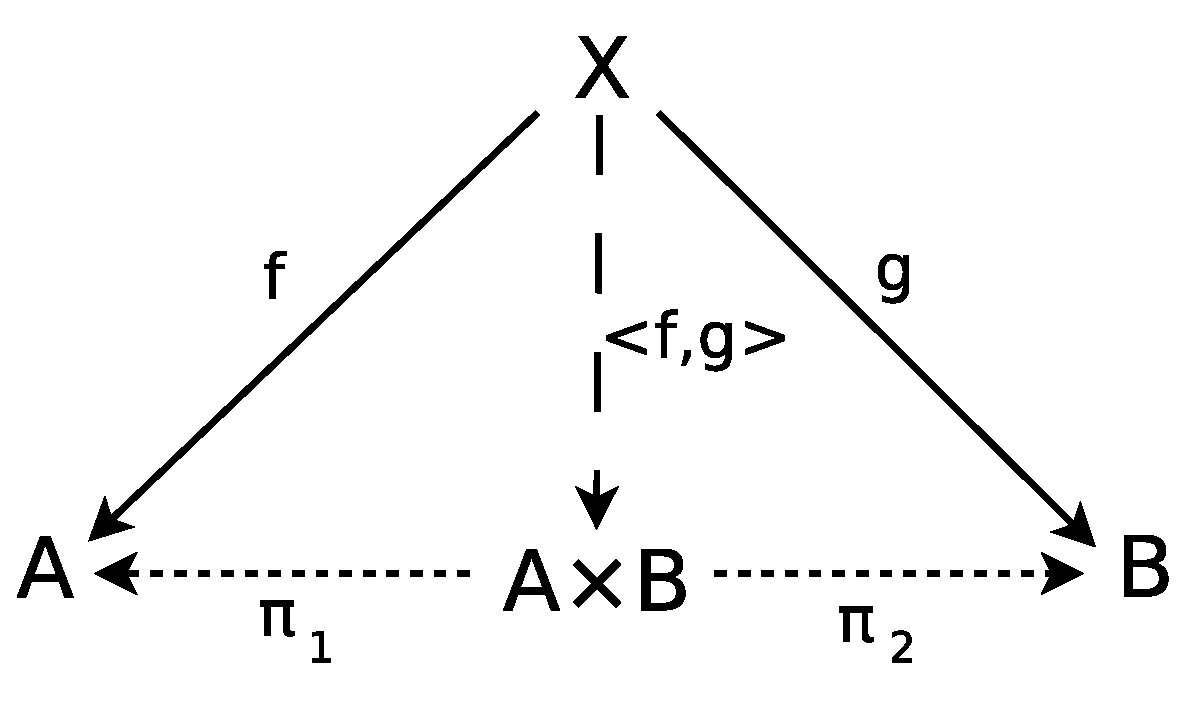
\includegraphics[scale=0.3]{images/cat_product}
    \label{magicl:fig:cat_product}
  }
  \subfloat[Coprodukt]{
    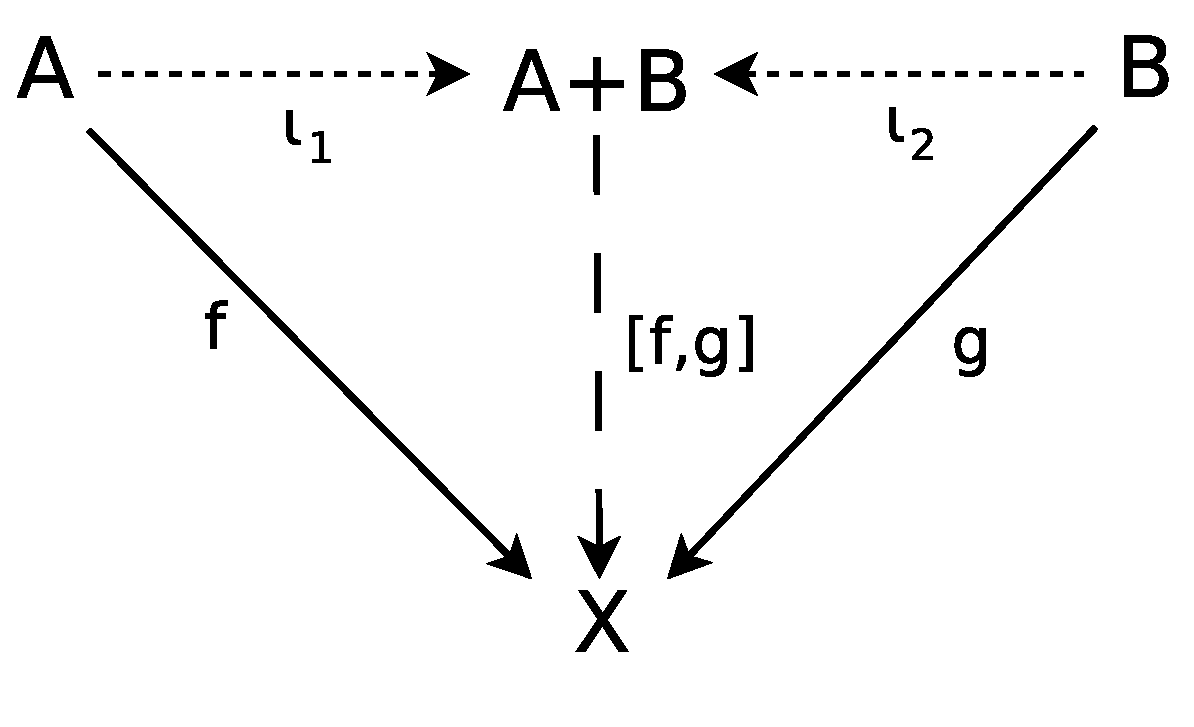
\includegraphics[scale=0.3]{images/cat_coproduct}
    \label{magicl:fig:cat_coproduct}
  }
  \caption{Kommutative Diagramme zur Definition von Produkt und Coprodukt}
\end{figure}

Man kann leicht nachvollziehen, dass das kartesische Produkt genau ein
Produkt für die Kategorie $\mathbf{Set}$ ist. $\langle f,g \rangle$ ist
hier die Funktion, die $x$ auf das Tupel $(f(x), g(x))$ abbildet.

Dreht man im Diagramm alle Pfeile um\footnote{Formal wird durch das
  ``Umdrehen'' aller Morphismen in $\mathbf{C}$ die duale Kategorie
  $\mathbf{C}^{\mathrm{op}}$ erzeugt. Entsprechend ist das Coprodukt der
  zum Produkt duale Operator.}, erhält man die Definition für das
Coprodukt:

\defi{Coprodukt}{ Ein Objekt $A + B$ mit zwei Injektionsmorphismen
  $\iota_1 : A \ato A + B$ und $\iota_2 : B \ato A + B$ ist ein
  Coprodukt von $A$ und $B$, wenn für jedes $X \in \mathrm{Ob}$ sowie
  alle $f : A \ato X$ und alle $g : B \ato X$ genau ein Morphismus
  $[f,g] : A + B \ato X$ existiert, für den \abb{cat_coproduct}
  kommutiert, d.h.  $[f,g] \circ \iota_1 = f$ und $[f,g] \circ \iota_2 =
  g$ gelten.  }

Das Coprodukt entspricht einer disjunkten Vereinigung von Mengen, also
einer Vereinigung von Mengen, die vorher explizit disjunkt gemacht
werden (sofern sie es nicht bereits sind). Dies kann beispielsweise durch
die Indizes $L$ und $R$ geschehen: $\{1,2,3\} + \{2,3,4\} =
\{1_L,2_L,3_L,2_R,3_R,4_R\}$. Der Morphismus $[f,g]$ entspricht einer
Fallunterscheidung: Auf Elemente aus $A$ wird $f$ angewendet, auf welche
aus $B$ entsprechend $g$.

\lsection[cats:func]{Funktoren}

Strukturerhaltende Abbildungen zwischen Objekten und Morphismen zweier
Kategorien werden Funktoren genannt:

\defi{Funktor}{
Ein Funktor $F=(F_{\mathrm{Ob}},F_{\mathrm{Mor}}) : \mathbf{C}
\rightarrow \mathbf{D}$ von Kategorie $C$ nach Kategorie $D$
    \begin{itemize}
    \item bildet jedes Objekt $A \in \mathrm{Ob}^{\mathbf{C}}$ auf $F_{\mathrm{Ob}}(A) \in
      \mathrm{Ob}^{\mathbf{D}}$ ab,
    \item bildet jeden Morphismus $f \in
      \mathrm{Mor}^{\mathbf{C}}_{A,B}$ auf $F_{\mathrm{Mor}}(f) \in
      \mathrm{Mor}^{\mathbf{D}}_{F_{\mathrm{Ob}}(A),F_{\mathrm{Ob}}(B)}$
      ab,
    \end{itemize}
    wobei für alle $A,B,C \in \mathrm{Ob}^{\mathbf{C}}$ und alle $f \in
    \mathrm{Mor^{\mathbf{C}}_{B,C}},g \in
    \mathrm{Mor^{\mathbf{C}}_{A,B}}$ folgende Axiome erfüllt sein
    müssen:
    \begin{itemize}
    \item Erhaltung der Komposition:
      $$F_{\mathrm{Mor}}(f \circ^{\mathbf{C}} g) =
      F_{\mathrm{Mor}}(f) \circ^{\mathbf{D}} F_{\mathrm{Mor}}(g)$$
    \item Erhaltung der Identität:
      $$F_{\mathrm{Mor}}(\mathrm{id}^{\mathbf{C}}_A) =
      \mathrm{id}^{\mathbf{D}}_{F_{\mathrm{Ob}}(A)}$$
    \end{itemize}
}

Statt $F_{\mathrm{Ob}}$ und $F_{\mathrm{Mor}}$ kann einfach $F$
geschrieben werden, wenn aus dem Kontext hervorgeht welche Abbildung
gemeint ist.

Kategorien als Objekte und Funktoren als Morphismen ergeben selbst
wieder eine Kategorie, die Kategorie der kleinen Kategorien. Kleine
Kategorien sind Kategorien, deren Klasse von Objekten eine Menge
ist. Diese Einschränkung ist nötig, da Klassen von Klassen in der
Mathematik ähnlich problematisch sind wie Mengen von Mengen.

\lsection[cats:nats]{Natürliche Transformationen}

Eine andere Möglichkeit, aus Funktoren eine Kategorien zu bilden,
besteht darin, diese als Objekte zu benutzen. Alle Funktoren $\mathbf{C}
\ato \mathbf{D}$ als Objekte bilden die sogenannte Funktorkategorie über
$\mathbf{C}$ und $\mathbf{D}$, deren Morphismen natürliche
Transformationen heißen.

\defi{Natürliche Transformation}{Eine natürliche Transformation $\alpha:F \nto
G$ ordnet jedem Objekt $A$ aus $\mathbf{C}$ einen Morphismus
$\alpha_A:F(A) \ato G(A)$ aus $\mathbf{D}$ zu, wobei für alle Objekte
$A,B$ und alle Morphismen $f:A \ato B$ aus $\mathbf{C}$ die
Gleichung
$$\alpha_B \circ F(f) = G(f) \circ \alpha_A $$
gelten muss, was dem kommutativen Diagramm in \abb{cat_nat}
entspricht.
}

Obwohl natürliche Transformationen in der Funktorkategorie Morphismen
sind, werden sie für die bessere Unterscheidung mit $\nto$ statt
$\ato$ notiert.

\fig{cat_nat}{Kommutatives Diagramm in Kategorie $\mathbf{D}$ für die Definition von
  natürlichen Transformationen}

\lsection[cats:monads]{Monaden}

Monaden setzen sich aus einem Endofunktor und zwei natürlichen
Transformationen zusammen:
\defi{Monade}{Eine Monade $(T,\eta,\mu)$ über der Kategorie $\mathbf{C}$ besteht aus
  \begin{itemize}
  \item einem Endofunktor $T:\mathbf{C} \ato \mathbf{C}$,
  \item einer natürlichen Transformation $\eta:\mathrm{id}_{\mathbf{C}} \nto T$,
  \item einer natürlichen Transformation $\mu:T^2 \nto T$,
  \end{itemize}
wobei für jedes Objekt $A$ folgende Axiome erfüllt sein müssen:
\begin{itemize}
\item Assoziativität: $$\mu_A \circ T(\mu_A) = \mu_A \circ \mu_{T(A)}$$
\item Neutrales Element: $$\mu_A \circ T(\eta_A) = \mu_A \circ \eta_{T(A)} = \mathrm{id}_{T(A)}$$
\end{itemize}
} $\mathrm{id}_\mathbf{C}:\mathbf{C} \ato \mathbf{C}$ bezeichnet hier
den Identitätsfunktor, $\mathrm{id}_{T(A)}:T(A) \ato T(A)$ dagegen den
Identitätsmorphismus. Auch diese Gleichungen lassen sich als kommutative
Diagramme darstellen. \todo{Diagramm?}

Das erste Axiom beschreibt zwei verschiedene Arten, einen Morphismus von
$T(T(T(A)))$ nach $T(A)$ zu bilden: $T(\mu_A):T(T(T(A))) \ato T(T(A))$
auf der linken Seite behält das äußere $T$ bei und verwendet $\mu$, um
das innen stehende $T(T(A))$ in $T(A)$ zu überführen. Rechts reduziert
$\mu_{T(x)}:T(T(T(A))) \ato T(T(A))$ dagegen von außen und lässt das
innere $T(A)$ unangerührt. Wird das Ergebnis dann in ein $\mu$
geschachtelt, sind innere und äußere Reduktion ununterscheidbar. Die
Gleichung lässt sich auch kurz als $\mu \circ T \mu = \mu \circ \mu T$
schreiben.

Das zweite Axiom funktioniert ähnlich, nur beschreiben diesmal beide
Seiten eine Art, den Identitätsmorphismus für das Objekt $T(A)$ zu
bilden. $T(\eta_A):T(A) \ato T(T(A)$ fügt das neue $T$ innen ein,
$\eta_{T(A)}:T(A) \ato T(T(A))$ hingegen außen.

Zu jeder Monade lässt sich eine neue Kategorie bilden, die Kleisli-Kategorie:
\defi{Kleisli-Kategorie}{
Die Kleisli-Kategorie $\mathbf{C}_K$ zur Kategorie $C$ und der
Monade $(T,\eta,\mu)$ besteht aus
\begin{itemize}
\item den Objekten von $\mathbf{C}$,
\item den Morphismen $f^{\mathbf{C}} \in
  \mathrm{Mor}^{\mathbf{C}}_{A,T(B)}$ aus $C$, die in $f \in
  \mathrm{Mor}^{\mathbf{C}_K}_{A,B}$ umbenannt werden,
\item der Identität $\mathrm{id}_A = \eta_A$,
\item der Komposition $f \circ^{\mathbf{C}_K}_{A,B,C} g = \mu_C
  \circ^{\mathbf{C}} T(f) \circ^{\mathbf{C}} g$.
\end{itemize}
}
Die Erfüllung der Kategorieaxiome wird hier nicht gezeigt, folgt aber
aus den Axiomen für Funktoren, natürliche Transformationen und Monaden.

Monaden sind in der Programmierung nützlich, da sie generisch das
Rechnen mit "`eingepackten"' Werten beschreiben. Beispielsweise könnte
$A$ für den Typ \icode{Int} und $T(A)$ für \icode{List of Int}
stehen. $\eta$ beschreibt dann die Erzeugung einer einelementigen Liste,
$\mu$ reduziert eine Liste von Listen auf eine flache Liste. Über die
Kleisli-Kategorie lassen sich damit beispielsweise nichtdeterministische
Funktionen, die eine Liste möglicher Resultate zurückliefern, elegant
Verknüpfen. Haskell \seec{haskell} benutzt Monaden unter
anderem, um Seiteneffekte in eine normalerweise pur funktionale Sprache
einzubauen, wie \sref{haskell:cats:monads} erläutert.

\lsection[cats:sum]{Zusammenfassung}

Kategorientheorie ist ein abstrakter Zweig der Mathematik, der sich mit
Morphismen (Pfeilen) zwischen Objekten (Knoten) und insbesondere der
Komposition von Morphismen befasst. Damit können unter anderem
Verarbeitungsprozesse formal und graphisch darstellbar beschrieben
werden, wobei die Möglichkeiten weit über mathematische Funktionen
hinausgehen. Über Produkte und Coprodukte können kartesische Produkte
und disjunkte Vereinigungen von Mengen auf Objekte in Kategorien
verallgemeinert werden. Mit Funktoren lassen sich Abbildungen zwischen
Kategorien beschreiben. Eine besondere Art von Funktoren sind Monaden,
welche unter anderem ``eingepackte'' Werte wie Listen beschreiben
können. Zu jeder Monade kann wiederum eine Kategorie gebildet werden,
die Kleisli-Kategorie.

Der Nutzen der Kategorientheorie für diese Arbeit besteht darin,
allgemein und abstrakt die Kombination von Verarbeitungsschritten
beschreiben zu können und somit ein formales Rahmenwerk für die
Zusammensetzung von Compilern zu liefern. Konkret zeigt sich dies in der
Umsetzung kategorientheoretischer Konzepte in Haskell.

\lchapter[haskell]{Die Sprache Haskell}

Haskell ist eine funktionale Programmiersprache, die generell sehr
mathematisch inspiriert ist. Beispielsweise sind Funktionen hier
grundsätzlich pur, d.h. ohne Nebeneffekte. Dank der Haskell-Umsetzung
von Monaden sind Berechnungen mit Nebeneffekten dennoch möglich. siehe
\sref{cats:monads} und \sref{haskell:cats:monads}. Auch
objektorientierte Konzepte gibt es hier in der Form nicht -- stattdessen
wird mittels algebraischer Datentypen und Typklassen
modelliert. Unterstützt wird dieser Ansatz durch ein statisches
Typsystem, welches praktische Features wie Typinferenz oder abhängige
Typen bereitstellt. Haskell arbeitet mit Lazy Evaluation, es werden also
Funktionen und Datenstrukturen erst dann ausgewertet, wenn diese
wirklich benötigt werden. Dies ermöglicht beispielsweise die
Konstruktion unendlicher Listen und Bäume, solange nur endliche
Teilmengen am Ende abgerufen werden.

\lsection[haskell:functions]{Funktionen}

Funktionsaufrufe in Haskell benötigen keine Klammern, sondern werden
einfach durch Leerzeichen in der Form \icode{funktion arg1 arg2 arg3}
notiert. Definitionen von Funktionen erfolgen gewöhnlich über
Gleichungen:
\begin{DIFnomarkup}\begin{code}
addTwo :: Int -> Int
addTwo x = x + 2  
\end{code}\end{DIFnomarkup}
Die erste Zeile deklariert den Typen von addTwo, welcher mit \icode{Int
  -> Int} eine Funktion ist, die einen \icode{Int} als Eingabe bekommt
und ebenfalls einen \icode{Int} zurückgibt. Typdeklarationen sind
weitestgehend optional, da die Typinferenz diese fast immer
selbstständig erschließen kann -- andererseits bieten Typdeklarationen
bereits eine gewisse Dokumentation für den Programmierer und werden
deshalb meist verwendet.

Typen von Funktionen mit mehreren Parametern erscheinen
zunächst verwirrend:
\begin{DIFnomarkup}\begin{code}
add :: Int -> Int -> Int
add x y = x + y  
\end{code}\end{DIFnomarkup}
Der Typoperator \icode{->} ist rechtsassoziierend, weshalb \icode{Int ->
  Int -> Int} äquivalent ist zu \icode{Int -> (Int -> Int)}. Streng
genommen besitzt eine Funktion in Haskell nämlich immer nur genau einen
Parameter -- eine "`Funktion mit zwei Parametern"' ist deshalb in
Wirklichkeit eine Funktion (mit einem Parameter), die eine zweite
Funktion (mit ebenfalls einem Parameter) zurückgibt. Dieses Konzept wird
als Currying bezeichnet und ermöglicht zusammen mit Funktionen höherer
Ordnung sehr elegante Formulierungen von Algorithmen. Beispielsweise
bekommt die Funktion \icode{map} mit Typsignatur \icode{(a -> b) -> [a]
  -> [b]} eine Funktion und wendet diese Elementweise auf eine Liste an
- \icode{a} und \icode{b} stehen hier für beliebige Typen. Um nun zu
jedem Element einer Liste die Zahl 5 zu addieren, kann nun der Code
\begin{DIFnomarkup}\begin{code}
map (add 5) [1, 2, 3, 4]  -- ergibt [6, 7, 8, 9]
\end{code}\end{DIFnomarkup}
verwendet werden -- \icode{add 5} erzeugt also eine Funktion, die 5 zu
ihrem Parameter addiert. Auch Funktionen können direkt auf diese Art
definiert werden:
\begin{DIFnomarkup}\begin{code}
addFiveToList :: [Int] -> [Int]
addFiveToList = map (add 5)
\end{code}\end{DIFnomarkup}

Infixoperatoren wie \icode{+} können ebenfalls vom Programmierer selbst
definiert werden -- auch die Operatorpräzedenz kann angepasst werden,
wobei Infixoperatoren grundsätzlich eine niedrigere Präzedenz als
Präfixfunktionen haben. Mittels Klammerung kann ein Infixoperator in
eine Präfixfunktion umgewandelt werden, so dass z.B. \icode{(+) 2 3}
geschrieben werden kann. Auch Infixoperatoren unterstützen direkt
Currying, so dass beispielsweise mit \icode{(-2)} eine Funktion erzeugt
wird, die vom Argument 2 subtrahiert. Für die obige, sogenannte
punktfreie\footnote{Punktfrei bedeutet, dass für Zwischenergebnisse
  keine benannten Variablen oder Parameter benötigt werden, sondern
  diese -- beispielsweise durch Currying -- implizit bleiben.} Art der
Funktionsdefinition ist auch der Kompositionsoperator \icode{.}
nützlich:
\begin{DIFnomarkup}\begin{code}
(.) :: (b -> c) -> (a -> b) -> (a -> c)
(g . f) x = g (f x)

addFiveThenMultiplyByThree :: Int -> Int
addFiveThenMultiplyByThree = (*3) . (+5)
\end{code}\end{DIFnomarkup}

Lokale Funktionen können über das Schlüsselwort \icode{where} definiert
werden:
\begin{DIFnomarkup}\begin{code}
sumSquare x y = square (x + y)
  where
    square x = x * x
\end{code}\end{DIFnomarkup}

\lsection[haskell:data]{Datentypen}

Es gibt in Haskell vier Arten von Typen: Zunächst gibt es primitive
Typen wie \icode{Char}, \icode{Int} oder \icode{Float} sowie
zusammengesetzte Typen wie Listen (Schweibweise \icode{[a, b, c]}) und Tupel (Schreibweise \icode{(a,
  b)}). Eine Sonderrolle hat hier das leere Tupel \icode{()} -- auch
"`Unit"' genannt, welches dem Typ \icode{void} in C entspricht und in
eine der beiden obigen Kategorien einzuordnen ist.

Daneben gibt es Typaliase -- beispielsweise ist der Typ String lediglich
ein Alias für Listen von Buchstaben:
\begin{DIFnomarkup}\begin{code}
type String = [Char]
\end{code}\end{DIFnomarkup}

Die letzte Kategorie sind algebraische Datentypen, welche mit dem
\icode{data}-Schlüsselwort definiert werden:
\begin{DIFnomarkup}\begin{code}
data Shape = Point
           | Circle Float
           | Rectangle Float Float
\end{code}\end{DIFnomarkup}
Hier sind \icode{Point}, \icode{Circle} und \icode{Rectangle}
verschiedene Konstruktoren, mit denen Instanzen vom Typ Shape erzeugt
werden können. Konstruktoren in Haskell können sowohl als Funktionen --
z.B. \icode{Rectangle :: Float -> Float -> Shape} -- als auch zum Pattern
Matching verwendet werden:
\begin{DIFnomarkup}\begin{code}
shapeArea :: Shape -> Float

-- Pattern Matching in Gleichungen
shapeArea Point           = 0
shapeArea (Circle r)      = pi * r * r
shapeArea (Rectangle x y) = x * y

-- Alternative mit case-Syntax
shapeArea s = case s of
                Point         -> 0
                Circle r      -> pi * r * r
                Rectangle x y -> x * y
\end{code}\end{DIFnomarkup}

Datentypen können auch durch Typvariablen parametrisiert sein,
beispielsweise beschreibt der eingebaute Typ \icode{Maybe} Werte, die
nicht immer vorhanden sind:
\begin{DIFnomarkup}\begin{code}
data Maybe a = Nothing | Just a

tryFindRecord :: Database -> ID -> Maybe Record
tryFindRecord db id = if hasRecord db id
                      then
                        Just (fetchRecord db id)
                      else
                        Nothing
\end{code}\end{DIFnomarkup}
\icode{Nothing} entspricht also in etwa \icode{null} in anderen Sprachen
-- mit dem Unterschied, dass in Haskell ganz klar definiert ist, wo dies
vorkommen kann und wo nicht.

Für den Fall, dass nur ein Konstruktor mit nur einem Argument benutzt
wird, kann statt \icode{data} auch \icode{newtype} verwendet
werden, welches vom Compiler effizienter behandelt wird, da es sich
lediglich um eine Verpackung für einen bestehenden Typen handelt. Dies
wird vor allem zusammen mit Typklassen benutzt.

\lsection[haskell:typeclasses]{Typklassen}

Oben wurden bereits Funktionen und Datentypen präsentiert, die auf
beliebige Typen anwendbar sind. Oft ist es allerdings erforderlich, die
Menge der möglichen Typen einzuschränken, beispielsweise auf Typen mit
Plus-Operator oder solche, die in Strings umgewandelt werden
können. Dies kann mit Hilfe von Typklassen erreicht werden, welche
vergleichbar mit Interfaces in objektorientierten Sprachen sowie
polymorphen Funktionen sind. Beispielsweise ist das Haskell-Äquivalent
zu Javas \icode{toString()} die Typklasse \icode{Show} gegeben:
\begin{DIFnomarkup}\begin{code}
class Show a where
  show :: a -> String
\end{code}\end{DIFnomarkup}
Algebraische Datentypen (nicht aber Typaliase) können Typklassen mittels
\icode{instance} implementieren:
\begin{DIFnomarkup}\begin{code}
instance Show Shape where
  show Point           = "point"
  show (Circle r)      = "circle with radius " ++ show r
  show (Rectangle x y) = "rectangle
\end{code}\end{DIFnomarkup}
\icode{++} ist der Haskell-Operator für Konkatenation von Listen.
Arithmetische Operationen sind ebenfalls durch Typklassen definiert, so
dass diese auch für beispielsweise komplexe Zahlen überladen werden
können.

Typvariablen können nun mittels \icode{=>} auf bestimmte Typklassen
eingeschränkt werden:
\begin{DIFnomarkup}\begin{code}
formatList :: (Show a) => [a] -> String
formatList xs = "{" ++ concat listWithSeparators ++ "}"
  where listWithSeparators :: [String]
        listWithSeparators = intersperse " - " stringList
        stringList :: [String]
        stringList = map show xs

showList [1, 2, 3] -- ergibt "{1 - 2 - 3}"
\end{code}\end{DIFnomarkup}

Derartige Typabhängigkeiten werden in dieser Arbeit in
Beispielprogrammen der Einfachheit halber oft ausgelassen - an deren
Stelle wird dann \icode{(...) =>} geschrieben.

Darüber hinaus besitzt Haskell ``Multi Type Classes'', die durch eine
Kombination von Typem implementiert werden. Auch können die Typvariablen
selbst parametrisiert sein. Letzteres ist unter anderem für einige
kategorientheoretische Begriffe nützlich, die in Haskell durch
Typklassen ausgedrückt werden.

\lsection[haskell:cats]{Kategorien in Haskell}

Die Haskell-Bibliotheken bieten viele kategorientheoretische Begriffe an,
die allerdings alle bestimmten Einschränkungen
unterliegen. Beispielsweise sind die Objekte einer Kategorie hier immer
Haskell-Typen. Die Typklasse \icode{Category} ist wie folgt definiert:
\begin{DIFnomarkup}\begin{code}
class Category cat where
  id   :: cat a a
  (.)  :: cat b c -> cat a b -> cat a c
\end{code}\end{DIFnomarkup}
Ein Typ \icode{cat}, der selbst zwei Typparameter benötigt, ist also eine
Instanz von \icode{Category}, wenn es generische Identitäts- und
Kompositionsoperatoren gibt, die für beliebige Typen $a,b,c$ benutzt
werden können. Genau genommen bestimmt \icode{Category} also keine
Kategorien, sondern vielmehr die Morphismen bestimmter Kategorien. Auch
die Axiome werden hier nicht gefordert -- vielmehr liegt es am
Programmierer, dies für eine "`vernünftige"' Programmsemantik selbst zu
verifizieren. Man sieht hier schon, dass die Haskell-Begriffe nur sehr
vage mit den mathematischen übereinstimmen -- dies wird auch bei den
weiteren Definitionen so bleiben. Die einfachste Instanz von
\icode{Category} ist \icode{(->)}, also die Kategorie der
Haskell-Funktionen, bezeichnet als $\mathbf{Hask}$.
Oft wird statt \icode{.} der \icode{>>>}-Operator (genannt "`vor"') %<<
benutzt mit \icode{f >>> g = g . f}. %<<

\lsubsection[haskell:cats:arrows]{Arrows}

Die Typklasse \icode{Arrow} beschreibt (die Morphismen von) Kategorien,
für die ein Funktor aus der Kategorie $\mathbf{Hask}$ existiert, wo man
also jeder Haskell-Funktion vom Typ \icode{a -> b} einen Morphismus vom
Typ \icode{cat a b} zuordnen kann. Dies ist deshalb sinnvoll, da viele
(Haskell-)Kategorien "`mehr"' können als normale Funktionen, formal eine zu
$\mathbf{Hask}$ isomorphe Unterkategorie besitzen. Beispielsweise
benutzt MagicL "`Funktionen, die fehlschlagen können"' oder "`Funktionen
mit Nebeneffekten"' als Kategorien, die jeweils auch normale Funktionen
enthalten. Zusätzlich wird eine Operation auf Tupeln gefordert, aus der
sich ein Produkt zusammensetzen lässt -- ein Coprodukt wird zunächst nicht gefordert:
\begin{DIFnomarkup}\begin{code}
class (Category ar) => Arrow ar where
  arr   :: (a -> b) -> ar a b
  first :: ar a b  -> ar (a, c) (b, c)
\end{code}\end{DIFnomarkup}
\icode{arr} ist der Funktor, der jede Funktion auf einen Arrow
abbildet\footnote{Die Typen werden hierbei auf sich selbst abgebildet.}.
\icode{first} ist eine Funktion, die aus einem Arrow einen Arrow auf
Tupeln macht, der nur auf dem ersten Element arbeitet, das zweite
dagegen unverändert durchschleift. Somit lassen sich zusätzliche Werte
weiterreichen, außerdem lassen sich aus \icode{first} sinnvolle
Operationen ableiten:

\begin{DIFnomarkup}\begin{code}
  second :: ar a b -> ar (c, a) (c, b)
  second = arr swap >>> first f >>> arr swap
    where swap (x, y) = (y, x)

  (***) :: ar a b -> ar a' b' -> ar (a, a') (b, b')
  f *** g = first f >>> second g

  (&&&) :: ar a b -> ar a b' -> ar a (b, b')
  f &&& g = arr diag >>> (f *** g)
    where diag x = (x,x)
\end{code}\end{DIFnomarkup} % <<

\begin{itemize}
\item \icode{second} ist analog zu \icode{first}, reicht allerdings das erste
Element unverändert weiter.
\item \icode{f *** g} wendet \icode{f} auf das
erste Element, danach \icode{g} auf das zweite Element eines Tupels
an.
\item \icode{f &&& g} ist nun die Haskell-Entsprechung von $\langle f,g
\rangle$ in \dref{Produkt}. \icode{f} und \icode{g} werden also beide
auf die Eingabe angewendet und deren Ergebnisse zu einem Tupel
zusammengesetzt.
\end{itemize}

Möchte man einen Arrow mit einer Funktion verknüpfen, gibt es mit
\begin{DIFnomarkup}\begin{code}
f >>^ func = f >>> arr func
\end{code}\end{DIFnomarkup}% <<
noch etwas syntaktischen Zucker.

\lsubsection[haskell:cats:coproducts]{Coprodukte: Die Klasse \texttt{ArrowChoice}}

Die Haskell-Entsprechung zu einer disjunkten Vereinigung ist der
\icode{Either}-Datentyp, der folgendermaßen definiert ist:
\begin{DIFnomarkup}\begin{code}
data Either a b = Left a | Right b
\end{code}\end{DIFnomarkup}
Coprodukte für Arrows werden durch die Klasse \icode{ArrowChoice} beschrieben:
\begin{DIFnomarkup}\begin{code}
class (Arrow ar) => ArrowChoice ar where
  left :: ar a b -> ar (Either a c) (Either b c)
\end{code}\end{DIFnomarkup}
Auch hier wird mit \icode{left} nur eine einfache Operation gefordert,
aus der sich anschließend alles weitere konstruieren lässt. Diese
Funktion wandelt einen Arrow von \icode{a} nach \icode{b} um in
einen Arrow von \icode{Either a c} nach \icode{Either b c}. Bei einem
\icode{Left}-Wert wird also der ursprüngliche Arrow angewendet, ein
\icode{Right}-Wert wird dagegen unverändert weitergereicht.
\begin{DIFnomarkup}\begin{code}
  right :: ar a b -> ar (Either c a) (Either c b)
  right f = arr swap >>> left f >>> arr swap
    where swap (Left x)  = Right x
          swap (Right x) = Left x

  (+++) :: ar a b -> ar a' b' -> ar (Either a a') (Either b b')
  f +++ g = left f >>> right g

  (|||) :: ar a c -> ar b c -> ar (Either a b) c
  f ||| g = (f +++ g) >>> arr dropEither
    where dropEither (Left x)  = x
          dropEither (Right x) = x

\end{code}\end{DIFnomarkup} %<<
Die Definitionen sind weitgehend analog zu den entsprechenden
Produkt-Operationen:
\begin{itemize}
\item \icode{right} bearbeitet nur \icode{Right}-Werte, während
  \icode{Left}-Werte unverändert bleiben.
\item \icode{f +++ g} wendet auf \icode{Left}-Werte \icode{f} an, auf
  die anderen \icode{g}.
\item Haben \icode{f} und \icode{g} denselben Rückgabetyp, kann
  \icode{f ||| g} verwendet werden, welches das in diesem Fall unnötige
  \icode{Either} verschwinden lässt. Dies entspricht $[f,g]$ in
  \dref{Coprodukt}
\end{itemize}

\lsubsection[haskell:cats:functors]{Funktoren}

Die Haskell-Bibliotheken definieren eine Klasse \icode{Functor}, welche
allerdings nur Endofunktoren über der Kategorie $\mathbf{Hask}$ repräsentieren:
\begin{DIFnomarkup}\begin{code}
class Functor f where
  fmap :: (a -> b) -> f a -> f b
\end{code}\end{DIFnomarkup}
Ein Datenkonstruktor \icode{f} ist also Instanz von \icode{Functor},
wenn die Operation \icode{fmap} Funktionen von \icode{a} nach \icode{b}
auf Funktionen von \icode{f a} nach \icode{f b} abbildet. Der
mathematische Funktor besteht hier also aus \icode{(f,fmap)}.

Diese Arbeit benutzt stattdessen eine eigene \icode{Functor}-Klasse,
die verschiedene Kategorien zulässt:
\begin{DIFnomarkup}\begin{code}
class Functor f ar | f -> ar where
  lift :: ar a b -> f a b
\end{code}\end{DIFnomarkup}
Die Arrows \icode{f} und \icode{ar} bilden eine Instanz von
\icode{Functor}, wenn eine \icode{lift}-Operation \icode{ar}-Arrows auf
\icode{f}-Arrows zwischen den gleichen Typen abbildet -- wobei der Typ
\icode{f} den Typ \icode{ar} bestimmt. Der mathematische Funktor
hier ist also \icode{(id,lift)}. Im Vergleich zu Haskells
Standard-\icode{Functor} ist diese Version also in den Kategorien
allgemeiner, aber dafür spezieller in der Abbildung der Objekte, da hier
die Identität vorgeschrieben ist. Man könnte auch dies allgemein
formulieren -- aber im Rahmen von MagicL reicht die spezielle Version
bisher aus.

Alle hier verwendeten \icode{Functor}-Instanzen konstruieren aus einem
\icode{Arrow}-Typ einen zweiten mit zusätzlichen Eigenschaften,
z.B. erweitert der \icode{FailFunctor} einen Arrow-Typ um mögliches
Scheitern. Die Instanz-Deklaration dafür sieht im Gerüst folgendermaßen
aus (die Details werden in \sref{arrowparser:fail} erläutert):
\begin{DIFnomarkup}\begin{code}
newtype FailFunctor ar a b = ...

instance (Arrow ar) => Functor (FailFunctor ar) ar where
  lift f = ...
\end{code}\end{DIFnomarkup}

\lsubsection[haskell:cats:monads]{Monaden}

Die Typklasse \icode{Monad} aus den Haskell-Bibliotheken beschreibt
Monaden über der Kategorie $\mathbf{Hask}$. $\eta$ aus
\sref{cats:monads} heißt hier \icode{return}, statt $\mu$ wird der
Operator \icode{>>=} %<<
mit anderer Signator gefordert:
\begin{DIFnomarkup}\begin{code}
class Monad m where
  return :: a -> m a
  (>>=)  :: m a -> (a -> m b) -> m b
\end{code}\end{DIFnomarkup} % <<
Es gibt auch eine genaue Entsprechung von $\mu$, die hier \icode{join}
heißt:
\begin{DIFnomarkup}\begin{code}
join :: (Monad m) => m (m a) -> m a
join x = x >>= id
\end{code}\end{DIFnomarkup} % <<

Zu jeder Haskell-Monade \icode{m} lässt sich wieder die
Kleisli-Kategorie bilden, die die Datentypen als Objekte sowie die
Funktionen \icode{a -> m b} als Morphismen enthält. Die
Haskell-Bibliotheken stellen hierfür den Datentyp \icode{Kleisli}
bereit:
\begin{DIFnomarkup}\begin{code}
newtype Kleisli m a b = Kleisli (a -> m b)

instance (Monad m) => Category (Kleisli m)
  where id = Kleisli return
        Kleisli f . Kleisli g = Kleisli composed
          where composed x = g x >>= f

instance (Monad m) => Arrow (Kleisli m)
  where arr fun = Kleisli (return . fun)
        first (Kleisli f) = Kleisli tupleF
          where tupleF (x, z) = f x >>= (\ y -> return (y, z))
\end{code}\end{DIFnomarkup} %<<

Arrows und Monaden werden beide verwendet, um abstrakt Verknüpfungen von
speziellen Operationen zu beschreiben. Arrows sind allgemeiner, denn
jede Monade lässt sich beispielsweise mittels \icode{Kleisli} auf einen
entsprechenden Arrow abbilden. Auf der anderen Seite entspricht aber
nicht jedem Arrow eine Monade, denn aus den Arrow-Operationen allein
lässt sich \icode{>>=} % <<
nicht konstruieren. Hierfür wird zusätzlich die Operation \icode{app}
benötigt, die von der Typklasse \icode{ArrowApply} definiert wird (für
Details siehe \cite[S. 18f]{Hughes}):
\begin{DIFnomarkup}\begin{code}
class (Arrow ar) => ArrowApply ar where
  app :: ar (ar a b, a) b
\end{code}\end{DIFnomarkup}
Mit \icode{app} wird also ein Arrow bereitgestellt, der als Parameter
einen weiteren Arrow sowie eine Eingabe bekommt, um dann den übergebenen
Arrow auf die Eingabe anzuwenden. Damit ist es möglich, Arrows
einzusetzen, die erst im Verarbeitungsprozess und in Abhängigkeit der
Eingabedaten erzeugt werden -- eine Eigenschaft, die Monaden generell
besitzen. Dies wird beispielsweise in \sref{arrowparser} wichtig für
die Konstruktion von kontextsensitiven Parsern.

Instanzen der Klasse \icode{ArrowChoice} sind vollständig äquivalent zu
Monaden.  Dies wirft die Frage auf, weshalb Haskell überhaupt Monaden
benutzt und nicht alles über Arrows realisiert. Zum einen gibt es dafür
historische Gründe: Monaden waren bereits 1993 in Haskell präsent
\cite[S.23ff]{HaskellHistory}, während Arrows erst 1998 von John Hughes
vorgeschlagen wurden, da sich spezielle Parser mit statischen
Komponenten nicht durch Monaden ausdrücken lassen \cite{Hughes}. Zum
anderen bieten Monaden aber auch Vorzüge: Die Definition einer Monade
ist etwas kürzer, da keine \icode{first}-Funktion für Produkte
bereitgestellt werden muss -- wie obiger Code zeigt lässt sich dies
bereits mittels \icode{>>=} % <<
ausdrücken. Zudem gibt es für Monaden in Haskell die praktische
\icode{do}-Notation:
\begin{DIFnomarkup}\begin{code}
do x <- foo
   y <- bar x
   return (x, y)
\end{code}\end{DIFnomarkup}
ist syntaktischer Zucker für
\begin{DIFnomarkup}\begin{code}
foo >>= (\ x ->
  bar x >>= (\ y ->
    return y))
\end{code}\end{DIFnomarkup} % <<
und ermöglicht eine Schreibweise, die imperativen Programmen ähnelt --
dies ist kein Zufall, denn Nebeneffekte werden in Haskell ebenfalls mit
einer Monade beschrieben (siehe \sref{haskell:cats:monads:examples:io}),
so dass auch dort die \icode{do}-Notation benutzt werden kann. Diese
Verwendung erklärt auch nachträglich den Namen \icode{return}, wobei es
sich noch immer um die $\eta$-Transformation handelt und nicht etwa ein
syntaktisches \icode{return}-Statement wie in imperativen Sprachen
üblich.

Für Arrows gibt es mit \icode{proc} auch eine Notation, mit der
Zwischenergebnisse benannt werden können. Diese ist aber weniger simpel
und elegant als das Monadenäquivalent. Auf der anderen Seite eignen sich
Arrows besser als Monaden für eine punktfreie Schreibweise, d.h. einer
Schreibweise ohne Zwischenvariablen, bei der ausschließlich auf
Komposition zurückgegriffen wird. Punktfreie Notation wird auch bei
Definitionen von Funktionen oft verwendet und ist für viele
Haskell-Programmierer natürlicher und eleganter.

\lsubsubsection[haskell:cats:monads:examples]{Beispiele für Monaden}

\lparagraph[haskell:cats:monads:examples:maybe]{\icode{Maybe}}

Funktionen, die fehlschlagen können, lassen sich in der Form \icode{a
  -> Maybe b} darstellen. Möchte man mehrerer solcher Funktionen
verketten, werden normalerweise viele Fallunterscheidungen benötigt, da
bei jeder Funktion die Rückgabe geprüft und nur im Erfolgsfall die
nächste aufgerufen muss. Haskell vereinfacht dies, indem \icode{Maybe}
zur Monade erklärt wird:
\begin{DIFnomarkup}\begin{code}
instance Monad Maybe
  where return = Just
        (Nothing >>= _) = Nothing
        (Just x  >>= f) = f x
\end{code}\end{DIFnomarkup} % <<
Obiges Code-Beispiel, mit einer Typanschrift auf die Maybe-Monade
festgelegt 
\begin{DIFnomarkup}\begin{code}
(do x <- foo
    y <- bar x
    return (x, y)) :: Maybe (Integer, Integer)
\end{code}\end{DIFnomarkup}
wird wie folgt interpretiert: Wenn \icode{foo} erfolgreich ist, wird das
Ergebnis (lokal) in \icode{x} gespeichert. Ist daraufhin \icode{bar x}
ebenfalls erfolgreich, wird dieses in \icode{y} gespeichert und
schließlich der Wert \icode{Just (x, y)} zurückgegeben. Schlägt eine der
Funktionen fehl, ist das Ergebnis \icode{Nothing}.

\lparagraph[haskell:cats:monads:examples:io]{\icode{IO}}

Jede Programmiersprache benötigt für die reale Welt Möglichkeiten,
Operationen mit Nebeneffekten wie das Schreiben von Dateien oder solche,
die von externen Nebeneffekten abhängen, wie das Lesen von Dateien,
auszuführen. Dies lässt sich zunächst schwer in eine puren Sprache wie
Haskell integrieren. Die \icode{IO}-Monade bietet hier eine Lösung: Man
stelle sich einen fiktiven Datentyp \icode{World} vor, der den gesamten
Zustand der externen Welt enthält. \icode{IO a} ist nun eine Funktion,
die die Welt liest und eine andere Welt sowie ein a zurückgibt:
\begin{DIFnomarkup}\begin{code}
newtype IO a = World -> (World, a)
\end{code}\end{DIFnomarkup}
Zum Verketten zweier \icode{IO}-Operationen wird die von der ersten
zurückgegebene Welt an die zweite übergeben. Damit dies nicht von Hand
geschehen muss, wird \icode{IO} wieder als Monade deklariert. Nun gibt
es aber natürlich keinen wirklichen \icode{World}-Typen -- in
Wirklichkeit wird also der Haskell-Compiler alles, was mit \icode{IO}
verpackt ist, in imperativen Code übersetzen. Dennoch gelingt dadurch
die saubere Trennung von puren Code und solchem, der Nebeneffekte
enthalten kann. Da ist nicht möglich ist, eine "`Auspack-Funktion"'
\icode{IO a -> a} zu definieren\footnote{Es gibt eine solche Funktion in
  Haskell, die aber normalerweise nicht verwendet werden sollte.}, das
Gegenteil aber mit \icode{return} möglich ist, kann imperativer Code
immer funktionalen, funktionaler Code aber niemals imperativen
enthalten. Die äußerste Funktion jedes Haskell-Programms, \icode{main},
wird deshalb immer in der \icode{IO}-Monade ausgeführt.

Dank der Kleisli-Kategorie lassen sich mittels \icode{IO} auch Arrows
bereitstellen, die Nebeneffekte enthalten:
\begin{DIFnomarkup}\begin{code}
type IOArrow = Kleisli IO
\end{code}\end{DIFnomarkup}

\lsection[haskell:sum]{Zusammenfassung}

Haskell ist eine pur funktionale, statisch typisierte Programmiersprache
mit Typinferenz. Konzepte wie Currying und Funktionen höherer Ordnung
ermöglichen einen eleganten, modularen und punktfreien
Programmierstil. Für die Definition eigener Datenstrukturen stehen
algebraische Datentypen bereit, die in etwa die Rolle einer Klasse in
objektorientierten Sprachen einnehmen. Es können auch Typvariablen
verwendet werden, die deutlich mächtiger und präziser sind als
beispielsweise Java-Generics \cite{JavaGenerics}. Die Rolle von
Interfaces nehmen in Haskell Typklassen ein.

In Haskell werden mit Arrows und Monaden auch einige
kategorientheoretische Konzepte umgesetzt und in Form von Typklassen
bereitgestellt. Während Arrows allgemeiner und konzeptionell einfacher
sind und optimal für eine punktfreie Formulierung von Algorithmen sind,
können Monaden teilweise einfacher implementiert werden und ermöglichen
mittels do-Notation eine punktierte Schreibweise mit benannten
Zwischenvariablen. Alle Monaden lassen sich über die Kleisli-Kategorie
in Arrows umwandeln und viele Arrows in Monaden.

Haskell selbst nutzt Monaden, um Funktionen mit Seiteneffekten sauber in
die ansonsten pure Sprache integrieren zu können. Die Monade \icode{IO}
lässt sich als verstecktes Weiterreichen eines \icode{World}-Zustandes von
Funktion zu Funktion veranschaulichen.

MagicL legt den Schwerpunkt auf Arrows und beschreibt so allgemein
Compiler. Parser werden hier als Spezialform eines Compilers gesehen.

\todo{anonyme Fns}

\lchapter[arch]{Grundlegende Architektur}

\todo{Parser, Makros etc. als Arrows}
\todo{Komponenten, Schichtenmodell}

\lchapter[arrowparser]{Arrow-basierte Parser}

Parser sind für die Umwandlung von Zeichenketten in Objekte
verantwortlich und werden deshalb für Code-Generatoren benötigt, die
ihre Eingaben aus Text-Dateien beziehen. In vielen Programmiersprachen
ist die direkte Implementation von Parsern relativ aufwändig, weshalb
der entsprechende Code häufig selbst aus einer DSL wie JavaCC
generiert wird, die eine EBNF-ähnliche Notation mit bestimmten
Abschnitten kombiniert, die Code in der Zielsprache enthalten.

\todo{Parser in MagicL erklären (kleine Bausteine, gesamter Parser)}

Die Haskell-Bibliothek Parsec \cite{Parsec} hingegen beschreitet einen
anderen Weg: Hier werden Parser als monadische Funktionen konstruiert,
so dass diese direkt in Haskell und ohne spezielle Syntax beschrieben
werden können. Parser-Kombinatoren wie \icode{<|>} oder \icode{many}
entsprechen den EBNF-Operationen. Darüber hinaus können sogar eigene
Kombinatoren definiert werden -- beispielsweise könnte \icode{sepBy}
Listen mit Trennzeichen einlesen, wenn ein Parser für die Elemente und
einer für die Trennzeichen übergeben werden. Aus diesem Grund können
komplexe Parser in Parsec oft deutlich eleganter konstruiert werden als
mit anderen Parser-Generatoren -- außerdem können hier auch
kontextsensitive Sprachen wie XML ausnahmslos verarbeitet werden (siehe
\cite[S. 3]{Parsec}), was mit anderen Bibliotheken nicht möglich ist.

Es wäre möglich gewesen, Parser in MagicL mittels Parsec zu
konstruieren. Dennoch wurde für diese Arbeit entschieden, ein eigenes,
allgemeineres Framework für die Parser-Konstruktion zu
entwickeln. Dadurch wird neben der freien Auswahl des
Token-Typs\footnote{Auch Parsec lässt es allerdings zu, dass statt
  Zeichenketten auch Listen beliebiger Token eingelesen werden können.}
auch eine freie Auswahl der Kategorie ermöglicht, in der Parser
ausgeführt werden. Beispielsweise kann \icode{IOArrow} benutzt werden,
um Debug-Ausgaben oder andere Nebeneffekte in Parser einzubauen. Dies
ist in Parsec nicht möglich.

MagicL benutzt Arrows und Funktoren, um möglichst allgemein zu
sein. Alles, was im Rahmen dieser Arbeit implementiert wurde, hätte zwar
auch wie in Parsec über Monaden und Monaden-Transformatoren konstruiert
werden können. Dennoch besteht die Möglichkeit, dass später Ergänzungen
vorgenommen werden sollen, die sich nicht mittels Monaden ausdrücken
lassen -- beispielsweise ein effizienterer Parsing-Algorithmus, der
sowohl statische als auch dynamische Komponenten enthält, wie ihn
Swierstra und Duponcheel entworfen haben (siehe
\cite[S. 8ff]{Hughes}). Zudem sind Arrows als programmiersprachliche
Umsetzung von Morphismen anschaulicher als Monaden und besitzen eine
praktische graphische Repräsentation.

Wenn allerdings kontextsensitive Parser wie in Parsec konstruiert werden
sollen, müssen die zugrundeliegenden Arrows äquivalent zu Monaden sein,
also die Typklasse \icode{ArrowApply} implementieren.

Dieses Kapitel entwickelt nun schrittweise einen Parser-Datentyp durch
die Kombination einfacher Funktoren. Parser zeichnen sich hauptsächlich
durch zwei Eigenschaften aus:
\begin{itemize}
\item Sie können fehlschlagen sowie Alternativmöglichkeiten im Falle des
  Scheiterns besitzen.
\item Sie bearbeiten einen Zustand, der die Position im Eingabe-Stream
  beschreibt.
\end{itemize}
Diese beiden Eigenschaften werden von den Datentypen \icode{FailFunctor}
und \icode{StateFunctor} umgesetzt.

\lsection[arrowparser:fail]{Fehlschlagende Arrows}

Berechnungen von $A$ nach $B$, die fehlschlagen können, sollen zwei
mögliche Resultate haben. Im Erfolgsfall wird ein normaler Rückgabewert
aus $B$ geliefert, während im Falle eines Scheiterns eine Fehlermeldung
als String zurückgegeben wird -- im Gegensatz zur \icode{Maybe}-Monade,
die im Fehlerfall nur ein \icode{Nothing} liefert. Der Rückgabetyp ist
deshalb das Coprodukt $\mathrm{String}+B$. Statt Morphismen von $A$ nach
$B$ werden nun Morphismen von $A$ nach $\mathrm{String}+B$ benutzt. Um
den aufrufenden Code nicht komplizierter zu machen, empfiehlt es sich,
diese Änderung in einer neuen Kategorie $\mathbf{C}_f$ zu
verstecken. $f_{f} : A \rightarrow B$ aus der neuen Kategorie wird
abgebildet auf $f : A \rightarrow \mathrm{String} + B$. Der Arrow
$\mathrm{fail}_{f} : \mathrm{String} \rightarrow a$ in $C_{f}$ schlägt
immer fehl und entspricht $fail : \mathrm{String} \rightarrow
\mathrm{String} + a$ in $C$.

Der Operator $\bigvee : Mor_{A,B} \times Mor_{A,B}
\rightarrow Mor_{A,B} $ bietet Alternativen, wodurch ein Backtracking im
Fehlerfall möglich wird. Um Morphismen aus
$\mathbf{C}$ in $\mathbf{C}_f$ benutzen zu können, gibt es den Funktor
$\mathrm{lift}_f:\mathbf{C} \ato \mathbf{C}_f$, welcher die
unveränderte, d.h. gelingende Operation für die neue Kategorie
übernimmt.

Die Haskell-Entsprechung von $\mathrm{String}+B$ ist \icode{Either
  String b}, was sich mit \icode{Failable b} abkürzen lässt, wenn man
den parametrisierten Typ \icode{Failable} einführt:

\begin{DIFnomarkup}\begin{code}
type Failable a = Either String a
\end{code}\end{DIFnomarkup}

Der Fehlerfall wird durch \icode{Left String} ausgedrückt, ein Erfolg
durch \icode{Right a}. Fehlschlagende Arrows nun sind in MagicL durch den
Typ \icode{FailFunctor} implementiert:

\begin{DIFnomarkup}\begin{code}
newtype FailFunctor ar a b = FailF (ar a (Failable b))

instance (Arrow ar) => Functor (FailFunctor ar) ar where
    lift f = FailF (f >>> arr Right)
\end{code}\end{DIFnomarkup} % <<

Arrows von \icode{a} nach \icode{b}, die fehlschlagen können, sind also
Arrows von \icode{a} nach \icode{Failable b}, die in den zusätzlichen
Konstruktor \icode{FailF} eingebettet wurden. Um einen normalen Arrow
\icode{f} aus \icode{ar} nach \icode{FailFunctor ar} zu "`liften"', wird
der Rückgabewert in ein \icode{Right} gebettet und der resultierende
Arrow in \icode{FailF}.
Der Arrow \icode{fail} wird in eine \icode{Arrow} erweiternde Typklasse
ausgegliedert, so dass dieser auch in anderen Kategorien bereitgestellt
werden könnte:

\begin{DIFnomarkup}\begin{code}
class (Arrow ar) => ArrowFail ar where
  fail :: ar String a

instance (ArrowChoice ar) => ArrowFail (FailFunctor ar) where
  fail = FailF (arr Left)
\end{code}\end{DIFnomarkup}

Dem Oder-Operator $\bigvee$ entspricht in Haskell \icode{<+>}, welcher
von der Typklasse \icode{ArrowPlus} aus den Haskell-Bibliotheken
bereitgestellt wird und für \icode{FailFunctor} wie folgt implementiert
ist:

\begin{DIFnomarkup}\begin{code}
instance (ArrowChoice ar) => ArrowPlus (FailFunctor ar) where
  FailF f <+> FailF g = FailF ((f &&& id) >>> arr proc >>> (g ||| arr Right))
   where proc :: (Either a b, c) -> Either c b
         proc (Left  _, y) = Left y
         proc (Right x, _) = Right x
\end{code}\end{DIFnomarkup} % <<

Es werden also zunächst \icode{f} und die Identität parallel evaluiert --
dies ist nötig, um die Eingabe "`durchzuschleifen"'. Anschließend
erfolgt ein Verarbeitungsschritt um das Tupel aufzulösen: Scheitert
\icode{f}, wird dessen Ausgabe weggeschmissen, im Erfolgsfall die
Eingabe. Anschließend wird im Fehlerfall \icode{g} auf die Eingabe
angewendet, bei Erfolg wird das Ergebnis wieder in ein \icode{Right} eingepackt.

\fig{cat_fail}{Komposition beim Fail-Funktor}

Die Typabhängigkeit von \icode{ArrowChoice} ist nötig, weil
\icode{FailFunctor ar} nur dann ein \icode{Arrow} ist, wenn \icode{ar}
ein Coprodukt anbietet. Denn die Komposition in $C_{f}$ ist definiert
durch $g_{f} \circ f_{f} = ([fail,g] \circ f)_{f}$, was in Haskell
\begin{DIFnomarkup}\begin{code}
FailF g . FailF f = FailF (f >>> (arr Left ||| g))
\end{code}\end{DIFnomarkup} %<<
entspricht. Tritt in \icode{f} ein Fehler auf, wird dieser also wieder
in ein \icode{Left} eingepackt und zurückgegeben. Ansonsten wird das
durch \icode{|||} implizit aus dem \icode{Right}-Konstruktor ausgepackte
Ergebnis an \icode{g} weitergereicht.

\abb{cat_fail} zeigt die Komposition in $\mathbf{C}_f$ und deren
Zurückführung auf ein Coprodukt in $\mathbf{C}$. Die Funktion, die $f_f$
auf $f$ abbildet, kann nicht Teil eines Funktors sein. Ein solcher
müsste nämlich das Objekt $B$ sowohl auf $\mathrm{String}+B$ (bei der
Transformation von $f$ als auch auf $B$ selbst (bei $g$) abbilden.

\todo{Beispiel Fehlermeldung}

\lsection[arrowparser:state]{Arrows mit Zuständen}

Zustände lassen sich ähnlich zu einem Arrow hinzufügen. Über Produkte
wird der Zustandstyp $S$ (z.B. eine Stream-Position oder der
\textit{Seed} eines Zufallszahlengenerators) an Domäne und Codomäne
heran gehängt, was wieder in einer neuen Kategorie $C_{s}$ versteckt
wird. Ein Morphismus $f_{s} : A \rightarrow B$ der neuen Kategorie
wird entsprechend abgebildet auf $f = A \times S \rightarrow B \times
S$. Da hier im Gegensatz zum Fail-Funktor Domäne und Codomäne gleich
abgebildet werden, ist diese Abbildung Teil eines Funktors $F_s: C_{s}
\ato C$. \abb{cat_state} zeigt die Komposition in $\mathbf{C}_s$ und die
Rückführung auf die ursprüngliche Kategorie.

\fig{cat_state}{Komposition in $\mathbf{C}_s$ und Rückführung auf
  $\mathbf{C}$ durch $F_s$}

In MagicL gibt es die Typklasse \icode{StateFunctor}, die einen weiteren
Typparameter \icode{s} für den Zustand bekommt:

\begin{DIFnomarkup}\begin{code}
newtype StateFunctor s ar a b = StateF (ar (a, s) (b, s))

instance (Arrow ar) => Functor (StateFunctor s ar) ar where
    lift = StateF . first
\end{code}\end{DIFnomarkup} % <<

Die "`geliftete"' Version eines Arrows soll den Zustandsparameter
unverändert weitergeben -- dies entspricht genau der
\icode{first}-Funktion aus \sref{haskell:cats:arrows}.

Das Lesen und Schreiben von Zuständen wird von den Funktionen \icode{get} und
\icode{put} bereitgestellt, welche in der Typklasse \icode{ArrowState}
definiert werden:

\begin{DIFnomarkup}\begin{code}
class (Arrow ar) => ArrowState s ar | ar -> s where
  get :: ar a s
  put :: ar s ()

instance (Arrow ar) => ArrowState s (StateFunctor s ar)
  where
    get = StateF (arr (\ (_, state) -> (state, state)))
    put = StateF (arr (\ (state, _) -> ((), state)))
\end{code}\end{DIFnomarkup}

\icode{get} ignoriert also den Eingabewert und gibt den aktuellen
Zustand zurück, während \icode{put} den übergebenen Zustand
"`abspeichert"' und (bis auf diesen) nichts zurückgibt.

\todo{Verwendungsbeispiel}

\lsection[arrowparser:parse]{Der Parse-Funktor}

Nun lassen sich obige Kategorie-Erweiterungen zu einer Parser-Kategorie
$\mathbf{C}_p = \mathbf{C}_{fs}$ zusammensetzen, d.h. die ursprüngliche
Kategorie wird zunächst um Fehler zu $\mathbf{C}_f$, danach um Zustände
zu $\mathbf{C}_p$ erweitert. Die Reihenfolge hier ist wichtig, damit ein
Morphismus $A \ato B$ aus $\mathbf{C}_p$ auf $A \times S \ato
\mathrm{String} + B \times S$ in $\mathbf{C}$ abgebildet wird und nicht
auf $A \times S \ato (\mathrm{String} + B) \times S$, wie es andersherum
wäre. Denn das Coprodukt muss "`außen"' stehen, um im Kontrollfluss
zuerst bearbeitet zu werden und somit ein Backtracking im Fehlerfall zu
ermöglichen.

Backtracking wird allerdings zu einem Problem, wenn man sinnvolle
Fehlermeldungen produzieren will. Man stelle sich einen Parser für die
(als regulärer Ausdruck beschriebene\footnote{Hierbei sollen eckige und
  geschweifte Klammern keine besondere Bedeutung besitzen, der Punkt für
  ein beliebiges Zeichen und der Stern für beliebige Wiederholungen
  stehen.}) Grammatik \texttt{\{.*\}|[.*]} vor, die eine beliebige
Zeichenkette in geschweiften oder eckigen Klammern beschreibt. Beim
Eingabewort \texttt{\{ABC} scheitert zunächst aufgrund der fehlenden
schließenden Klammer die erste Alternative, woraufhin die zweite
probiert wird. Das Wort beginnt aber nicht mit \texttt{[}, so dass der
  Parser beispielsweise mit der Meldung \texttt{"'Expected [, got \{"'}
    scheitert. Diese Meldung beschreibt den Fehler schlecht --
    stattdessen möchte man nach dem Lesen von \texttt{\{} das
    Backtracking deaktivieren, denn bereits hier ist klar, dass die
    andere Alternative nicht mehr in Betracht kommt. Dies führt zu einer
    sinnvolleren Fehlermeldung wie \texttt{"'Expected \}, got end of
      stream"'}.

Ein derartiger "`nicht-auffangbarer"' Fehler lässt sich durch das
Einbauen einer weiteren Möglichkeit des Scheiterns ermöglichen, wir
definieren also $\mathbf{C}_p = \mathbf{C}_{ffs}$ und bieten eine
Funktion \icode{forceParser} an, die einen (Sub-)Parser derart
modifiziert, dass, falls dieser scheitert, der Fehler in die "`innere"'
und damit nicht-recover-fähige Fail-Kategorie übernommen wird. Hiervon
wird beispielsweise bei der Funktion \icode{macro}
\sees{arrowparser:sexpparser} Gebrauch gemacht.

Der \icode{ParseFunctor} ist in MagicL wie folgt definiert::
\begin{DIFnomarkup}\begin{code}
newtype ParseFunctor t ar a b =
  P (StateFunctor
     [t]
     (FailFunctor (FailFunctor ar))
     a
     b)
\end{code}\end{DIFnomarkup}
Als Zustandstyp wird ein Stream (als Liste repräsentiert) vom Token-Typ
\icode{t} benutzt.  Dank der Implementation als Funktor ist die
Kategorie, in der der Parser ausgeführt wird, frei wählbar. So können
rein funktionale Parser in $Hask_p$ konstruiert werden. Benötigt man
aber Debug Outputs (z.B. bei der Suche einer Endlosschleife) oder andere
Seiteneffekte, kann $\mathbf{IO}_p$ benutzt werden. In MagicL werden
diese Kategorien durch die Typaliase \icode{FunParser} sowie
\icode{IOParser} bereitgestellt:
\begin{DIFnomarkup}\begin{code}
type FunParser t a b = ParseFunctor t (->) a b
type IOParser  t a b = ParseFunctor t IOArrow a b
\end{code}\end{DIFnomarkup}
Eine geeignete innere Kategorie könnte
sogar interaktive Debugger, Netzwerktransparenz oder sonstige Features
anbieten. Auch der variable Token-Typ erzeugt viele Möglichkeiten:
Textdateien können mit \icode{Char}, Bit-Streams mit \icode{Bool} oder
\sexp{}-Streams mit \icode{Sexp} verarbeitet werden.

\todo{Mehr Top-Down-Argumente}

\lsection[arrowparser:lib]{Parser-Library}

MagicL beinhaltet eine Parser-Bibliothek, in der u.a. viele simple
Parser-Konstruktoren definiert sind. Hier ein paar
Beipiele\footnote{Abhängigkeiten der Typparameter werden hier der
  Übersichtlichkeit halber weggelassen.}:
\begin{itemize}
\item \icode{empty :: ParseFunctor t ar a a}\\
  gibt seinen Eingabewert unverändert zurück, wenn der Stream leer ist.
\item \icode{takeWhen :: (t -> Bool) -> (t -> String) -> ParseFunctor t ar a
    t}\\
  testet den ersten Token mit einem Prädikat. Im Erfolgsfall (\icode{True}) wird der
  Token zurückgegeben, ansonsten wird der Token an eine Funktion
  übergeben, die daraus eine Fehlermeldung aufbaut.
\item \icode{member :: [t] -> ParseFunctor t ar a t}\\
  testet, ob der erste Token in der übergebenen Liste vorkommt.
\item \icode{streamEq ::  [t] -> ParseFunctor t ar a [t]}\\
  prüft, ob die ersten $n$ Token mit den Elementen der übergebenen Liste
  übereinstimmen, und gibt diese im Erfolgsfall zurück. Für \icode{t =
    Char} wird hier also ein String gelesen.
\end{itemize}

Alle diese Funktionen (und deren Negationen) geben Parser mit nützlichen
Fehlermeldungen zurück.

Weiterhin gibt es viele Arrow-Kombinatoren, mit denen Parser,
vergleichbar mit den Operationen der Erweiterten Backus-Naur-Form (EBNF)
\cite[S.43ff]{EBNF}, verschaltet werden können. Mit den bisher eingeführten
Operatoren sind bereits Konkatenation (\icode{>>>}) %<<
und Alternative (\icode{<+>}) abgedeckt, darüber hinaus gibt es für
Instanzen von \icode{ArrowPlus} unter anderem folgende Funktionen:

\begin{DIFnomarkup}\begin{code}
optional :: (...) => ar a b -> ar a (Maybe b)
optional f = (f >>^ Just) <+> constArrow Nothing
  where constArrow x = arr (\ _ -> x)

many :: (...) => ar a b -> ar a [b]
many f = many1 f <+> constArrow []

many1 :: (...) => ar a b -> ar a [b]
many1 f = consArrow f (many f)
  where consArrow :: ar a b -> ar a [b] -> ar a [b]
        consArrow f g = (f &&& g) >>^ (\ (x,xs) -> x : xs)

skip :: (...) => ar a b -> ar a a
skip f = (f &&& id) >>^ snd

sepBy :: (...) => ar a c -> ar a b -> ar a [b]
sepBy sep item =
  optional (consArrow item (many (skip sep >>> item))) >>^ unMaybeList
    where
      unMaybeList  Nothing  = []
      unMaybeList (Just xs) = xs
\end{code}\end{DIFnomarkup} % <<

\icode{optional} erzeugt einen Arrow, der, sollte der übergebene Arrow
scheitern, \icode{Nothing} zurückgibt -- dabei aber "`erfolgreich"'
bleibt. Dies entspricht \icode{[ ]} in EBNF. Hierbei erzeugt
\icode{constArrow Nothing} einen Arrow, der die Eingabe ignoriert und
konstant \icode{Nothing} zurückgibt. Eine (optionale) Wiederholung (in EBNF
\icode{\{ \}}) erzeugt \icode{many}, \icode{many1} verlangt mindestens
ein Vorkommen. Die Hilfsfunktion \icode{consArrow} nimmt zwei
Arrows an und erzeugt daraus einen, der das Element, welches der erste
zurückgibt, vor die Liste hängt, die der zweite zurückliefert.
\icode{skip} ignoriert das Resultat eines Arrows und gibt
stattdessen seine Eingabe zurück -- Zustandsänderungen kann der
ignorierte Arrow aber dennoch bewirken. \icode{sepBy} ist ein
komplizierteres Beispiel und ermöglicht das Parsen von Listen mit
Trennzeichen. Dafür bekommt die Funktion zwei Arrows übergeben:
\icode{sep} soll ein Trennzeichen, \icode{item} ein Element lesen. Es
wird zunächst ein \icode{item}, dann beliebig viele, von (ignorierten)
\icode{sep} angeführte \icode{item}-Elemente gelesen. Das ganze ist noch
in ein \icode{optional} gebettet, damit auch eine leere Liste gelesen
werden kann. Die Rückgabe wird mittels \icode{unMaybeList} vom durch
\icode{optional} erzeugten \icode{Maybe}-Datentyp befreit, so dass statt
\icode{Nothing} eine leere Liste zurückgegeben wird, wenn nichts gelesen
werden kann.

\lsection[arrowparser:sexp]{Beispiel: Ein Parser für \sexps{}}

\sexps{} sind in MagicL wie folgt definiert:
\begin{DIFnomarkup}\begin{code}
data Sexp = Symbol String
          | Node [Sexp]
\end{code}\end{DIFnomarkup}

Aufgrund der Einfachheit dieser Struktur und der praktischen
Parser-Library ist es möglich, in vier kurzen Zeilen einen Parser zu
entwerfen, der als Text repräsentierte \sexps{} in die typisierte
Repräsentation überführt:

\begin{DIFnomarkup}\begin{code}
whitespace = skip (many (member " \t\n"))
\end{code}\end{DIFnomarkup}
Zunächst wird Whitespace als beliebige Anhäufung von Spaces, Tabs und
Newlines definiert, die ignoriert werden soll.
\begin{DIFnomarkup}\begin{code}
parseSymbol = many1 (notMember " \t\n()") >>^ Symbol
\end{code}\end{DIFnomarkup} % <<
Ein Symbol ist eine Kette von Zeichen, die weder Whitespace noch
Klammern sind. Dieses wird gleich an den \icode{Symbol}-Konstruktor
übergeben, um den Typ \icode{Sexp} zu erhalten.
\begin{DIFnomarkup}\begin{code}
parseNode = skip (eq '(') >>> (many parseSexp >>^ Node) >>> skip (eq ')')
\end{code}\end{DIFnomarkup} % <<
Ein Knoten ist eine von Klammern umgebene Liste von \sexps{}, die
mittels \icode{Node}-Konstruktor zu einem \sexp{} wird.
\begin{DIFnomarkup}\begin{code}
parseSexp = whitespace >>> (parseSymbol <+> parseNode) >>> whitespace
\end{code}\end{DIFnomarkup} % <<
Ein \sexp{} ist nun entweder ein Symbol oder ein Knoten, wobei davor und
danach Whitespace auftreten darf.

\begin{figure}[h]
\begin{DIFnomarkup}\begin{code}
whitespace  = skip (many (member " \t\n"))
parseSymbol = many1 (notMember " \t\n()") >>^ Symbol
parseNode   = skip (eq '(') >>> (many parseSexp >>^ Node) >>> skip (eq ')')
parseSexp   = whitespace >>> (parseSymbol <+> parseNode) >>> whitespace    
  \end{code}\end{DIFnomarkup}
  \caption{Ein kompletter \sexp{}-Parser in vier Zeilen}
  \label{magicl:fig:sexp_parser}
\end{figure}

\abb{sexp_parser} zeigt noch einmal den gesamten Parser. Ein
Beispielaufruf könnte wie folgt aussehen:
\begin{code}
runParser parseSexp "(this is (an s-expr))"  ==> Node [Symbol "this", ...]
\end{code}
Tritt bei Lesen ein Fehler auf, wird automatisch eine brauchbare
Fehlermeldung ausgegeben, z.B.
\begin{DIFnomarkup}\begin{code}
runParser parseSexp "(test) )"  ==>  Empty stream expected: ")"
\end{code}\end{DIFnomarkup}

\lsection[arrowparser:sexpparser]{Parser auf \sexps}

Der Begriff \sexp{}-Parser bezeichnet in dieser Arbeit Parser, die
Listen von \sexps{} als Eingabe und einen beliebigen Typ als Ausgabe
haben. Der Parser aus dem vorigen Abschnitt ist daher in dieser
Terminologie ein Char-Parser, der \sexps{} zurückliefert. Entsprechend
ist der Typ \icode{SexpParser} in MagicL definiert als \icode{IOParser} (für
Seiteneffekten wie Debug-Ausgaben) vom Token-Typ \icode{Sexp} ohne
explizite Eingabe und mit beliebigem Rückgabewert:
\begin{DIFnomarkup}\begin{code}
type SexpParser a = IOParser Sexp () a  
\end{code}\end{DIFnomarkup}
Die Parser-Bibliothek an sich kann bereits Streams von \sexps{}
verarbeiten. Es gibt allerdings bisher keine komfortablen Operationen,
um das Innere einer \sexp{} zu testen oder zu verarbeiten. Da ein
\sexp{} selbst wieder eine Liste und damit ein Stream ist, bietet es
sich an, diesen ebenfalls über einen "`inneren Parser"' zu verarbeiten.

Beispielsweise könnte eine Liste von Personen folgenderweise
repräsentiert sein\footnote{Dieses Format ist unnötig redundant und
  sollte vermutlich besser durch \icode{(persons Franz Walter Heinz)}
  ersetzt werden -- aber es handelt sich ja lediglich um ein Beispiel.}:
\begin{DIFnomarkup}\begin{code}
(person Franz)
(person Walter)
(person Heinz)
\end{code}\end{DIFnomarkup}

Ein Parser, der aus dieser Eingabe eine Liste von Namensstrings
produzieren soll, würde mit der bisherigen Bibliothek so aussehen:

\begin{DIFnomarkup}\begin{code}
parsePerson :: SexpParser String
parsePerson = take >>^ proc >>> (fail ||| id)
  where proc (Node [Symbol "person", Symbol x]) = Right x
        proc y = Left ("Not a person: " ++ show y)
parsePersons :: SexpParser [String]
parsePersons = many parsePerson
\end{code}\end{DIFnomarkup} % <<
Hierbei liest der Befehl \icode{take} den nächsten Token bedingungslos
ein.

Die Verarbeitung von Hand mittels \icode{Node} und \icode{Symbol} im
Pattern-Matching ist relativ umständlich. Deswegen gibt es eine Reihe
nützlicher Hilfsfunktionen für die Konstruktion von \sexp{}-Parsern:

\begin{itemize}
\item \icode{takeSexp} liest eine \sexp{} vom Stream und wandelt diese
  für die Unterscheidung zwischen Symbolen und Knoten mittels
  \icode{|||} in das Coprodukt \icode{Either String [Sexp]} um.
\item \icode{takeSymbol} erwartet ein Symbol und gibt dieses als String
  zurück -- ansonsten wird eine Fehlermeldung ausgegeben.
\item \icode{symbolMacro name = skip (eq (Symbol name))} akzeptiert nur
  das Symbol mit Namen \icode{name}.
\item \icode{takeNode} erwartet einen Knoten und gibt diesen als Liste
  von \sexps{} zurück.
\item \icode{compNode innerComp} verarbeitet einen Knoten, indem der
  übergebene Parser \icode{innerComp} auf das Knoteninnere angewendet
  wird. Da Parser in MagicL immer als Compiler definiert werden (siehe
  \sref{magicl:compinterface}), heißt diese Funktion nicht
  \icode{parseNode}
\item \icode{macro name innerComp} % <<
  konstruiert nun einen Parser, der wie ein Makro das erste Element des
  Knotens mit dem Symbol \icode{name} vergleicht und im Erfolgsfall die
  restlichen Elemente mit \icode{innerComp} verarbeitet. Danach wird
  sichergestellt, dass der Knoten auch wirklich vollständig gelesen
  wurde -- will man dies nicht, da man den Rest ignoriert, gibt es die
  Funktion \icode{looseMacro} mit identischer Signatur.
\end{itemize}
Das obige Beispiel lässt sich nun umschreiben:
\begin{DIFnomarkup}\begin{code}
parsePerson  = macro "person" takeSymbol
parsePersons = many parsePerson
\end{code}\end{DIFnomarkup}

\icode{macro} benutzt \icode{forceParser} aus
\sref{arrowparser:parse}, um das Backtracking auszuhebeln, sobald das
Symbol übereinstimmt, was wieder für bessere Fehlermeldungen
sorgt. Allerdings bedeutet dies, dass Code wie
\begin{DIFnomarkup}\begin{code}
macro "foo" (symbolMacro "bar") <+> macro "foo" (symbolMacro "baz")
\end{code}\end{DIFnomarkup}
nicht erwartungsgemäß funktioniert:
\begin{DIFnomarkup}\begin{code}
(foo bar)   => ()  d.h. Erfolg, kein Ergebnis
(foo baz)   => Symbol bar expected: baz
\end{code}\end{DIFnomarkup}
Es sollte deshalb immer nur ein Makro für jeden Begriff benutzt und
eine etwaige Oder-Verknüpfung ins Innere verlegt werden -- hier also:
\begin{DIFnomarkup}\begin{code}
macro "foo" (symbolMacro "bar" <+> symbolMacro "baz")
\end{code}\end{DIFnomarkup}

\lsection[arrowparser:sum]{Zusammenfassung}

Parser werden in MagicL durch die Verschachtelung zweier Funktoren
implementiert, die bestehende Arrows um bestimmte Möglichkeiten
erweitern. Der \icode{FailFunctor} realisiert die Möglichkeit, mit einer
Fehlermeldung zu Scheitern und per Backtracking Alternativen zu
probieren. Der \icode{StateFunctor} setzt das Durchreichen von Zuständen
um und wird benutzt, um den noch zu lesenden Stream als Liste zu
verwalten. Der \icode{ParseFunctor} kombiniert beides, wobei der
\icode{FailFunctor} doppelt verwendet wird, um auch Fehler zu
ermöglichen, die nicht durch Backtracking zu beheben sind. Dies ist
hilfreich, um teilweise sinnvollere Fehlermeldungen zu erhalten.

Eine Parser-Bibliothek stellt neben Konstruktoren wie \icode{member}
auch Kombinatoren wie \icode{many} bereit, die eine EBNF-artige
Formulierung ermöglichen. Die Parser sind sehr allgemein, da sowohl
Rückgabetyp als auch Token-Typ variabel sind, so dass mehr als nur
Strings eingelesen werden können. Makros werden in MagicL als Parser auf
\sexps{} definiert, die auch Subausdrücke rekursiv mit Parsern
verarbeiten können.

\todo{Diskussion: Welche Anforderungen erfüllt, wie nah an kontextfreien
Grammatiken?}

\lchapter[magicl]{Weitere Komponenten von MagicL}

Die im letzen Kapitel vorgestellten Arrow-basierten Parser und Makros
sowie die damit in \cref{sexphs} und \cref{sexpcomp} implementierten
Sprachen sind das Herzstück von MagicL. Darüber hinaus gibt es
allerdings noch weitere Komponenten, die in den folgenden Abschnitten
vorgestellt werden.

\todo{auf Anforderungen beziehen}

\lsection[magicl:code]{Repräsentation von Quelltext}

Die meisten Frameworks für \cgen{} erzeugen Quelltext aus
String-basierten Templates und daher mit
Low-Level-Methoden. Syntaktische Konstrukte werden daher oft wiederholt,
was zu häufigen Syntaxfehlern und einem relativ hohen Wartungsaufwand
führt. Es würde beispielsweise viel Arbeit bedeuten, alle in einer
generierten Java-Klasse definierten Arrays in Collections umzuwandeln,
wenn die \icode{\{A, B, C\}}-Syntax überall direkt benutzt
wurde. Hilfreich wäre es, wenn stattdessen überall ein Sub-Template
\icode{genList} aufgerufen würde -- nun müsste nur noch eine Stelle
verändert werden um die erwünschte Anpassung durchzuführen. Diese
Abstraktion ist auch mit einigen String-basierten Templates
realisierbar. Ein weiteres Problem aber ist die Formatierung -- denn auch
generierter Quelltext wird eventuell gelesen werden. Ein Template für
\icode{for}-Schleifen kann den Schleifenkörper nicht korrekt einrücken,
da der Einrückungslevel immer relativ zur -- leider im Template
unbekannten -- äußeren Einrückung ist.  Wenn vorhanden, kann der erzeugte
Code daher an einen Formatierer wie Jalopy \cite{Jalopy} übergeben werden --
für ein sprachunabhängiges Framework ist diese Option aber nicht
zufriedenstellend.

MagicL verfolgt einen anderen Ansatz und definiert ein typisiertes
Modell für formatierten Code samt Compiler nach String. Hier handelt es
sich um einen Nachbau des von Philip Wadler in
\cite[S.223ff]{FunOfProgramming} vorgestellten Pretty-Printers. Die
elementaren Konstruktor-Funktionen sind:
\begin{DIFnomarkup}\begin{code}
newline :: Code
text    :: String -> Code
append  :: Code   -> Code -> Code
group   :: Code   -> Code
indent  :: Int    -> Code -> Code
\end{code}\end{DIFnomarkup}

\icode{newline}, \icode{text} und \icode{append} sollten selbsterklärend
sein. \icode{group} versucht den übergebenen \icode{Code} auf eine Zeile
zu bekommen, indem es alle Zeilenumbrüche durch Leerzeichen
ersetzt. Wird dabei allerdings die geforderte Zeilenlänge (im
Standard-Compiler 70) überschritten, wird die ursprüngliche Version mit
Zeilenumbrüchen genommen. \icode{indent} rückt den übergebenen
\icode{Code} bei jedem Zeilenumbruch um $n$ Zeichen ein, z.B. würde
\begin{DIFnomarkup}\begin{code}
indent 2 (conc [text "hallo", newline, text "welt"])
\end{code}\end{DIFnomarkup}
den Text
\begin{DIFnomarkup}\begin{code}
hallo
  welt
\end{code}\end{DIFnomarkup}
ergeben -- dabei verbindet \icode{conc :: [Code] -> Code} eine Liste
mittels \icode{append}. Darüber hinaus gibt es viele weitere allgemeine
Funktionen wie
\begin{DIFnomarkup}\begin{code}
  joinBy :: Code -> [Code]
\end{code}\end{DIFnomarkup}
-- welche einen Separator benutzt, um eine Liste zusammenzufügen.
\begin{DIFnomarkup}\begin{code}
joinBy "; " [text "foo", text "bar", text "baz"]
\end{code}\end{DIFnomarkup}
würde also
\begin{DIFnomarkup}\begin{code}
foo; bar; baz
\end{code}\end{DIFnomarkup}
ergeben. Aus diesen allgemeinen Funktionen werden dann Abkürzungen für
syntaktische Programmiersprachenelemente abgeleitet, wie
\icode{commaSep} für eine Komma-separierte Liste oder \icode{parens},
\icode{braces} und \icode{brackets} für die drei gängigen Arten der
Klammerung.

\lsubsection[magicl:code:prettysexp]{Beispiel: Ein Pretty-Printer für \sexps{}}

\sexps{} sollen wie folgt formatiert werden: Passt der gesamte Ausdruck
noch auf die aktuelle Zeile, werden normal Leerzeichen verwendet:
\begin{DIFnomarkup}\begin{code}
(a b (c d) e)
\end{code}\end{DIFnomarkup}
Wird die gewünschte Breite aber überschritten, soll jeder Subausdruck
auf einer eigenen Zeile stehen, wobei alle bis auf den ersten um zwei
Zeichen eingerückt werden:
\begin{DIFnomarkup}\begin{code}
(a
  b
  (c d)
  e)
\end{code}\end{DIFnomarkup}
Dies lässt sich mit dieser rekursiven Funktion erreichen:
\begin{DIFnomarkup}\begin{code}
layoutSexp :: Sexp -> Code
layoutSexp (Symbol sym)    = text sym
layoutSexp (Node children) = format (map layoutSexp children)
  where format = parens . group . indent2 . lines
\end{code}\end{DIFnomarkup} %<<
Alternativ könnte \icode{layoutSexp} auch als \sexp{}-Parser
spezifiziert werden.

\lsection[magicl:compinterface]{Generische Compiler-Schnittstelle}

Um das Parser-Framework herum soll ein wieder möglichst allgemeines
Interface für die Beschreibung von Compilern entstehen, so dass
beispielsweise Parser und gewöhnliche Verarbeitungsfunktionen
komfortabel kombiniert werden können. Ziel ist die selbstständige Suche
nach einem passenden Compiler, wenn nur Ein- und Ausgabetyp spezifiziert
sind. Compiler sollen unter anderem als pure Funktionen oder als Parser
spezifiziert werden können.

Ein Compiler von \icode{a} nach \icode{b} ist in MagicL etwas, was sich
in eine Operation mit \icode{a} als Ein- und \icode{b} als Ausgabe
überführen lässt. Diese Operation kann im allgemeinen Nebeneffekte
enthalten, weshalb IOArrow verwendet wird. Typen, mit denen sich
Compiler repräsentieren lassen, implementieren die Typklasse
\icode{Executable}:
\begin{DIFnomarkup}\begin{code}
class Executable x a b | x -> a b where
  toIO :: x -> IOArrow a b
\end{code}\end{DIFnomarkup}
\icode{x} ist selbst ein parametrisierter Typ, der die Ein- und
Ausgabetypen \icode{a} und \icode{b} bereits determiniert. Die einfachsten
Instanzen von \icode{Executable} werden durch IOArrows selbst sowie pure
Funktionen gebildet:
\begin{DIFnomarkup}\begin{code}
instance Executable (IOArrow a b) a b where
  toIO = id

instance Executable (a -> b) a b where
  toIO f = Kleisli (return . f)
\end{code}\end{DIFnomarkup}
Auch Parser sind ausführbar, sofern der zugrundeliegende Arrow-Typ es
ist:
\begin{DIFnomarkup}\begin{code}
instance (...) => Executable (ParseFunctor t ar () a) [t] a where
  toIO = toIO . execParser
\end{code}\end{DIFnomarkup}
Ein Parser von \icode{()} nach \icode{a} mit Token-Typ \icode{t} wird
demnach beim Ausführen zu einem \icode{IOArrow} von \icode{[t]} nach
\icode{a}. Der bei der Parser-Komposition noch implizite
Stream-Parameter wird hier also explizit gemacht -- der vom Parser
implizit zurückgegebene Stream wird verworfen. Sollte es erforderlich
sein, einen Parser mit weiteren Parametern aufzurufen oder auch den
Rest-Stream zu erhalten, muss statt \icode{Executable} direkt mit dem
Parser-Modul gearbeitet werden.

Nun soll es möglich sein, einen ausführbaren Typen zu benutzen, um einen
eindeutigen Compiler von \icode{a} nach {b} einzurichten. Dies geschieht
über die Typklasse \icode{Compilable}:
\begin{DIFnomarkup}\begin{code}
class (Executable x a b) => Compilable x a b | a b -> x where
  comp :: x
\end{code}\end{DIFnomarkup}
Da es nur einen ausgezeichneten Compiler von \icode{a} nach \icode{b}
geben kann, determinieren \icode{a} und \icode{b} gemeinsam \icode{x},
wobei die umgekehrte Abhängigkeit ebenfalls -- von \icode{Executable}
geerbt -- besteht. Es handelt sich also um eine 1:1-Beziehung. Die
Spezifikation eines simplen funktionalen Compilers würde so aussehen:
\begin{DIFnomarkup}\begin{code}
instance Compilable (A -> B) A B where
  comp x = ...
\end{code}\end{DIFnomarkup}
Der Parser, der einen \sexp{} aus einem String erzeugt, kann auch als
Compiler spezifiziert werden:
\begin{DIFnomarkup}\begin{code}
instance Compilable (FunParser Char () Sexp) String Sexp where
  comp = many parseSexp
\end{code}\end{DIFnomarkup}
Auf diese Weise kann der Parser automatisch durch einen Aufruf von
\icode{comp} gefunden werden.

Da Listen- und Maybe-Datentypen von Parsern fast immer mit \icode{many}
und \icode{optional} verarbeitet werden, können für \icode{[a]} und
\icode{Maybe a} Standard-Parser bereitgestellt werden, die den
bestehenden Parser für \icode{a} mit diesen Funktionen transformieren:
\begin{DIFnomarkup}\begin{code}
instance (Compilable (ParseFunctor t ar () a) [t] a, ...) =>
  Compilable (ParseFunctor t ar () [a]) [t] [a] where
    comp = many comp

instance (Compilable (ParseFunctor t ar () a) [t] a. ...) =>
  Compilable (ParseFunctor t ar () (Maybe a)) [t] (Maybe a) where
    comp = optional comp
\end{code}\end{DIFnomarkup}
Nun können beispielsweise auch Streams von \sexps{} durch den Aufruf von
\icode{comp :: FunParser Char () [Sexp]} geparst werden, ohne dass dieser
  Parser manuell spezifiziert wurde.

Zuletzt "`vergisst"' die Typklasse \icode{Compiler} den zur Definition
verwendeten Typen und bietet eine allgemeine Umwandlung von A nach B an:
\begin{DIFnomarkup}\begin{code}
class Compiler a b where
  compile :: IOArrow a b

instance (Compilable x a b) => Compiler a b where
  compile = toIO comp
\end{code}\end{DIFnomarkup}
Nun kann ein beliebiger Compiler ungeachtet seines Implementationstyps
einfach über einen explizit typisierten \icode{compile}-Aufruf, wie etwa
\\\icode{compile :: IOArrow String [Sexp]}, gefunden werden. Leider ist
es aufgrund des Haskell-Typsystems nicht möglich, dass sogar
Kombinationen aus Compilern selbstständig gefunden werden. Hierfür
müsste das Typsystem eine Prolog-artige Tiefensuche unterstützen, was
zumindest derzeit noch nicht der Fall ist. 

Um die Kompilation von Textdateien zu vereinfachen, wird die Funktion
\icode{compileStr} definiert, welche ein \icode{Executable} von
\icode{a} nach \icode{b} in eine imperative Haskell-Funktion von
\icode{String} nach \icode{String} umwandelt. Dies funktioniert
allerdings nur, wenn bereits Standardcompiler von \icode{String} nach
\icode{a} und von \icode{b} nach \icode{String} bekannt sind.
\begin{DIFnomarkup}\begin{code}
compileStr :: (Compiler String a, Executable x a b, Compiler b String) =>
               x -> String -> IO String
compileStr f = runKleisli $ compile >>> toIO f >>> compile
\end{code}\end{DIFnomarkup} % $
Für die Erzeugung selbstständiger Compiler benutzt \icode{compiler}
stdin als Eingabe- und stdout als Ausgabe-Stream:
\begin{DIFnomarkup}\begin{code}
compiler :: (Compiler String a, Executable x a b, Compiler b String) => x -> IO ()
compiler f = do
  input <- getContents
  output <- compileStr f input
  putStr output  
\end{code}\end{DIFnomarkup}
Damit kann ein Compiler als Stand-Alone-Programm erzeugt und mit Hilfe
von Ein- und Ausgabeumleitungen auf Dateien angewendet werden:
\begin{DIFnomarkup}\begin{code}
module MyFileCompiler where
-- einige Import-Anweisungen

main = compiler myCompiler

==== Erzeugung des Programms ====

ghc MyFileCompiler.hs  -- einige Parameter ausgelassen
=> MyFileCompiler

==== Aufruf ====

./MyFileCompiler <inFile >outFile
\end{code}\end{DIFnomarkup}

\lsection[magicl:test]{Test-Framework}

MagicL enthält ein primitives Unit-Test-Framework für die Überprüfung
einzelner Compiler (und damit auch Parser und Makros). Zunächst werden
dafür die Eingaben und erwarteten Ausgaben als Strings in Listen
notiert:
\begin{DIFnomarkup}\begin{code}
exprCases = [ ( "(Str 42)"                    -- Sexp-Haskell 
                , "\"42\"" )                  -- Haskell 

              , ( "(Str a  b c)"              -- Sexp-Haskell 
                , "\"a b c\"" )               -- Haskell 

              , ( "(List a b (Str c))"        -- Sexp-Haskell 
                , "[a, b, \"c\"]" )           -- Haskell 

              , ( "(foo a (bar b c) d)"       -- Sexp-Haskell 
                , "(foo a (bar b c) d)" )     -- Haskell 

              , ( "(map + myList)"            -- Sexp-Haskell 
                , "(map (+) myList)" )        -- Haskell 
              ]  
\end{code}\end{DIFnomarkup}
Dieses Beispiel spezifiziert, wie einige Ausdrücke der im nächsten
Kapitel vorgestellten Sprache \sexp{}-Haskell nach Haskell übersetzt
werden sollen. Durchgeführt wird ein Testlauf mit der Funktion
\icode{testCompiler}:
\begin{DIFnomarkup}\begin{code} 
testCompiler :: 
  (Compiler String a, Executable x a b, Compiler b String) => 
  String -> x -> [(String, String)] -> IO ()
\end{code}\end{DIFnomarkup}
Als Eingaben werden ein Namensstring, der Compiler selbst (als
Executable-Instanz, damit nicht nur fest verdrahtete Compiler getestet
werden können) sowie eine Liste von Testfällen erwartet. Das Testen
von Makros ist ein Spezialfall, da hier meist kein direkter
Standard-Compiler vom Rückgabetyp nach \icode{String} bereitsteht --
stattdessen wird gewöhnlich ein Compiler nach \icode{Code}
angeboten. Die Funktion \icode{testMacro} schaltet deshalb den
Standard-Compiler nach \icode{Code} hinter ein
Makro:
\begin{DIFnomarkup}\begin{code}
testMacro name mac testCases = 
  (testCompiler name 
                ((toIO mac >>> compile) :: IOArrow [Sexp] Code)
                testCases)
\end{code}\end{DIFnomarkup}
Der Aufruf für obige Testfälle sieht beispielsweise wie folgt aus:
\begin{DIFnomarkup}\begin{code}
testMacro "expr" (comp :: SexpParser Expr) exprCases  
\end{code}\end{DIFnomarkup}
Das zu testende Makro wird hier durch einen typisierten Aufruf von
\icode{comp} referenziert. Alternativ können auch benannte Makros
verwendet werden.

\lsection[magicl:sum]{Zusammenfassung}

Für die Repräsentation von Quelltext benutzt MagicL das typisierte
Modell \icode{Code}. Dadurch ist es möglich, mit Einrückung, Klammerung
etc. auf strukturelle Weise umzugehen, was die Anfälligkeit für
Syntaxfehler gegenüber String-basierten Templates verringert. Dieses
Modell kann anschließend in Quelltext übersetzt werden.

Für die allgemeine Spezifikation von Verarbeitungsprozessen stellt
MagicL eine Schnittstelle mit drei Typklassen bereit, mit der einzelne
Compiler mit beliebigen Arrows oder auch komplett anderen Methoden
konstruiert und kombiniert werden können. Alles, was in einen
\icode{IOArrow} von \icode{a} nach \icode{b} überführt werden kann,
implementiert die Typklasse \icode{Executable}. Instanzen dieser Klasse
können dann verwendet werden, um mit \icode{Compilable} feste Compiler
zwischen zwei Typen zu verdrahten, die dann mittels Typinferenz
automatisch gefunden werden können. Für die leichtere Benutzung können
diese dann über die Polymorphe Funktion \icode{compile} aus der
Typklasse \icode{Compiler} angesprochen werden, die den intern
verwendeten \icode{Executable}-Typ versteckt.

Ein minimales Test-Framework ermöglicht Unit Testing einzelner Compiler
oder Makros.

\lchapter[sexphs]{\sexp{}-Haskell}

Die Implementation einiger Komponenten von MagicL erfordert selbst
\cgen{} -- beispielsweise muss eine etwaige DSL für Template-basierte
\sexp{}-Erzeugung nach Haskell kompiliert werden. Da diese Generierung
ebenfalls auf \sexp{}-Basis erfolgen soll, wird in diesem Abschnitt
eine minimale, funktionale \sexp{}-Sprache vorgestellt, die in legalen
Haskell-Quellcode kompiliert wird.

Bei dem Entwurf eines neuen Compilers muss zunächst entschieden
werden, ob die Verarbeitung mittels typisierter Modell oder direkt
untypisiert auf den \sexps{} erfolgen soll. Typisierte Modelle erhöhen
den Entwicklungsaufwand\footnote{Die zukünftige Entwicklung einer
  geeigneten DSL zur Modellbeschreibung, aus der sowohl das typisierte
  Modell als auch Compiler generiert werden, könnte den
  Entwicklungsaufwand wieder reduzieren.}, führen aber zu früherer
Fehlererkennung in Compilern und ermöglichen eine automatische
Compiler-Auswahl. Der Haskell-Generator beschreitet diesen Weg und
dient damit gleichzeitig als Anschauungsbeispiel für die Benutzung
typisierter Modelle. Rein \sexp{}-gestützte Kompilation hingegen wird
in \cref{sexpcomp} behandelt.

\lsection[sexphs:spec]{Spezifikation}

\sexp{}-Haskell soll im Wesentlichen eine in \sexp{} gegossene Version
von Haskell sein -- mit nur wenigen Anpassungen, wo diese sinnvoll
erscheinen. Eine vollständige Abdeckung aller Haskell-Konzepte muss im
Prototyp nicht gegeben sein, da diese bei Bedarf nachgepflegt werden
können. Zudem sind einige Konzepte wie \icode{let} und \icode{where}
redundant, so dass nur eines von beiden benötigt wird. 

\lsubsection[sexphs:spec:funs]{Funktionen}
Funktions- oder Konstruktoraufrufe müssen in der \sexp{}-Version immer
geklammert werden, können aber unverändert nach Haskell übernommen
werden:
\begin{DIFnomarkup}\begin{code}
(myFun 1 4 52)              Sexp-Haskell
=>
(myFun 1 4 52)              Haskell
\end{code}\end{DIFnomarkup}
Haskell-Infixoperatoren werden in Präfixnotation überführt und können
in dieser beliebig viele Argumente annehmen wie in Lisp üblich:
\begin{DIFnomarkup}\begin{code}
(+ 1 4 (- 52 10 4))         Sexp-Haskell
=>
(1 + 4 + (52 - 10 - 4))     Haskell
\end{code}\end{DIFnomarkup}
Als Infixoperatoren werden Symbole interpretiert, die ausschließlich
aus Zeichen der Liste \icode{!\$\%&/=\?*+-.:<|>^}
bestehen. Kommt ein solcher Operator jedoch nicht am Anfang eines
Ausdrucks, sondern im Inneren vor, ist die (binäre) Funktion selbst
gemeint, was in Haskell der Präfixformulierung durch Klammerung
entspricht:
\begin{DIFnomarkup}\begin{code}
(foldr1 * xs)               Sexp-Haskell
=>
(foldr1 (*) xs))            Haskell

ergibt 24 mit xs = [1, 2, 3, 4]
\end{code}\end{DIFnomarkup}
Die Definition neuer benannter Funktionen erfolgt weiterhin mit
\icode{=}, wobei mit \icode{where} weiterhin lokale Definitionen
eingeführt werden können:
\begin{DIFnomarkup}\begin{code}
(= (sumOfSquares x y)
   (+ x2 y2)
 (where                     Sexp-Haskell
  (= x2 (* x x))
  (= y2 (* y y))))

=>

sumOfSquares x y = (x2 + y2)
  where
    x2 = (x * x)            Haskell
    y2 = (y * y)
\end{code}\end{DIFnomarkup}
Anonyme Funktionen werden mit \icode{fun} definiert:
\begin{DIFnomarkup}\begin{code}
(map 
  (fun x (+ x 5))           Sexp-Haskell
  xs)

=>

(map
  (\ x -> (x + 5))          Haskell
  xs)
\end{code}\end{DIFnomarkup}
Anonyme Funktionen mit mehreren Parametern können in der Form
\icode{(fun (args x y z) ...)} definiert werden.

\lsubsection[sexphs:spec:pats]{Patterns}

Wie in Haskell können Konstrukturen mittels Pattern Matching zerlegt
werden:
\begin{DIFnomarkup}\begin{code}
(= (countMaybe (Just x)) x)
(= (countMaybe Nothing)  0)      Sexp-Haskell

=>

countMaybe (Just x) = x
countMaybe Nothing  = 0          Haskell
\end{code}\end{DIFnomarkup}
Für Listen etc. stehen die ``Pseudo-Konstruktoren'' \icode{List},
\icode{Cons}, \icode{Tuple} und \icode{Str} bereit, die wie die
entsprechenden Haskell-Konstrukte sowohl zum Erzeugen als auch zum
Matching verwendet werden können:
\begin{DIFnomarkup}\begin{code}
(= (listTo3Tuple (List x y z)) 
   (Tuple x y z))

(= (dropTwo (Cons x y xs))             Sexp-Haskell
  xs)

(= helloWorld (Str Hello World))

=>

listTo3Tuple [x, y, z] = (x, y, z)

dropTwo (x : y : xs) = xs              Haskell

helloWorld = "Hello World"
\end{code}\end{DIFnomarkup}
Im Gegensatz zu richtigen Konstruktoren können diese Operatoren eine
beliebige Anzahl Parameter verarbeiten.

\lsubsection[sexphs:spec:types]{Typen}

Typen werden eins zu eins nach \sexp{}-Haskell übernommen, wobei
parametrisierte Typen geklammert werden. Typdeklarationen erfolgen
mit \icode{hasType} anstelle des \icode{::}-Operators in Haskell:
\begin{DIFnomarkup}\begin{code}
(hasType x Int)
                                      Sexp-Haskell
(hasType m (Maybe a))

=>

x :: Int
                                      Haskell
m :: Maybe a
\end{code}\end{DIFnomarkup}
Funktionstypen werden mit \icode{Fun}, Listentypen mit \icode{List}
denotiert. Letzteres erwartet im Gegensatz zum gleichnamigen
Konstruktor nur einen Parameter und verhält sich somit wie der
\icode{[]}-Operator in Haskell:
\begin{DIFnomarkup}\begin{code}
(hasType map (Fun (Fun a b) (List a) (List b)))
=>
map :: (a -> b) -> [a] -> [b]                  
\end{code}\end{DIFnomarkup}
Typabhängigkeiten können mit \icode{dep} eingebunden werden:
\begin{DIFnomarkup}\begin{code}
(hasType print (dep (Show a)) (Fun a (IO Unit)))
=>
print :: (Show a) => a -> IO ()
\end{code}\end{DIFnomarkup}
Der Typ \icode{Unit} entspricht in Haskell \icode{()} und damit \icode{void}
in anderen Sprachen. Typklassen und --instanzen sind ebenfalls direkt
übernommen worden:
\begin{DIFnomarkup}\begin{code}
(class 
  (MyClass a)
  (where
    (hasType printIt (Fun a (IO Unit)))
    (hasType isEqual (Fun a a Bool))))

(instance (dep (Show a) (Eq a))
  (MyClass (List a))
  (where
    (= (printIt x)   ...)
    (= (isEqual x y) ...)))
\end{code}\end{DIFnomarkup}

\lsubsection[sexphs:spec:modules]{Module}

Am Anfang jeder Haskell-Datei wird gewöhnlich das aktuelle Modul
benannt und eine Liste referenzierter Module importiert. Darüber
hinaus kann eine Liste zu exportierender Symbole angegeben werden,
welche dann in anderen Modulen sichtbar sind -- ansonsten sind alle
Symbole sichtbar. Um Namenskonflikte auflösen zu können, gibt es vier
mögliche Arten, ein Modul zu importieren:
\begin{itemize}
\item Es können alle (im anderen Modul exportierten) Symbole verfügbar gemacht
  werden.
\item Es können nur bestimmte Symbole importiert werden.
\item Es können bis auf bestimmte alle Symbole importiert werden.
\item Das Modul kann qualifiziert importiert werden, so dass alle
  Symbole daraus über einen vorangestellten Modul-Kurznamen
  referenziert werden können.
\end{itemize}
Die folgende Moduldefinition zeigt alle diese Möglichkeiten in
\sexp{}-Haskell und Haskell:
\begin{DIFnomarkup}\begin{code}
(module MyModule
  (export myFun MyClass MyDataType)
  Prelude
  (Control.Category (only id))                       Sexp-Haskell
  (Control.Monad (hiding liftM forM))
  (Control.Exception (qualified E)))

=>

module MyModule (myFun, MyClass, MyDataType) where
import Prelude
import Control.Category (id)
import Control.Monad hiding (liftM, forM)            Haskell
import qualified Control.Exception as E
\end{code}\end{DIFnomarkup}


\lsection[sexphs:model]{Typisiertes Modell}

Als erster Schritt ist das Haskell-Modell zu entwickeln. Der Einfachheit
halber wird hier nur ein kleiner Ausschnitt des Modells vorgestellt --
alle nicht näher beschriebenen Datenstrukturen können dem
MagicL-Quelltext entnommen werden.

Eine Haskell-Codedatei enthält eine optionale Modulbeschreibung sowie
eine Liste von Toplevel-Definitionen:
\begin{DIFnomarkup}\begin{code}
data Haskell = Haskell (Maybe Module) [Toplevel]
\end{code}\end{DIFnomarkup}
Eine Modulbeschreibung besteht aus einem Namen, einer optionalen Liste
exportierter Symbole sowie einer Liste von Imports, wobei hier obige
vier Arten vorkommen können:
\begin{DIFnomarkup}\begin{code}
data Module = Module String (Maybe Export) [Import]
data Export = Export [String]
data Import = Import String ImportArgs
data ImportArgs = Simple
                | Qualified String
                | Only [String]
                | Hiding [String]
\end{code}\end{DIFnomarkup}
Auf Toplevel-Ebene können Typzuweisungen, Funktionen, Typaliase,
Datentypen, Klassen und Instanzen definiert werden:
\begin{DIFnomarkup}\begin{code}
data Toplevel = TopHasType HasType
              | TopDef Def
              | TopTypeAlias TypeAlias
              | TopData Data
              | TopClass Class
              | TopInstance Instance
\end{code}\end{DIFnomarkup}
Hier wird lediglich auf Funktionen weiter eingegangen. Die linke Seite der
Funktionszuweisung besteht aus einem Pattern, die rechte aus einem
Ausdruck. Zusätzlich können mittels \icode{where} lokale Definitionen
erfolgen.
\begin{DIFnomarkup}\begin{code}
data Def = Def Pattern Expr (Maybe Where)
\end{code}\end{DIFnomarkup}
Ein Pattern kann eine Liste, ein Tupel, ein String oder ein
Funktionsaufruf\footnote{Streng genommen dürfen in Patterns nur
  Konstruktoren (großgeschrieben) aufgerufen werden, in Ausdrücken
  hingegen Konstruktoren und Funktionen. Dies wird im Modell zur
  Vereinfachung nicht unterschieden, könnte allerdings beim Einlesen
  überprüft werden.} sein.
\begin{DIFnomarkup}\begin{code}
data Pattern = ListPattern [Pattern]
             | TuplePattern [Pattern]
             | ConsPattern [Pattern]
             | StringPattern String
             | CallPattern Call
\end{code}\end{DIFnomarkup}
Ein Ausdruck kann eine Lambda-Funktion definieren, ein
\icode{do}-Ausdruck für Monaden\footnote{Die Umsetzung der
  \icode{do}-Notation in \sexp{}-Haskell wird in diesem Kapitel nicht
  näher erläutert -- auch diese ist allerdings sehr nah am
  Original.}, eine Typdeklaration oder ein Pattern sein. Die
Parameterliste anonymer Funktionen benutzt ebenfalls Patterns.
\begin{DIFnomarkup}\begin{code}
data Expr = LambdaExpr  [Pattern] Expr
          | DoExpr      [DoCmd]
          | TypeExpr    HasType
          | PatternExpr Pattern
\end{code}\end{DIFnomarkup}

Als nächstes wird ein Parser benötigt, der die \sexp{}-Sprache in das
Modell überführt.

\lsection[sexphs:parser]{Modell-Parser}

Compiler und Parser für größere, aus vielen Datentypen zusammengesetzte Modelle
sollten möglichst immer in kleine Kompilationseinheiten (in Form von
Arrows) aufgeteilt werden, die jeweils nur für einen Datentyp zuständig
sind. Diese können auf zwei Arten definiert werden: Zum einen können
benannte Arrows verwendet und von Hand verknüpft werden, was für den
Haskell-Parser wie folgt aussehen könnte:
\begin{DIFnomarkup}\begin{code}
compHaskell = liftA2 Haskell (optional compModule) (many compToplevel)

compModule = macro "module" (liftA3 Module
                                    compString
                                    (optional compExport)
                                    (many compImport))

compToplevel = (liftA1 TopHasType   compHasType)   <+>
               (liftA1 TopDef       compDef)       <+>
               (liftA1 TopTypeAlias compTypeAlias) <+>
               (liftA1 TopData      compData)      <+>
               (liftA1 TopClass     compClass)     <+>
               (liftA1 TopInstance  compInstance)
\end{code}\end{DIFnomarkup}
Um optionale Ausdrücke und Listen einzulesen, werden die benutzten Parser
mittels \icode{many} und \icode{optional} transformiert.

Alternativ ist es auch möglich, die Typklasse \icode{Compilable} aus
\sref{magicl:compinterface} zu verwenden und den polymorphe
Arrow \icode{comp} zu überladen. Dadurch erfolgt die Auswahl des
passenden Parsers zur Kompilationszeit mittels Typinferenz anhand der
Modelldefinitionen. Dies hat unter anderem den Vorteil, dass Aufrufe von
\icode{many} und \icode{optional} nicht mehr nötig sind. Andererseits
bedeuten die vielen Instanzdeklarationen einen erhöhten Schreibaufwand
\footnote{Auch hier wäre also eine DSL wünschenswert, die diese Arbeit
  sowie ein automatisches Funktionsliften erledigt.}. Der Haskell-Parser
ist auf diese Art implementiert worden. Wie das Modell selbst wird
dieser hier nur Ausschnittsweise vorgestellt -- konkret wird
hauptsächlich das Parsen der Moduldefinition erläutert:
\begin{DIFnomarkup}\begin{code}
instance Compilable (SexpParser Haskell) [Sexp] Haskell where
    comp = liftA2 Haskell comp comp

instance Compilable (SexpParser Module) [Sexp] Module where
    comp = macro "module" (liftA3 Module comp comp comp)

instance Compilable (SexpParser Export) [Sexp] Export where
    comp = macro "export" (liftA1 Export comp)

instance Compilable (SexpParser Import) [Sexp] Import where
    comp  = (comp >>^ \ n -> Import n Simple) <+>
             compNode (liftA2 Import comp compArgs)
        where compArgs =
                  ((empty >>> constArrow Simple)               <+>
                   (macro "qualified" comp >>> arr Qualified)  <+>
                   (macro "only" (many comp) >>> arr Only)     <+>
                   (macro "hiding" (many comp) >>> arr Hiding))

instance Compilable (SexpParser Toplevel) [Sexp] Toplevel where
    comp = (liftA1 TopHasType comp)   <+>
           (liftA1 TopDef comp)       <+>
           (liftA1 TopTypeAlias comp) <+>
           (liftA1 TopData comp)      <+>
           (liftA1 TopClass comp)     <+>
           (liftA1 TopInstance comp)
\end{code}\end{DIFnomarkup}
Der Import-Parser ist so konstruiert, dass als Import sowohl Symbole,
welche automatisch in einen \icode{Simple}-Import übersetzt werden, als
auch Listen übergeben werden können. Der Aufruf \icode{comp >>^ \ n ->
  Import n Simple} liest ein Symbol ein\footnote{MagicL beinhaltet einen
Standard-Parser von \icode{Sexp} nach \icode{String}, welcher nur
Symbole akzeptiert und ebenfalls durch Typinferenz aus \icode{comp}
erzeugt wird.} und leitet dies an eine anonyme Funktion weiter, die den
\icode{Import}-Aufruf erzeugt.

Als Beispiel sei folgende Moduldefinition gegeben:
\begin{DIFnomarkup}\begin{code}
(module MyModule
  Data.List
  (Prelude (hiding id Functor))
  (Control.Exception (qualified E)))
\end{code}\end{DIFnomarkup}
Hier wird ein Modul \icode{MyModule} definiert, welches keine Exports
angibt und drei Module importiert: \icode{Data.List} wird komplett
importiert, während aus \icode{Prelude} die Funktion \icode{id} und der
Datentyp \icode{Functor} ignoriert werden, um einen Namenskonflikt mit
eigenen Definitionen gleichen Namens zu vermeiden. Das Modul
\icode{Control.Exception} wird benannt als \icode{E} importiert, so dass
beispielsweise die Funktion \icode{throw} mittels \icode{E.throw}
angesprochen werden kann.

Der Parser erzeugt daraus nun ein typisiertes Haskell-Objekt:
\begin{DIFnomarkup}\begin{code}
(Module "MyModule"
         Nothing
         [Import "Data.List" Simple,
          Import "Prelude" (Hiding ["id", "Functor"]),
          Import "Control.Exception" (Qualified "E")])
\end{code}\end{DIFnomarkup}
Dieses Objekt kann nun von weiterverarbeitet werden und schließlich in
Haskell-Quelltext überführt werden.

\lsection[sexphs:code]{Quellcode-Erzeugung}

Für die eigentliche Quelltext-Erzeugung wird das Haskell-Modell in den
Datentyp \icode{Code} aus \sref{magicl:code} umgewandelt. Dieser
Kompilationsschritt kann ebenfalls auf verschiedene Arten durchgeführt
werden. Am simpelsten und pragmatischsten wäre wohl eine direkte
Verwendung in Haskell-Funktionen, die sich gegenseitig
Referenzieren. Stattdessen wurde der Compiler allerdings wieder
anhand der Typklasse \icode{Compilable} konstruiert, um zu
demonstrieren, wie neben Parsern auch Funktionen in diesem Rahmen
verwendet werden können -- generell können alle Typen verwendet werden,
für die die Klasse \icode{Executable} aus \sref{magicl:compinterface}
implementiert ist. Dies bedeutet wieder einen erhöhten Aufwand, da für
jede Funktion, die einen Datentyp verarbeitet, eine umständliche
Instanziierung von \icode{Compilable} benötigt wird. Dies wird auch
durch den Vorteil, wieder eine generische \icode{comp}-Funktion
benutzen zu können, vermutlich nicht ausgeglichen. Im Gegensatz zu
Parsern gibt es hier auch keine Standard-Compiler für Listen und
\icode{Maybe}-Datentypen, da diese nicht zwangsläufig für jede Sprache
auf die gleiche Art verarbeitet werden. Listen von Funktionen
beispielsweise werden im Haskell-Modell auf Toplevel-Ebene als Absätze
mit Leerzeilen formatiert, Listen von lokalen Definitionen hingegen
als Zeilen ausgegeben und Listen von Tupel-Elemente mittels Kommas
auf einer einzigen Zeile verknüpft. Der eigentliche Vorteil dieses
Ansatzes ist die Einheitlichkeit, die damit erreicht wird, wenn
jegliche Verarbeitung typisierter Modelle in einem gemeinsamen
Interface angesprochen wird.

Konkret wird ein Haskell-Objekt in eine Reihe von Absätzen formatiert
-- das geschieht mittels \icode{paragraphs}, was je zwei Zeilenumbrüche
zwischen seine Argumente einfügt. Der erste Absatz ist die kompilierte
Modulbeschreibung, falls vorhanden. Anschließend kommen alle
kompilierten Toplevel-Konstrukte:
\begin{DIFnomarkup}\begin{code}
instance Compilable (Haskell -> Code) Haskell Code where
  comp (Haskell mayMod tops) =
    paragraphs $ compMod mayMod ++ map comp tops
      where compMod Nothing  = []
            compMod (Just m) = [comp m]
\end{code}\end{DIFnomarkup} %$
Um den Rahmen dieses Kapitels nicht zu sprengen, wird hier ebenfalls
nur die Verarbeitung der Modulbeschreibung vertieft. Die
Modulbeschreibung wird mit \icode{lines} auf mehrere Zeilen verteilt:
\begin{DIFnomarkup}\begin{code}
instance Compilable (Module -> Code) Module Code where
  comp (Module name exports imports) = 
    (lines $
     [words $ [text "module", text name] ++ compExports exports ++ [text "where"]]
     ++ map comp imports)
    where compExports Nothing              = []
          compExports (Just (Export funs)) = [tuple $ map text funs]
\end{code}\end{DIFnomarkup}%$
Das Schlüsselwort \icode{module}, der Modulname, die Exports (falls
vorhanden) sowie das Schlüsselwort \icode{where} kommen in die erste
Zeile -- jeweils durch Leerzeichen getrennt, was durch \icode{words}
geschieht. Alle Imports belegen ebenfalls je eine Zeile. Exportierte
Symbole werden durch die Funktion \icode{tuple} mit Kommas getrennt
und zusammen in runde Klammern gesetzt. Um streng einheitlich zu
bleiben, müsste die Umwandlung von \icode{Export} in ein Tupel in
einer separaten \icode{comp}-Funktion erfolgen -- da es sich aber um
eine sehr kurze Funktion handelt, wurde diese einfach in den Compiler
von \icode{Module} eingebettet.

Jede Import-Zeile besteht aus dem Schlüsselwort \icode{import} sowie
dem Modulnamen. Je nach Import-Art gibt es dazwischen
(\icode{betweenElts}) sowie am Ende (\icode{endElts}) noch
weitere Elemente:
\begin{DIFnomarkup}\begin{code}
instance Compilable (Import -> Code) Import Code where
  comp (Import modName impArgs) = 
    words $ [text "import"] ++ betweenElts ++ [text modName] ++ endElts
      where (betweenElts, endElts) = case impArgs of
        Simple        -> ([], [])
        Qualified abb -> ([text "qualified"], [text "as", text abb])
        Only onlys    -> ([], [tuple (map text onlys)])
        Hiding hides  -> ([], [text "hiding", tuple (map text hides)])  
\end{code}\end{DIFnomarkup}%$
Beim einfachen Import sind beide Listen leer. Qualifizierte Imports
beinhalten das Schlüsselwort \icode{qualified} sowie am Ende
\icode{as} und die Modul-Abkürzung. Sollen nur bestimmte Symbole
importiert oder nicht importiert werden, werden diese in
Tupel-Notation angefügt, wobei in letzterem Fall noch das
Schlüsselwort \icode{hiding} nötig ist.

Da MagicL bereits einen Standard-Compiler von \icode{Code} nach
\icode{String} bereitstellt, kann ein vollständiger Datei-Compiler von
\sexp{}-Haskell nach Haskell durch Verkettung von Parser
und Generator sowie Einbettung in einen Aufruf von \icode{compiler}
bereitgestellt werden:
\begin{DIFnomarkup}\begin{code}
compiler ((compile :: IOArrow [Sexp] Haskell) >>> 
          (compile :: IOArrow Haskell Code))  
\end{code}\end{DIFnomarkup}

\lsection[sexphs:sum]{Zusammenfassung}

Für die \sexp{}-basierte Erzeugung von Haskell-Code stellt MagicL die
Sprache \sexp{}-Haskell bereit, welche im Wesentlichen eine geklammerte
Haskell-Teilmenge darstellt und nur wenige Umbenennungen und andere
Anpassungen beinhaltet, wie beispielsweise die Erweiterung vorher
binärer Operatoren auf beliebig viele Argumente.

\fig{flow_sexphs}{Kompilationsprozess von \sexp{}-Haskell}

Implementiert wurde die Sprache durch ein typisiertes
\icode{Haskell}-Modell sowie zwei Compiler zur Verarbeitung: Der erste
ist ein Parser von \sexps{}, der zweite ein rein funktionaler Compiler
nach \icode{Code}, woraus das MagicL-Framework letztlich den Quellcode
generiert. \abb{flow_sexphs} zeigt den Vorgang als Kategoriendiagramm,
wobei die Framework-interne Vor- bzw. Weiterverarbeitung auf
String-Ebene grau eingezeichnet ist. Der gesamte
\sexp{}-Haskell-Compiler ist die Komposition all dieser Compiler und
damit ein Arrow von \icode{String} nach \icode{String}.

Sowohl Parser als auch Generator sind mittels
\icode{Compilable}-Implementationen für jeden Datentyp des
Haskell-Modells konstruiert. Dies hat neben einer hohen Einheitlichkeit
den Vorteil, dass beliebige Sub-Compiler mit \icode{comp} angesprochen
und durch Haskell anhand der Modelldefinition gefunden werden
können. Bei Parsern können auch Listen und \icode{Maybe}-Datentypen ohne
Mehraufwand verarbeitet werden -- bei anderen Compilern allerdings nicht,
da hier das gewünschte Verhalten nicht für alle Modelle gleich ist. Die
Kehrseite dieses Ansatzes sind die umständlichen
\icode{Compilable}-Instanzdefinitionen, die vor allem für kleine
Compiler nicht sinnvoll erscheinen -- eine DSL für Modellverarbeitung
könnte dies in Zukunft allerdings vereinfachen.

Allgemein haben statisch typisierte Compiler den Vorteil einer
frühzeitigen Typfehlererkennung und erlauben komplexe Algorithmen im
Rahmen der Verarbeitung -- auf der anderen Seite steht immer mit
Modelldefinitionen und der Aufteilung in mehrere Compiler verbundene
Aufwand, der insbesondere für kleine Sprachen oder Spracherweiterungen
nicht sinnvoll erscheint. Deswegen stellt MagicL alternativ die
Möglichkeit der direkten, untypisierten Verarbeitung von \sexps{}
bereit, welche im folgenden Kapitel präsentiert wird. Auch
\sexp{}-Haskell hätte auf diese Weise vermutlich einfacher verarbeitet
werden können, wurde aber als Proof of Concept für typisierte
Verarbeitung in dieser Form beibehalten.

\lchapter[sexpcomp]{\sexp{}-Compiler}

Wie in \sref{template:lisp} beschrieben wurde, unterstützen
Lisp-Dialekte die \sexp{}-basierte Kompilation vor allem durch zwei
Konzepte: 
\begin{itemize}
\item Einen Quasiquote-Operator für \sexp{}-Templates
\item Lisp-Makros, die automatisch in beliebiger Verschachtelung
  expandiert werden können
\end{itemize}
Diese beiden Konzepte sollen nun in ähnlicher Form für MagicL
bereitgestellt werden. Dafür wird zunächst eine geeignete DSL -- genannt
\sexp{}-Compiler -- spezifiziert. Anschließend wird ein Compiler von
\sexp{}-Compiler nach \sexp{}-Haskell entwickelt. Dieser Compiler lässt
sich selbst am besten in \sexp{}-Compiler formulieren, so dass die
Implementation metarekursiv erfolgt.

\lsection[sexpcomp:spec]{Spezifikation}

\lsubsection[sexpcomp:spec:gen]{Templates für \sexps}

Während das Einlesen von \sexps{} dank der in
\sref{arrowparser:sexpparser} vorgestellten Funktionen bereits recht
komfortabel geht, ist die Erzeugung von Instanzen des
\icode{Sexp}-Datentyp zunächst umständlich. Soll beispielsweise eine
Funktion \icode{genUser userName userEmail} mit den Parametern
\icode{\"Harald\"} und \icode{\"Harry@baz.com\"} aufgerufen den Ausdruck
\begin{DIFnomarkup}\begin{code}
(user (name Harald) (email Harry@baz.com))
\end{code}\end{DIFnomarkup}
zurückliefern, wäre
in \sexp{}-Haskell \seec{sexphs} folgende Funktionsdefinition
nötig:
\begin{DIFnomarkup}\begin{code}
(= (genUser userName userEmail)
   (Node (List (Symbol (Str user))
               (Node (List (Symbol (Str  name)) (Symbol userName)))
               (Node (List (Symbol (Str email)) (Symbol userEmail))))))
\end{code}\end{DIFnomarkup}
Der entsprechende Haskell-Code liest sich aufgrund der syntaktischen
Konstrukte \icode{\"\"} und \icode{[]} statt \icode{(Str)} und
\icode{(List)} etwas leichter, ist aber davon abgesehen genauso komplex:
\begin{DIFnomarkup}\begin{code}
genUser userName userEmail =
   Node [Symbol "user",
         Node [Symbol "name" , Symbol userName],
         Node [Symbol "email", Symbol userEmail]]
\end{code}\end{DIFnomarkup}
Um die Konstruktion von \sexp{}-Objekten zu vereinfachen, bieten
Lisp-Dialekte die Quasiquote-Syntax mit \icode{`} und \icode{,} an
\sees{template:lisp}. In Common Lisp beispielsweise ließe sich diese
Funktion sehr elegant formulieren:
\begin{DIFnomarkup}\begin{code}
(defun gen-user (user-name user-email)
  `(user (name ,user-name) (email ,user-email)))
\end{code}\end{DIFnomarkup}
Ein derartiger Operator soll nun konstruiert werden. Dieser sollte
allerdings keine bloße Kopie bestehender Lisp-Quasiquotes, sondern
vielmehr eine genau auf MagicL zugeschnittene Lösung sein. Im Folgenden
werden daher zunächst die speziellen Anforderungen diskutiert.

Da in MagicL bisher keine syntaktischen Erweiterungen vorgesehen sind,
sondern eine rein \sexp{}-basierte Repräsentation von Quelltext benutzt
wird, müssen die Operatoren wie andere Ausdrücke geklammert
werden. Zudem wird nicht zwischen Quote und Quasiquote unterschieden, so
dass einheitlich der Quote-Operator \icode{'} benutzt wird. Die Funktion
\icode{genUser} sollte sich letztlich wie folgt formulieren lassen:
\begin{DIFnomarkup}\begin{code}
(= (genUser userName userEmail)
   (' (user (name (, userName)) (email (, userEmail)))))
\end{code}\end{DIFnomarkup}
Dies muss von einem geeigneten Compiler in obige, umständlichere
Repräsentation in \sexp{}-Haskell übersetzt werden, woraus anschließend
Haskell-Code erzeugt werden kann. Splicing einer Liste erfolgt
entsprechend mit \icode{(,@)}:
\begin{DIFnomarkup}\begin{code}
(' (1 2 (,@ xs) 5))

ergibt (1 2 3 4 5) bei xs = (List (Symbol (Str 3))
                                  (Symbol (Str 4)))
\end{code}\end{DIFnomarkup}


\todo{Glätten, Bezug auf reqs}

Wie \sref{reqs:template} erläutert, sollen MagicL-Makros beliebig viele
\sexps{} zurückgeben können, die per Splicing an die Stelle des
Makro-Aufrufs gesetzt werden. Dies passt auch gut zu einer Definition
von Makros als Parser auf \sexps{}, da Parser immer Streams und damit
Listen als Eingaben haben, so dass Ein- und Ausgabetyp übereinstimmen:
\begin{DIFnomarkup}\begin{code}
type LispMacro = SexpParser [Sexp]

-- Typ eines kompilierten Makros
myMac        :: LispMacro
(toIO myMac) :: IOArrow [Sexp] [Sexp]
\end{code}\end{DIFnomarkup}
Damit sind Lisp-Makros, nachdem sie mittels \icode{toIO} aus der Typklasse
\icode{Executable} umgewandelt wurden, IO-Arrows von \icode{[Sexp]} nach
\icode{[Sexp]}, wodurch auch die Hintereinanderschaltung mehrerer
Makros reibungslos funktioniert. Um vernünftig mit diesen Makros
verwendet werden zu können, muss der Quasiquote-Operator immer eine
Liste von \sexps{} zurückgeben, wodurch mehrere Rückgaben ermöglicht
werden:
\begin{DIFnomarkup}\begin{code}
(' 1 2 3)     =>   [Symbol "1", Symbol "2", Symbol "3"]
(' (1 2 3))   =>   [Node [Symbol "1", Symbol "2", Symbol "3"]]
\end{code}\end{DIFnomarkup}
Ein weiteres Problem aller Lisp-Dialekte ist der Umgang mit
verschachtelten Quasiquotes, welche typischerweise entstehen, wenn
Makros Makros generieren. Im Ausdruck
\begin{DIFnomarkup}\begin{code}
(defmacro x ()
  `(defmacro y ()
     `(print ,a)))
\end{code}\end{DIFnomarkup}
ist zunächst nicht klar, auf welches der beiden Quasiquotes sich das Unquote
bezieht und damit, ob \icode{a} im Kontext des äußeren oder des inneren
Makros evaluiert werden soll. Common Lisp bezieht ein Unquote immer auf
das innere Quasiquote -- soll es sich auf das äußere beziehen, müssen
umständliche Konstrukte wie \icode{,',a} benutzt werden -- dies ist auch
der einzige Fall, für den Common Lisp den (Nicht-Quasi-)Quote-Operator
benötigt. MagicL geht hier einen einfacheren Weg: Es werden neben den
normalen Quote-Operatoren \icode{' , ,@} benannte
Operatoren \icode{'1 ,1 ,@1} etc. angeboten,
so dass der Bezug immer klar ist. Beide Interpretationen des obigen
Ausdrucks sind also darstellbar:
\begin{DIFnomarkup}\begin{code}
Auswertung aussen:

(defmacro x ()
  (' (defmacro y ()
       ('1 (print (, a))))))


Auswertung innen:

(defmacro x ()
  (' (defmacro y ()
       ('1 (print (,1 a))))))
\end{code}\end{DIFnomarkup}
Für den Vergleich mit Common Lisp wurde in diesem Beispiel ebenfalls
\icode{defmacro} geschrieben -- in MagicL gibt es diesen Operator
allerdings derzeit nicht\footnote{Es ist allerdings vorstellbar,
  zukünftig zur Vereinfachung wieder ein \icode{defmacro}
  bereitzustellen, was in den entsprechenden MagicL-Code übersetzt
  werden kann.}. Stattdessen wird der Befehl \icode{mac} angeboten. Der
folgende Abschnitt stellt das zu erstellende Makrosystem vor, bevor es
gemeinsam mit dem Quasiquote-Operator implementiert wird.

\lsubsection[sexpcomp:spec:comp]{Lisp-artige Makroexpansion}

Die Definition von Lisp-Makros (vom Typ \icode{LispMacro = SexpParser [Sexp]}) ist mit
den bisherigen Mitteln bereits möglich:
\begin{DIFnomarkup}\begin{code}
(hasType compPredefine LispMacro)
(= compPredefine (macro (Str predefine)
                     (liftA1 gen compSymbol)
                   (where (= (gen name)
                             (' (= (, name) undefined))))))

\end{code}\end{DIFnomarkup}
Dieses Beispielmakro ermöglicht es, \icode{(predefine myVar)} statt
\icode{(= myVar undefined)} zu verwenden. Das Makro \icode{mac} bietet
für die Definition von Lisp-Makros etwas ``semantischen Zucker'' und
beinhaltet bereits die Typdefinition:
\begin{DIFnomarkup}\begin{code}
(mac compPredefine predefine
     (liftA1 ...)
   (where ...))
\end{code}\end{DIFnomarkup}
Dies soll in obigen Code übersetzt werden. Hier muss zwischen dem
Compiler-Namen \icode{compPredefine} und dem Symbolnamen
\icode{predefine} für den Makroaufruf unterschieden werden, da ersterer
eine Haskell-Variable erzeugt und damit Sonderzeichen wie \icode{-}
ausschließt.

Diese Makros unterscheiden sich allerdings von anderen Lisp-Makros, da
der Kontrollfluss hier explizit gesteuert wird. Lisp-Makrosysteme
hingegen besitzen eine globale Liste von Makros, die auf jeden zu
expandierenden Ausdruck angewendet wird. Trifft kein Makro zu, wird der
Knotenname beibehalten und die Kinder rekursiv expandiert. Derartige
Makros, die automatisch in einen rekursiv absteigenden Compiler
integriert werden, sollen mittels \icode{autoMac} definiert werden
können:
\begin{DIFnomarkup}\begin{code}
(autoMac compSomething something
    (compileSomething)
  (where ...))
\end{code}\end{DIFnomarkup}
Hier wird weiterhin ein Haskell-Name erwartet, obwohl dieser im
Normalfall aufgrund der automatischen Anwendung nicht benötigt wird. Es
gibt allerdings besondere Situationen, in denen ein direkter Aufruf
dennoch erforderlich ist. Allgemein ist die Definition
mittels \icode{mac} sowie \icode{autoMac}, verglichen mit
\icode{defmacro} in Common Lisp, etwas umständlicher, da neben dem
Haskell-Namen der Parser explizit aufgeschrieben werden muss, selbst
wenn nur eine feste Anzahl von Ausdrücken mittels \icode{take}
unverändert eingelesen werden muss. Auf der anderen Seite sind die
MagicL-Operatoren allgemeiner, da nicht nur benannte Knoten, sondern
beliebige Listen von Ausdrücken verarbeitet werden können. Darüber
hinaus ist MagicL durch Makros einfach erweiterbar, so dass -- wenn
gewünscht -- noch immer ein \icode{defmacro} definiert werden kann,
welches den einfachsten Fall mit wenig Aufwand abdeckt. Dafür könnte
beispielsweise der Ausdruck
\begin{DIFnomarkup}\begin{code}
(defmacro (addThree x y z)
  (' (+ (,x) (,y) (,z))))
\end{code}\end{DIFnomarkup}
übersetzt werden in
\begin{DIFnomarkup}\begin{code}
(autoMac generatedSymbol156 addThree
   (liftA3 gen take take take)
  (where (= (gen x y z)
            (' (+ (,x) (,y) (,z))))))
\end{code}\end{DIFnomarkup}
Bisher wird \icode{defmacro} nicht bereitgestellt, da noch nicht klar
ist, welches die beste Art für MagicL ist, kurz und prägnant Makros zu
definieren. Es ist beispielsweise vorstellbar, dass sich ein Konstrukt
finden lässt, der die Eleganz und Knappheit von \icode{defmacro} mit der
Ausdrucksmächtigkeit von \icode{autoMac} kombiniert. Diese Idee wird in
\sref{end:disc} weiter diskutiert.

Zuletzt sollte die Moduldefinition für Compiler vereinfacht werden:
\begin{DIFnomarkup}\begin{code}
(compiler Comp2Haskell (imports Data.Maybe Data.List)  
\end{code}\end{DIFnomarkup}
Diese muss in eine Haskell-Moduldefinition übersetzt werden, welche alle
benötigten MagicL-Module sowie zusätzlich die angegebenen Imports
einbindet:
\begin{DIFnomarkup}\begin{code}
(module
  Comp2Haskell
  (Prelude (hiding id lines words take))
  Data.IORef
  (Control.Category (only id))
  Control.Arrow
  System.IO.Unsafe
  Util
  Arrows
  Sexp
  Parser
  Model
  Data.Maybe
  Data.List)
\end{code}\end{DIFnomarkup}

\lsection[sexpcomp:impl]{Compiler-Implementation}

Dieser Compiler sollte selbst möglichst einfach formuliert werden. Da
\sexps{} verarbeitet werden, macht eine Implementation als
\icode{SexpParser} Sinn. Darüber hinaus werden aber auch \sexps{}
erzeugt, so dass hier auch Quasiquote-Notation und Lisp-Makros selbst
bereits benutzt werden sollten. Es wird sich daher um einen
metarekursiven Compiler handeln, d.h. einen Compiler, der sich selbst
übersetzt. Um hier das Henne-Ei-Problem zu lösen, wird wie im
Compilerbau üblich später ein Bootstrapping\footnote{Der Begriff
  Bootstrapping ist eine Anspielung auf Baron Münchhausen, der sich an
  seinen Schnürsenkeln aus dem Sumpf gezogen haben will.} erforderlich
sein. Metarekursive Programme sind in der Lisp-Welt nicht unüblich --
bereits der erste LISP\footnote{LISP ist der erste Dialekt der
  Sprachfamilie Lisp.}-Interpreter wurde als \icode{eval}-Funktion in
LISP selbst implementiert und dann manuell in Maschinensprache
übersetzt \cite{LispHistory}. Ein anderes prominentes Beispiel ist das
Common Lisp Object System (CLOS) \cite{MetaobjectProtocol}, welches
selbst objektorientiert mit CLOS implementiert ist und über Makros in
ein ``objektfreies Common Lisp'' übersetzt werden kann.

Gehen wir also zunächst davon aus, solch ein Compiler wäre bereits
vorhanden und könnte für die Implementation genutzt werden. Die
Verarbeitung des Quote-Operators lässt sich dann durch ein komplexes
Auto-Makro realisieren:
\begin{DIFnomarkup}\begin{code}
(autoMac compQuote ' inners
  (where
    ...
\end{code}\end{DIFnomarkup}
\icode{inners} muss beliebig viele \sexps{} verarbeiten und daraus einen
Haskell-Ausdruck erzeugen, der eine Liste von \sexps{}
repräsentiert:
\begin{DIFnomarkup}\begin{code}
    (hasType inners LispMacro)
    (= inners
       (>>^ (many (<+> unquoteAll 
                       (>>^ inner quoteList)))
            (>>> concat quoteAppend)))
\end{code}\end{DIFnomarkup}
\icode{inners} erwartet jeweils entweder ein Unquote-All oder einen
einzelnen Ausdruck, welcher mit \icode{inner} verarbeitet wird. Alle
normalen Ausdrücke werden mit \icode{quoteList} in eine Liste
eingebettet und anschließend durch \icode{quoteAppend} mit \icode{++}
verknüpft, um die Semantik vom Unquote-All zu erreichen. Beispielsweise
wird \icode{inners} die Ausdrücke 
\begin{DIFnomarkup}\begin{code}
1 2 (,@ xs) 6  
\end{code}\end{DIFnomarkup}
wie folgt nach \sexp{}-Haskell übersetzen:
\begin{DIFnomarkup}\begin{code}
(++ (List (Symbol (Str 1)))
    (List (Symbol (Str 2)))
    xs    
    (List (Symbol (Str 6))))
\end{code}\end{DIFnomarkup}
\icode{inner} verarbeitet einen einzelnen Ausdruck und gibt als Ergebnis
\sexp{}-Haskell-Code für einen \sexp{} zurück:
\begin{DIFnomarkup}\begin{code}
    (hasType inner LispMacro)
    (= inner (<+> unquote    
                  (>>^ takeSymbol quoteSymbol)     
                  (>>^ (compNode inners) quoteNode)))
\end{code}\end{DIFnomarkup}
\icode{inner} erwartet entweder ein Unquote, ein Symbol oder einen
Knoten. Symbole werden durch die Funktion \icode{quoteSymbol} quotiert,
Knoten rekursiv mit \icode{inners} verarbeitet und anschließend als
Knoten quotiert. \icode{unquote} und \icode{unquoteAll} sind bis auf die
verschiedenen Matcher-Symbole identisch und verarbeiten einen einzigen
\sexp{}, den sie mit der Funktion \icode{single x = [x]} in eine Liste
einbetten um dem Rückgabetyp \icode{[Sexp]} für Lisp-Macros zu
entsprechen:
\begin{DIFnomarkup}\begin{code}
    (mac unquote    ,  (>>^ take single))
    (mac unquoteAll ,@ (>>^ take single))
\end{code}\end{DIFnomarkup}
Alle vier Funktionen zur Quotierung von \sexp{}-Haskell-Ausdrücken
können selbst mit einem Quote implementiert werden:
\begin{DIFnomarkup}\begin{code}
    (= (quoteSymbol sym)
       (' (Symbol (Str (, (Symbol sym))))))
    (= (quoteNode sexps)
       (' (Node (,@ sexps))))
    (= (quoteList sexps)
       (' (List (,@ sexps))))
    (= (quoteAppend sexps)
       (' (++ (,@ sexps))))))
\end{code}\end{DIFnomarkup}
\icode{quoteSymbol} erzeugt die Repräsentation eines Symbols, indem es
Aufrufe von \icode{Symbol} und \icode{Str} auf \sexp{}-Haskell-Ebene
ineinander verschachtelt. Auf der Ebene der Metasprache wird ein
weiterer Aufruf von \icode{Symbol} benötigt, um den String \icode{sym}
in einen \sexp{} umzuwandeln. Generell muss jedes Argument eines Unquote
vom Typ \icode{Sexp} und jedes Argument eines Unquote-All vom Typ
\icode{[Sexp]} sein. Die anderen drei Quote-Funktionen erzeugen jeweils
einen benannten Knoten, in den sie alle als Liste übergebenen Ausdrücke
einfügen, und unterscheiden sich nur im erzeugten Knotennamen.

Damit ist die Implementation vom Quote-Operarator abgeschlossen. Die
Definitionen der benannten Quote-Varianten wie \icode{'1} sind bis auf
die benutzten Makro-Matcher \icode{'1 ,1 ,@1} etc. statt \icode{' , ,@}
identisch. Um Code-Duplikation zu vermeiden, benutzt MagicL hier
ebenfalls ein Makro, welches alle Operatoren \icode{'}
bis \icode{'3} aus einem einzigen Template definiert.

Der Operator \icode{mac} lässt sich einfach implementieren:
\begin{DIFnomarkup}\begin{code}
(autoMac compMac mac
  (liftA4 gen take take take (many take))
  (where (= (gen fun sym cmd cmds)
            (' (hasType (, fun) LispMacro)
               (= (, fun) (macro (Str (, sym)) (, cmd)) (,@ cmds))))))  
\end{code}\end{DIFnomarkup}
Damit wird beispielsweise 
\begin{DIFnomarkup}\begin{code}
(mac compSomething macroName 
    (doSomething ...) 
  (where ..))
\end{code}\end{DIFnomarkup}
nach
\begin{DIFnomarkup}\begin{code}
(hasType compSomething LispMacro)
(= compSomething (macro (Str macroName)
                   (do-something ...))
  (where ...))
\end{code}\end{DIFnomarkup}
übersetzt. Die Implementation von \icode{autoMac} ist
schwieriger. Zunächst muss dafür die Makroexpansion-Funktionsweise von
Common Lisp nachgebildet werden, welche versucht, eine (in Lisp
globale) Liste von Makros verodert auf den Eingabe-Stream anzuwenden. Ist
die Anwendung eines der Makros erfolgreich, wird dessen Rückgabe erneut
als Eingabe der Makro-Liste verarbeitet. Kann keines der Makros auf einen
Knoten angewendet werden, wird versucht, dessen Kinder zu
expandieren. Symbole werden in diesem Fall unverändert
zurückgegeben. Dieses Verhalten wurde in MagicL in der Haskell-Funktion
\icode{lispTraverse} implementiert:
\begin{DIFnomarkup}\begin{code}
lispTraverse :: [LispMacro] -> LispMacro
lispTraverse macs = combinedMacs
  where combinedMacs = many (foldr (<+>) defaultMac recMacs) >>^ concat
        recMacs      = map (\ m -> applyParser m combinedMacs) macs
        defaultMac   = ((compSymbol >>^ single) <+> 
                        (compNode combinedMacs >>^ (Node >>> single)))  
\end{code}\end{DIFnomarkup}
Die Eingabeliste \icode{macs :: [LispMacro]} wird in das Ausgabemakro
\icode{combinedMacs} umgewandelt, indem alle Makros aus \icode{recMacs}
und zuletzt \icode{defaultMac} verodert werden. \icode{recMacs} entsteht
aus \icode{macs}, indem jedes darin enthaltene Makro \icode{m} mittels
\icode{applyParser} derart modifiziert wird, dass seine Ausgabe im
Erfolgsfall wieder als Eingabe für \icode{combinedMacs} benutzt
wird. \icode{defaultMac} lasst Symbole unverändert und steigt rekursiv
in Knoten hinab. Alle Aufrufe von \icode{concat} und \icode{single} in
\icode{lispTraverse} werden benötigt, um den Ausgabetyp \icode{[Sexp]}
zu bekommen.

Auto-Makros können nun mit Hilfe von \icode{lispTraverse} realisiert
werden. Dafür müssen zunächst alle in einem Compiler verwendeten
\icode{autoMac}-Deklarationen gefunden und deren Haskell-Name gemerkt
werden. Anschließend wird ein Makro namens \icode{compAuto} erzeugt,
welches alle gefundenen Namen an \icode{lispTraverse}
übergibt. Da das Scannen von Auto-Makros bereits vor der
normalen Makroexpansion von \icode{autoMac} geschieht, kann
\icode{autoMac} selbst sich genau wie \icode{mac} verhalten.

Auf die konkrete Implementation des Toplevel-Compiler-Compilers wird an
dieser Stelle nicht weiter eingegangen -- sie kann dem MagicL-Code
für das Modul \icode{Comp2Haskell} entnommen werden.

\lsubsection[sexpcomp:impl:example]{Beispiel: Ignorieren von Kommentaren}

Praktisch alle Programmiersprachen benötigen die Möglichkeit von
Kommentaren, welche bei der Verarbeitung ignoriert werden. Meistens
gibt es eine besondere Kommentar-Syntax -- Lisp-Dialekte verwenden
beispielsweise Semikolons. Da MagicL allerdings auf jede weitere
Syntax verzichtet, sollen Kommentare hier ebenfalls in \sexps{}
codiert werden. Dafür sollen Ausdrücke der Form \icode{(comment ...)}
einfach ignoriert werden. Diese Funktionalität ist in MagicL durch
einen kleinen {Präprocessor} gegeben, welcher vor beliebige andere
Compiler geschaltet werden kann.

Das Modul \icode{Preprocessor} besteht aus vier Zeilen Code:
\begin{DIFnomarkup}\begin{code}
(compiler Preprocessor)

(autoMac compComment comment
         (>>> (many take) nilArrow))

(= preprocess compAuto)  
\end{code}\end{DIFnomarkup}
Da \icode{compComment} als Auto-Makro definiert ist, können Kommentare
an jeder beliebigen Stelle im Quellcode auftreten. \icode{nilArrow} ist
ein Arrow, der unabhängig von seiner Eingabe immer die leere Liste
zurückgibt. Die Möglichkeit, einfach ``nichts'' zurückzugeben, ist ein
weiterer Vorteil des Rückgabetyps \icode{[Sexp]} -- in Common Lisp wäre
dies nicht möglich, da jedes Makro genau einen Ausdruck zurückliefern
muss. Es ist dem Programmierer dort daher nicht möglich, ein eigenes
\icode{comment}-Makro zu definieren, das tatsächlich an beliebiger
Stelle funktioniert.

Die Definition von \icode{preprocess} als \icode{compAuto} dient
lediglich der Klarheit beim Aufruf aus externen Modulen.

\lsection[sexpcomp:sum]{Zusammenfassung}

Für die praktische Definition von \sexp{}-nach-\sexp{}-Compilern
beinhaltet MagicL die DSL \sexp{}-Compiler, welche nach \sexp{}-Haskell
übersetzt wird. Diese DSL besteht aus zwei Hauptkomponenten: Einem
Quote-Operator \icode{'} für \sexp{}-Templates sowie einem
Lisp-ähnlichen Makrosystem. Der Quote-Operator unterscheidet sich in
einer Reihe von Punkten von bestehenden Lisps: Zunächst wird nicht
zwischen Quote und Quasiquote unterschieden, da der einzige Fall, in dem
beispielsweise Common Lisp ein nicht-Quasi-Quote benötigt, die
komplizierte Auflösung von Unquotes in verschachtelten Quasiquotes
ist. Dieses Problem wird in MagicL jedoch einfach durch die Existenz
verschiedener Quote/Unquote/Unquote-All Tripel wie \icode{'1 ,1 ,@1}
gelöst. Ein weiterer Unterschied ist, dass Makros und Quotes nicht einen
einzelnen Ausdruck, sondern immer eine Liste von \sexps{} zurückliefern,
die vom Makrosystem mittels Splicing in die Ausgabe eingefügt wird. Auf
diese Weise können Makros auch mehrere oder gar keine Ausdrücke
zurückliefern, was die Ausdrucksmächtigkeit erhöht. Während normale
Makros in MagicL gezielt über ihren Haskell-Namen aufgerufen werden,
erlauben Auto-Makros die für Lisp typische automatische Auswertung an
beliebiger Tiefe sowie die wiederholte Makroexpansion von
Rückgabeausdrücken anderer Makros.

\lchapter[end]{Schluss}

\lsection[end:sum]{Zusammenfassung}

Ziel dieser Diplomarbeit war die prototypische Entwicklung eines
universellen Frameworks namens MagicL zur \cgen{}, welches möglichst
viele Vorteile bestehender Technologien im Rahmen eines klaren,
einheitlichen Formalismus in sich vereint. Insbesondere die mächtigen
und praktischen Metaprogrammierungskonzepte der Lisp-Sprachfamilie haben
diese Arbeit inspiriert und sollten in einer verallgemeinerten Form
aufgegriffen werden.

Zunächst wurden hierfür in \cref{model} die Modelltypisierungsgrade
String, Objekt und Baumstruktur für die Repräsentation von Quelltext
behandelt mit dem Ergebnis, dass alle drei für spezielle Aufgaben
nützlich sind und daher gemeinsam verwendbar sein sollten: Während
Strings am Anfang und Ende der Verarbeitungskette benötigt werden,
ansonsten aber eine häufig zu niedrige, fehleranfällige Arbeitsebene
bedeuten, sind typisierte Objekte aufgrund ihrer Sicherheit und
Performanz für komplexere Verarbeitungsschritte geeignet, bringen
allerdings den Overhead der Deklaration sowie eine
Programmiersprachenabhängigkeit mit sich. Baumstrukturen bieten oft
einen Kompromiss aus Flexibilität und Strukturierung und sind daher für
einfache Verarbeitungsschritte geeignet, bei denen ein typisiertes
Modell übertrieben erscheint. Als konkrete Baumrepräsentation wurden
\sexps{} aufgrund ihrer Einfachheit und Redundanzfreiheit insbesondere
gegenüber XML vorgezogen.

In \cref{template} wurde eine Reihe von \cgen{}swerkzeugen vorgestellt
und verglichen. Gemein ist all diesen Werkzeugen die Benutzung des
Template-Konzepts, ansonsten sind die strukturellen Unterschiede
allerdings groß. Manche Frameworks können Code in beliebigen Sprachen
generieren, andere beschränken sich auf eine einzelne Sprache oder
Sprachfamilie. Alle drei Modelltypen aus \cref{model} werden in
verschiedenen Systemen verwendet, allerdings keines bietet diese
gleichzeitig an. Die Bandbreite der einzelnen Metasprachen reicht von
kaum mehr als dem bloßen Template-Formalismus aus Quasiquote und Unquote
bis hin zu vollständigen Programmiersprachen. Werkzeugen, in denen Meta- und
Zielsprache übereinstimmen oder übereinstimmen können, erlauben
prinzipiell auch die Generierung von Meta-Code selbst, woraus sich
interessante Möglichkeiten ergeben. Hier kann es allerdings zu einer
Mehrdeutigkeit bei der Auswertung von Unquotes kommen, die meist nur
umständlich umgangen werden kann. Das Aufrufen von Templates verläuft
meist explizit wie bei einem Funktionsaufruf. Alternativ treten auch
Makros auf, die implizit über den Namen des zu verarbeitenden Ausdrucks
zugeordnet werden. XSLT unterstützt hier sogar ein Pfad-basiertes
Matching.

Von den untersuchten Werkzeugen konnten Lisp-Makros aufgrund ihrer
Flexibilität, Mächtigkeit, Modularisierbarkeit und Einfachheit am
stärksten überzeugen. Lisp-Dialekte stellen jedoch noch kein
universelles \cgen{}swerkzeug da, da diese ausschließlich Lisp-Code
generieren können. Die Übertragung auf beliebige Zielsprachen ist daher
die wichtigste der in \cref{reqs} besprochenen Anforderungen. Auch
externe Eingabeformate sollten durch die Konstruktierbarkeit
spezifischer Parser unterstützt werden können. Darüber hinaus wurden
gegenüber Lisp weitere Verallgemeinerungen gefordert: So sollten neben
\sexps{} auch Strings und Objekte als Modelle verwendet werden können,
obwohl der Focus auf \sexps{} bleibt. Makros sollen sowohl explizit
aufrufbar sein als auch über ein Pattern-Matching auf dem zu
verarbeitenden Ausdruck, welches über einen Vergleich mit dem
Knotennamen hinausgeht. Auch ``lokale Makros'', welche nur im Kontext
anderer Makros ausgewertet werden, sollten realisierbar sein, um auf ein
komplexes ``Code-Walking'' -- wie in Lisp nötig -- möglichst verzichten zu
können.

Eine weitere Forderung war die Möglichkeit, Verarbeitungseinheiten wie
Makros, Parser und andere Compiler nach dem Baukastenprinzip auf
verschiedene Weisen und in einer Semantik kombinieren zu können. Die
theoretische Fundierung dieser Semantik liefert die Kategorientheorie,
deren Grundzüge in \cref{cats} vorgestellt wurden. Kategorien bestehen
aus Morphismen zwischen Objekten -- wobei beide Begriffe axiomatisch
definiert und somit zunächst bedeutungsneutral sind. Die häufigste
Interpretation für Morphismen und Objekte in der Mathematik sind
Funktionen und Mengen, im Rahmen dieser Arbeit kommen jedoch
ausschließlich Verarbeitungsprozesse und Typen vor. Kategorien können
anschaulich als Diagramme visualisiert werden. Innerhalb einer Kategorie
können neben der Komposition Produkte und Coprodukte verwendet werden,
um einfache Einheiten zu komplexeren zusammenzusetzen. Auch ganze
Kategorien können über Funktoren aufeinander abgebildet werden. Monaden
sind spezielle Funktoren auf einer Kategorie, die eine spezielle, durch
natürlichen Transformationen beschriebene Struktur besitzen.

Die funktionale Sprache Haskell, welche in \cref{haskell} präsentiert
wurde, bietet in ihren Bibliotheken mit den Typklassen \icode{Arrow} und
\icode{Monad} programmiersprachliche, auf Verarbeitungsprozesse
eingeschränkte Umsetzungen von Morphismen und Monaden. Dies ist einer
der Gründe, weshalb MagicL in Haskell implementiert wurde. Monaden und
Arrows sind aufgrund der Kleisli-Kategorie generell gegeneinander
austauschbar, wobei Arrows allerdings allgemeiner sind. Haskell selbst
verwendet häufig Monaden, mit denen die Verarbeitung bestimmter
parametrisierter Typen einheitlich beschrieben werden kann. Beispiele
hierfür sind Listen sowie Variablen, die Null-Pointer enthalten dürfen
sowie das Weiterreichen von Zuständen. Die \icode{IO}-Monade lässt sich
als versteckter, hypothetischer Welt-Zustandes verstehen und wird in
Haskell verwendet, um Operationen mit Seiteneffekten in die ansonsten
pur funktionale Sprache integrieren zu können.

MagicL verwendet als Verarbeitungsmodell Arrows statt Monaden, um
möglichst allgemein zu bleiben. In \cref{arrowparser} wurde gezeigt, wie
Parser-Arrows durch eine Verschachtelung der einfachen Typen
\icode{FailFunctor} und \icode{StateFunctor} konstruiert werden
können. \icode{FailFunctor} kapselt hierbei die Möglichkeit, mit der
Rückgabe einer Fehlermeldung zu Scheitern, während \icode{StateFunctor}
die Weitergabe eines Zustandes analog zur \icode{IO}-Monade beschreibt
und für den Eingabe-Stream verwendet wird. Darüber hinaus wurde eine mit
EBNF vergleichbare, jedoch allgemeinere und erweiterbare
Kombinatorbibliothek entwickelt, mit der aus Parser-Arrows funktional
Grammatiken konstruiert werden können. Makros wurden als Parser auf
\sexp{}-Listen implementiert, so dass das in \cref{reqs} geforderte
Matching durch Kombinatoren sowie der rekursive Abstieg durch lokal
definierte Makros erfüllt werden.

In \cref{magicl} wurde zunächst das Modell \icode{Code} vorgestellt, mit
dem zu erzeugender Quelltext strukturell repräsentiert werden kann, um
Syntaxfehler oder Probleme mit der Einrückung möglichst vermeiden zu
können. Ähnlich wie die Kombinatorbibliothek für Parser kann auch die
Code-Bibliothek funktional erweitert werden, um weitere syntaktische
Konstrukte zu erfassen. Darüber hinaus wurde eine universelle
Compiler-Schnittstelle spezifiziert, mit der Verarbeitungseinheiten fest
verdrahtet und so implizit über ihre Ein- und Ausgabetypen angesprochen
werden können. Auf dieser Schnittstelle baut auch ein kleines
Unit-Test-Framework auf, mit dem einzelne oder zusammengesetzte
Verarbeitungseinheiten überprüft werden können.

Mit den vorangehenden Werkzeugen war es bereits möglich, eigene Parser,
Makros etc. in Haskell zu definieren und zu benutzen. In \cref{sexphs}
wurde damit eine \sexp{}-Syntax für Haskell konstruiert, die sich nach
Haskell-Quellcode kompilieren lässt. Obwohl in \sexp{}-Haskell selbst
programmiert werden kann, dient diese Sprache in MagicL hauptsächlich
als Zwischenstufe für Haskell-\cgen{} aus anderen \sexp{}-Sprachen. Die
Implementation von \sexp{}-Haskell dient gleichzeitig als
Anwendungsbeispiel für Compiler in MagicL, die mit typisierten
Zwischenmodellen arbeiten. Hierfür wandelt ein Parser die \sexps{}
zunächst in ein Haskell-Modell um, woraus ein funktionaler Compiler das
Code-Modell erzeugt, aus dem MagicL dann den Quelltext generiert. Beide
Verarbeitungseinheiten benutzen die universelle Compiler-Schnittstelle
aus \cref{magicl}.

Aufbauend auf \sexp{}-Haskell wurde in \cref{sexpcomp} die Sprache
\sexp{}-Compiler entwickelt, eine DSL für die Beschreibung rein
\sexp{}-basierter Compiler wie in Lisp üblich. Hierfür wurde zunächst
ein Quasiquote-Operator für \sexp{}-Templates wie in Lisp üblich
entwickelt, der sich allerdings in zwei Punkten unterscheidet. Er ist
allgemeiner, da auch mehrere oder überhaupt keine Rückgaben ermöglicht
werden, und löst Namensprobleme bei der Generierung von weiteren
Templates einfach durch verschiedene Quasiquote-Operator-Namen. Darüber
hinaus wurden sogenannte Auto-Makros bereitgestellt, welche die
Lisp-Semantik einer globalen Makro-Liste, die automatisch rekursiv von
außen nach innen auf eines Syntaxbaum angewendet wird, wiederspiegelt.

\lsection[end:disc]{Diskussion und Ausblick}

MagicL erfüllt alle in \cref{reqs} gestellten Anforderungen. Es ist ein
\cgen{}sframework, in dem einfache Compiler nach dem Baukastenprinzip
elegant zu komplexeren Verarbeitungseinheiten kombiniert werden
können. Obwohl der Schwerpunkt auf der Verarbeitung von \sexps{} liegt,
können beliebige Datentypen für Modelle verwendet werden. Auch können
beliebige Programmier- und Auszeichnungssprachen eingelesen oder
generiert werden, weshalb es sich um ein universelles Framework handelt.
Die gegenüber List verallgemeinerte Definition von Makros als Parsern
auf \sexp{}-Streams ermöglicht einen sehr flexiblen Kontrollfluss sowie
die Verwendung einer Arrow-basierten, erweiterbaren
Kombinatorbibliothek, die mächtiger ist als EBNF oder XPath-Patterns
in XSLT.

Dennoch handelt es sich bei dieser Arbeit um einen Prototypen und nicht
etwa ein ausgereiftes System, das in seiner jetzigen Form für den
Einsatz in konkreten Projekten gedacht ist. So löst MagicL zwar
prinzipiell das Problem baukastenartiger, theoretisch fundierter,
beliebig typisierter und sprachunabhängiger \cgen{}, erzielt allerdings
mit Sicherheit noch nicht eine optimale Bedienbarkeit.

Dieser Abschnitt soll daher einen Überblick geben über all das, was
derzeit in MagicL nicht oder nicht gut möglich ist. Dabei wird
diskutiert, welche fundamentalen Design-Entscheidungen in einem möglichen
Nachfolger anders getroffen werden könnten und an welchen Stellen noch
Nachbesserungen oder Erweiterungen möglich sind. Darüber hinaus sollen
Ideen für \sexp{}-gestützte Modellierung und Verarbeitung aufgezählt
werden, die hier nicht weiter verfolgt wurden, aber interessante
Forschungsrichtungen für die Zukunft darstellen könnten.

\lsubsection[end:disc:realworld]{Nutzung in der realen Welt}

Generell lag bei der Implementation von MagicL die Priorität auf
theoretischer Korrektheit und klarer Semantik, jedoch weniger auf
konkreten Anwendungen. Dies spiegelt sich in der Wahl von Haskell und
Kategorientheorie als Basistechnologien wieder, welche zwar mathematisch
elegant sind, sicherlich jedoch die meisten Anwender abschrecken
würden. Hierfür könnte eine einfachere Compiler-DSL (siehe nächster
Abschnitt) nützlich sein, die ohne mathematisches Hintergrundwissen
benutzbar ist. Diese DSL könnte dann entweder in die bestehende
Arrow-Implementation überführt oder komplett anders realisiert werden --
und dabei eventuell effizienter als die verschachtelten
Parser-Funktoren, die vergleichsweise langsam laufen.

Ein weiterer Aspekt der Realweltnutzung besteht in der Integrierbarkeit
in bestehende Systeme. MagicL-Compiler können mit einem installierten
Haskell-System interpretiert oder mit dem Glasgow Haskell Compiler
(GHC) \cite{Ghc} in native Programme übersetzt werden, welche von
beliebigen Build-Skripten aufgerufen werden können. Dennoch wären
Interoperabilität und Portabilität bei einer Umsetzungssprache wie
Java deutlich höher.

Auch fehlen bis auf Haskell noch jegliche Backends für Programmier- und
Auszeichnungssprachen -- derzeit müssen diese komplett vom Benutzer
selbst erstellt werden.

\lsubsection[end:disc:compiler_defs]{Vereinfachung von
  Compiler-Definitionen} 

MagicL gibt dem Nutzer des Frameworks mit \sexp{}-Haskell und
\sexp{}-Compiler zwei Sprachen an die Hand, mit denen eigene Compiler
und andere Komponenten konstruiert werden können\footnote{Haskell selbst
  kann als Implementationssprache ebenfalls eingebunden werden,
  allerdings sind ausschließlich \sexp{}-Sprachen für den Benutzer
  vorgesehen, um eine starke Einheitlichkeit zu erzielen}.

Typisierte Compiler können mit \sexp{}-Haskell konstruiert werden, was
keine weiteren Abstraktionen gegenüber Haskell anbietet. Insbesondere
die Definition von typisierten Compilern über die
\icode{Compilable}-Schnittstelle \sref{sexphs:code} ist damit relativ
umständlich. Wünschenswert wäre daher eine elegante DSL für typisierte
Modell- und Compiler-Definitionen, die nach \sexp{}-Haskell übersetzt
wird. Solch eine DSL können Benutzer sich mit den bestehenden Mitteln
zwar bereits selbst definieren, eine zentrale Lösung wäre jedoch
sicherlich besser.

Auch die ausschließlich \sexp{}-basierte Verarbeitung mittels
\sexp{}-Compiler ist noch nicht optimal, da als Parser spezifizierte
Makros noch immer mehr Aufwand bedeuten als in Lisp-Dialekten. Für
exakte Lisp-Makros könnte zwar einfach ein \icode{defmacro}
bereitgestellt werden, dies würde allerdings die Allgemeinheit des
Parser-Ansatzes zerstören. Auto-Makros sind der Versuch eines
Kompromisses aus Universalität und Lisp-Komfort, bieten allerdings mit
Sicherheit nicht das Optimum in beiden Hinsichten. Eine interessante
Erweiterung wären eventuell ``lokale Auto-Makros'', die zwar in jeder
Verschachtelungstiefe, dennoch nur innerhalb eines oder mehrerer
speziellen Makros ausgewertet wird. 

Es könnte auch sinnvoll sein, statt \sexp{}-Haskell und \sexp{}-Compiler
eine allgemeine, Arrow-basierte Compiler-DSL mit ``Plugin-Subsprachen''
für die universelle Compiler-Schnittstelle sowie verschiedene,
modellabhängige Parser und Generatoren anzubieten. Beispielsweise fehlt
noch die Möglichkeit, das typisierte \icode{Code}-Modell mit Quasiquotes
aus \sexps{} zu erzeugen.

Die Fragestellung, welches Meta-Sprachdesign die volle Flexibilität
kategorientheoretischer Parser mit einer einfachen Nutzbarkeit
verbindet, könnte in einer zukünftigen Arbeit weiter untersucht werden.

\lsubsection[end:disc:generalize]{Theoretische Verallgemeinerungen}

Es gibt auch einige Ideen, wie die grundlegende Architektur von MagicL
noch universeller und mächtiger angelegt werden könnte.

Ein Beispiel hierfür ist der Umstieg von \sexps{}, deren Blätter immer
Strings sind, auf beliebige Bäume:
\begin{DIFnomarkup}\begin{code}
data Tree a = Node [Tree a]
            | Leaf a
\end{code}\end{DIFnomarkup}
Damit könnten Parser, Makros etc. unabhängig von der Frage nach dem
Blatttyp konstruiert werden. Die bisherigen \sexps{} entsprechen dann
\icode{Tree String}, eventuell macht allerdings auch eine Repräsentation
als \icode{Tree Char} Sinn, bei der Symbole selbst als Stream von
Buchstaben aufgefasst werden und daher direkt mit denselben Parsern
verarbeitet werden können. 

Erweiterungspotenzial gibt es ebenfalls bei der generischen
Compiler-Schnittstelle, welche zwar das automatische Finden von
Compilern über Typen, nicht aber die selbstständige Suche von Pfaden
über mehrere Stationen ermöglicht. Dies würde nur funktionieren, wenn
das Haskell-Typsystem eine Prolog-artige Tiefensuche \cite{Prolog}
unterstützen würde oder eine künftige Implementation nicht über
Haskell-Typen, sondern eigene Datenstrukturen erfolgt. Eine Umsetzung
mit Clojure-Multimethods \cite[S. 246ff]{Clojure} könnte beispielsweise
vielversprechend sein.

Elemente von Prolog ergeben auch an anderen Stellen interessante
Möglichkeiten. Beispielsweise könnte versucht werden, Makros oder
allgemein Parser als Relationen zu definieren, wodurch diese
bidirektional verwendbar würden. Ein Parser könnte daher gleichzeitig
als Generator dienen, und Sprach-Backends könnten ein gewisses Maß an
Roundtrip-Engeneering \cite{Roundtrip} ermöglichen. Bei Mehrdeutigkeiten
oder überhaupt keinen Lösungen sollte ein solches System
Benutzerinteraktionen zur Auflösung oder Fehlersuche ermöglichen.

\lsubsection[end:disc:ide]{\sexp{}-Entwicklungsumgebung}

Generell könnte eine ``\sexp{}-orientierte'' Form der
Softwareentwicklung sehr stark von darauf zugeschnittenen, integrierten
Entwicklungsumgebungen profitieren. Es gibt keinen Grund, weshalb
\sexps{} weiterhin altmodisch als Textdateien bearbeitet werden
müssen. Vielmehr wäre ein struktureller Baumeditor zu bevorzugen --
analog zur Präferenz von \sexp{}-Templates gegenüber Strings. Der
ParEdit-Mode \cite{Paredit} für Emacs \cite{Emacs} ist ein Schritt in
diese Richtung, da dieser zwar die weiterhin Text anzeigt, seine
Steuerung allerdings komplett Baum-basiert ist. Damit wird es
beispielsweise unmöglich, unbalancierte Klammern zu erzeugen.

Noch besser wäre allerdings der komplette Umstieg auf Bäume im Editor,
womit beispielsweise gezieltes Ausblenden von Sub-Ausdrücken erleichtert
würde. Vor allem aber würde dies eine Model-View-Trennung für
Programmiersprachen bedeuten, in denen das Modell aus \sexps{} besteht,
die graphische Visualisierung aber komplett überschreibbar ist, was
nahezu unbegrenzte Möglichkeiten nach sich zieht. Beispielsweise könnten
Wurzeln, Brüche etc. in mathematischen Programmen graphisch ansprechend
visualisiert oder programmiererspezifische Themes angeboten werden,
welche die syntaktischen Strukturen gewohnter Programmiersprachen für
bessere Lesbarkeit vortäuschen.

\lsubsection[end:disc:db]{Datenbanken und Vernetzung}

\sexps{} müssen genauso wenig als Text gespeichert wie visualisiert
werden. Vielmehr können sie auch direkt persistent und effizient in
geeigneten lokalen oder entfernten Datenbanken abgelegt werden. Als
Backend hierfür könnten sowohl schemafreie Systeme wie
CouchDB \cite{CouchDB} als auch klassische SQL-Datenbanken zum Einsatz
kommen, wobei letztere mit einem allgemeinen \sexp{}-Schema oder
modellspezifischen, generierten Schemas verwendet werden könnten.

Auch für das Problem der Versionierung in verteilten
Entwicklungsszenarios könnten \sexps{} Vorteile gegenüber textbasierten
Versionierungssystemen wie Subversion \cite{Svn} oder Git \cite{Git} mit
sich bringen, wenn man beispielsweise an die immer wieder auftretenden
Probleme mit Whitespace denkt. Auch dies ist weiter untersuchenswert.

Ein weiteres Arbeitsgebiet könnte die Möglichkeit von
Echtzeitkollaboration durch Netzwerktransparenz von \sexps{}
oder kommunizierende Datenbanken darstellen, vor allem im Zusammenhang
mit der skizzierten Entwicklungsumgebung.

\cleardoublepage

\bibliographystyle{gerplain}
\bibliography{diplomarbeit}
\addcontentsline{toc}{chapter}{Literaturverzeichnis}


\listoffigures
\addcontentsline{toc}{chapter}{Abbildungsverzeichnis}

\chapter*{Selbstständigkeitserklärung}
\addcontentsline{toc}{chapter}{Selbstständigkeitserklärung}

Ich erkläre, dass ich die vorliegende Arbeit selbstständig und nur unter
Verwendung der angegebenen Quellen und Hilfsmittel angefertigt habe.
\vskip 2cm
\begin{flushright}
Hamburg, \today
\vskip 1cm
Benjamin Teuber
\end{flushright}

\end{document}

